%        File: draft.tex
%     Created: Wed Sep 14 10:00 AM 2016 E
% Last Change: Wed Sep 14 10:00 AM 2016 E
%
%\documentclass[a4paper]{article}
\documentclass[11pt]{asaproc}
\usepackage[english]{babel}
\usepackage{layout}
\usepackage[latin9]{inputenc}
\usepackage{float}
\usepackage[hyphens]{url}
\usepackage{amsmath}
\usepackage{mathtools}
\usepackage{amssymb}
\usepackage{graphicx}
\usepackage{esint}
\usepackage{relsize}
\usepackage{array}
\usepackage{natbib}
\usepackage{color}
\usepackage{caption}
\usepackage{subcaption}
\usepackage{lmodern}
\usepackage{bm}
\usepackage{booktabs}
\usepackage{placeins}
%\usepackage{subfig}
\usepackage{amsbsy}
\usepackage{amsthm}
\usepackage{times}
\usepackage[table,xcdraw]{xcolor}
\usepackage{comment}
\usepackage{subcaption}
\usepackage{caption}
\usepackage{multirow}
%\usepackage[nomarkers]{endfloat}

\title{ A Cluster-Based Taxonomy of Bus Crashes in the United States }

\author{Dooti Roy\thanks{Department of Statistics, University of Connecticut, Storrs, CT 06269-4120, USA. Email: dooti.roy@uconn.edu. Ph: 860-486-3414} \and  Ved Deshpande\thanks{Department of Statistics, University of Connecticut, Storrs, CT 06269-4120, USA. Email :ved.deshpande@uconn.edu. Ph: 860-486-3414} \and  M. Henry Linder\thanks{Department of Statistics, University of Connecticut, Storrs, CT 06269-4120, USA. Email: matthew.linder@uconn.edu. Ph: 860-486-3414}}

\begin{document}


\maketitle

\begin{abstract}
Accident taxonomy or classification can be used to direct the attention of policymakers to specific concerns in traffic safety, and can subsequently bring about effective regulatory change. Despite the widespread usage of accident taxonomy for general motor vehicle crashes, its use for analyzing bus crashes is limited. We apply a two-stage clustering-based approach based on self-organizing maps followed by neural gas clustering to construct a data-driven taxonomy of bus crashes. Using the 2005--2015 data from General Estimates System (GES), we identify four clusters and expose the qualitative traits that characterize four distinct types of bus crash. Our analysis suggests that cluster characteristics are largely stable over time. Consequently, we make targeted policy recommendations for each of the four subtypes of bus crash.
\begin{keywords}
bus accidents, accident classification, clustering, self-organizing maps, General Estimates System
\end{keywords}
\end{abstract}

\section{Introduction}
	

Some forms of mass transit, such as rail-based systems, exist within a
closed environment, and traffic accidents are prevented by human
dispatchers. Other forms, however, depend upon infrastructure used by
heterogeneous populations. In particular, buses operate on municipal
roadways, often in dense urban areas. Bus-automobile interactions pose
unique problems to public safety, especially for public and school
buses, which stop frequently. Other problems for bus safety include
bus-pedestrian collisions, and an outsized impact of dangerous weather
conditions. All told, in 2014, 22000 persons were injured, and 281
died, in bus accidents \citep{truckfacts}.

As a mass transit solution, bus systems experience unique
challenges. To begin with, the bus system operates within the larger
system of public-access roads. This poses problems to the entire
community, starting with pedestrians, who account for nearly 25\% of
bus accident fatalities, as well as drivers of other cars (26\%),
small truck drivers (18\%), and bus passengers (16\%). Furthermore, the
problem is concentrated on buses operating in urban or suburban areas:
73\% of bus fatalities occur in school buses or transit buses, as
opposed to long-distance bus lines \citep{truckfacts}. In order to
promote the welfare of all individuals impacted by bus accidents, it
is essential to understand the causes and characteristics of traffic
accidents involving buses. Such an understanding will provide
explanations for the causes of bus accidents, which has policy
relevance for traffic control, transit system design, and
distracted-driver regulations.

A taxonomy of bus accidents would provide insight into the variety of
conditions that frequently occur simultaneously in each accident
subtype.  These conditions could be very specific to each subtype,
allowing policymakers to focus their attention on relevant regulations
that need to be changed. We believe that such taxonomies should be
data-driven to avoid subjectivity, and discover novel subtypes of
accident.

The construction of data-driven bus accident taxonomies is not
widespread in the traffic safety literature. The leading study of
\cite{prato2013bus} employs data collected nearly a decade ago. By
applying their method to more recent data, we can understand how the
taxonomy itself has changed from the 2005--2009 period to the
2010--2015 period.

The National Highway Traffic Safety Administration (NHTSA) annually
publishes detailed datasets of auto accidents, which include variables
describing the events that caused the accident, demographic
information about any drivers or pedestrians involved, and other
categorical variables describing the incident. The latent structure of
accidents in the NHTSA data can be used to identify subpopulations of accidents to
guide a taxonomic study of risk factors of bus accidents.

However, the large volume of observations and high-dimensionality of
variables makes it difficult to characterize bus accidents by manual
exploratory data analysis. Therefore, in this paper we constructed a
taxonomy of bus accidents using cluster analysis. Our analysis
discriminates several subpopulations of bus accidents on the basis of patterns of shared
attributes, which provide compelling qualitative profiles of these subpopulations.

We aggregated a subset of variables in the NHTSA's General Estimates
System (GES), and considered crashes from two separate time periods,
2005--2009, and 2010--2015. We find clusters representing
subpopulations of bus accidents that are broadly consistent across the
two datasets, but we also note the differences in the clusters across
the datasets, which gives us insight into how the taxonomy itself
changed over the two time periods.

The paper is organized as follows. In section \ref{sec:data}, 
we describe the NHTSA's national crash data sample, an ongoing data-collection
initiative, which is the dataset used in our analysis.
In section \ref{sec:methods}, we describe the two-stage clustering approach
used to build the taxonomy. In section \ref{sec:results}, we 
take a close look at the clusters and interpret them to understand the 
distinct subpopulations of bus accidents formed by the taxonomy. Section \ref{sec:discussion}
discusses possible implications of our analysis and addresses some of its limitations.


\section{Data} \label{sec:data}

The GES dataset is a nationally representative sample of
police-reported motor vehicle crashes, released annually. The data is
collected continuously at 60 locations around the United States by the
NHTSA's National Center for Statistics and Analysis. In releasing the
data, the NHTSA intends to provide researchers access to traffic
safety data \citep{NASS}. The GES dataset is a probability sample, and
corresponding to each accident is a complex survey weight. The
incorporation of these weights allows estimation of quantities at the
national level.

We constructed two datasets, covering the time periods 
2005--2009 and 2010--2015 respectively. We chose to consider two disjoint time
periods in order to assess the stability of the cluster
analysis. There is also a significant break between 2009 and 2010 in
the format, structure, and definitions of the NHTSA's GES sample.

\begin{table}[t]
\centering
\caption{Structure of the various data files that form the GES data.}
\label{table_ex1}
\begin{tabular}{@{}llll@{}}
\toprule
Data file   & Multiple records  & Description of            & Unique record  \\ 
name        & per accident      & variables in file         & identifier\\ \midrule
Accident    & No                & Accident characteristics  & Case number  \\
Vehicle     & Yes               & Characteristics of all    & Case number, \\
            &                   & vehicles involved         & vehicle number \\
Person      & Yes               & Characteristics of all    & Case number, \\
            &                   & persons involved          & vehicle number, \\
            &                   &                           & person number\\
Distract    & Yes               & Lists person-level        & same as Person \\
            &                   & distractions              & \\
Visual      & Yes               & Lists person-level        & same as Person  \\
            &                   & visual obstructions       & \\
Impair      & Yes               & Lists person-level        & same as Person  \\
            &                   & impairments               &  \\ \bottomrule
\end{tabular}
\end{table}

All of the variables we employed in our analysis were either indicator
variables for a certain characteristic, or categorical, as shown in
the following list. We selected variables for the two datasets along
the lines of \cite{prato2013bus}.

The binary variables we considered are:
  \begin{itemize}
  \item Accident involved non-motorists;
  \item A school bus was involved;
  \item Located at an intersection;
  \item Single lane road;
  \item Bus driver distracted;
  \item Bus driver impaired or under the influence of alcohol or drugs;
  \item Bus driver speeding;
  \item Bus driver was male;
  \item Pickup truck, Sports Utility Vehicle (SUV), or van involved;
  \item Light / heavy truck involved;
  \item Other driver distracted;
  \item Other driver impaired or under the influence of alcohol or drugs;
  \item Other driver speeding;
  \item Surface conditions adverse (wet, straight, or unlevel road);
  \item Occurred during daylight hours.
  \end{itemize}
  
The categorical variables (more than two categories) we considered are:
  \begin{itemize}
  \item Number of vehicles involved: one, two, three or more;
  \item Speed limit: $<35$ Miles Per Hour (MPH), $35--55$MPH, $>55$MPH;
  \item Critical event that made crash imminent: loss of control,
    vehicle turning, other vehicle in lane, other vehicle encroaching into lane, non-motorist at fault, object or animal, unknown;
  \item Traffic control at crash site: no control, traffic signal,
    traffic sign, other;
  \item Bus movement prior to accident: parking, going straight,
    stopping, decelerating, turning right, turning left, overtaking,
    reversing, negotiating a curve, other.
  \end{itemize}

\subsection{Data Extraction} \label{sec:extract}

%\begin{table}[t]
%\centering
%\caption{Structure of the various data files that form the GES data}
%\label{table_ex1}
%\begin{tabular}{@{}llll@{}}
%\toprule
%Data file   & Multiple records  & Description of            & Unique record  \\ 
%name        & per accident      & variables in file         & identifier\\ \midrule
%Accident    & No                & Accident characteristics  & Case number  \\
%Vehicle     & Yes               & Characteristics of all    & Case number, \\
%            &                   & vehicles involved         & vehicle number \\
%Person      & Yes               & Characteristics of all    & Case number, \\
%            &                   & persons involved          & vehicle number, \\
%            &                   &                           & person number\\
%Distract    & Yes               & Lists person-level        & same as Person \\
%            &                   & distractions              & \\
%Visual      & Yes               & Lists person-level        & same as Person  \\
%            &                   & visual obstructions       & \\
%Impair      & Yes               & Lists person-level        & same as Person  \\
%            &                   & impairments               &  \\ \bottomrule
%\end{tabular}
%\end{table}

One of the major challenges of this analysis was data extraction and processing. For the benefit of researchers who may wish to replicate our findings, we briefly describe some of the important aspects of our data processing. The NHTSA undertook a massive effort to standardize the Fatality Analysis Reporting System (FARS) and National Automotive Sampling System General Estimates System (NASS GES) data with the goal of simplifying crash data coding and analysis, as well as to reduce costs and errors. Major changes to the coding scheme were implemented in datasets for the years starting from 2010. The resulting inconsistencies in variables is one of the reasons why the two datasets were considered separately in our analysis. Variables whose coding underwent substantial changes included those relating to driver impairment (drugs, alcohol), light conditions, and manner of collision, among others.

For each year, the GES data encompasses several tables, each containing data
measured at several levels---vehicle-, person-, and accident-level,
among others. Table \ref{table_ex1} lists and describes the purpose of these data files. Since we performed our analysis at the accident level, we collapsed data from the more granular levels to the accident level, a procedure that involves some subjective assessment. For example, for multi-vehicle crashes, the variable ``other driver distracted'', at the accident level, is set to 1 if any of the vehicle-level records for this variable is equal to 1. Also, while converting raw categorical variables to binary variables, categories corresponding to ``unknown'' were assigned to the most frequent category.

%\begin{table}[H]
%\centering
%\resizebox{\textwidth}{!}{%
%\begin{tabular}{llll}
%\rowcolor[HTML]{C0C0C0}
%\multicolumn{1}{c}{\cellcolor[HTML]{C0C0C0}\textbf{Dataset}} & \multicolumn{1}{c}{\cellcolor[HTML]{C0C0C0}\textbf{\begin{tabular}[c]{@{}c@{}}Number of \\ Records/ Event\end{tabular}}} & \multicolumn{1}{c}{\cellcolor[HTML]{C0C0C0}\textbf{\begin{tabular}[c]{@{}c@{}}Description \\ of Variables\end{tabular}}} & \multicolumn{1}{c}{\cellcolor[HTML]{C0C0C0}\textbf{Merging Key}} \\
%Accident & Single & \begin{tabular}[c]{@{}l@{}}Summary of the \\ accident\end{tabular} & Case Number \\
%Vehicle & Multiple & \begin{tabular}[c]{@{}l@{}}Vehicles involved \\ in event\end{tabular} & \begin{tabular}[c]{@{}l@{}}Case Number, \\ Vehicle Number\end{tabular} \\
%Person & Multiple & \begin{tabular}[c]{@{}l@{}}Persons involved \\ in event\end{tabular} & \begin{tabular}[c]{@{}l@{}}Case Number, \\ Vehicle Number\end{tabular} \\
%Distract & Multiple & \begin{tabular}[c]{@{}l@{}}Lists person-level \\ distractions\end{tabular} & \begin{tabular}[c]{@{}l@{}}Case Number, \\ Vehicle Number\end{tabular} \\
%Visual & Multiple & \begin{tabular}[c]{@{}l@{}}Lists person-level \\ visual obstructions\end{tabular} & \begin{tabular}[c]{@{}l@{}}Case Number, \\ Vehicle Number\end{tabular} \\
%Impair & Multiple & \begin{tabular}[c]{@{}l@{}}Lists person-level \\ impairments\end{tabular} & \begin{tabular}[c]{@{}l@{}}Case Number, \\ Vehicle Number\end{tabular}
%\end{tabular}%
%}
%\caption{Raw NHTSA-provided SAS datasets}
%\label{table_ex1}
%\end{table}




\section{Methods} \label{sec:methods}

Our goal was to build a data-driven taxonomy of bus crashes which classifies accidents into cohesive groups that share recurrent characteristics. The broad class of clustering techniques naturally lends itself to this task, because they are intended to identify emergent group structures from data in an unsupervised way \citep{friedman:elements}.

We adopted the two-stage clustering method of \citet{prato2013bus}, who performed the primary study of bus accident taxonomy. In the first stage, we reduced the dimensionality of the data using self-organizing maps (SOM) \citep{kohonen1982}. A SOM is an artificial neural network that reduces a high-dimensional input space to a low-dimensional, topographic map of the input space. Frequently, a two-dimensional map is used which consists of a grid of neurons. The SOM algorithm maps high-dimensional observations to the lower-dimensional plane, and organizes the neurons spatially. The method is structured so each neuron represents a unique region of the input space, and the overall grid of neurons covers the entire input space.

%Figure \ref{fig:som} provides an illustration of the training process for the SOM algorithm. The SOM algorithm can thus be viewed as a clustering algorithm is its own right, with each neuron representing a cluster of observations. \par

%\begin{figure}[t]
%        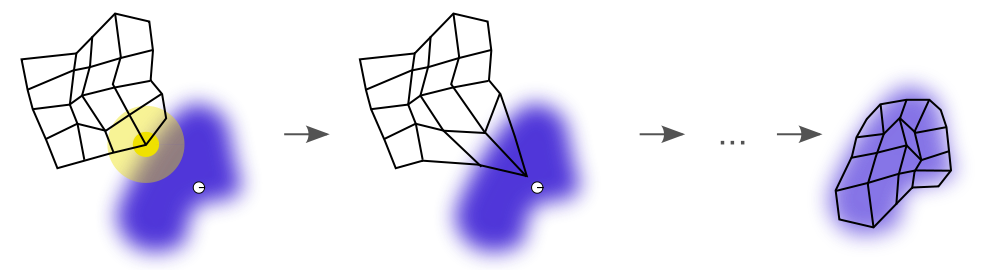
\includegraphics[scale=0.3]{som.png}
%        \centering
%        \caption{An illustration of the training of a self-organizing map. The blue blob is the distribution of the training data, and the small white disc is the current training datum drawn from that distribution. At first (left) the SOM nodes are arbitrarily positioned in the data space. The node (highlighted in yellow) which is nearest to the training datum is selected. It is moved towards the training datum, as (to a lesser extent) are its neighbors on the grid. After many iterations the grid tends to approximate the data distribution (right). \citep{wiki:som}}
%        \label{fig:som}
%\end{figure}

To organize the neurons, the SOM algorithm utilizes competitive learning, in which neurons compete among each other to represent input data vectors. Associated with each neuron is a weight vector with the same dimension as the input vectors. When the SOM considers a randomly-selected input vector, the neuron whose weight vector is ``closest'' to the input vector is deemed the winner. This nearest neuron is called the best matching unit (BMU). Then, the weights of the BMU and the neurons close to it in the SOM grid are adjusted towards the input vector. This procedure is repeated until convergence, at which point the neurons cease to ``move''---that is, their weight vectors do not change \citep{kohonen1990}. \par
%%%%%%%%%%%%%%%%%%%%%%%%%%%%%%%%%%%%%%%%%%%%%%%%%%%%%%%%%%%%%%%%%%%%%%%%%%%%%%%%%%%%
\begin{figure}[t]
        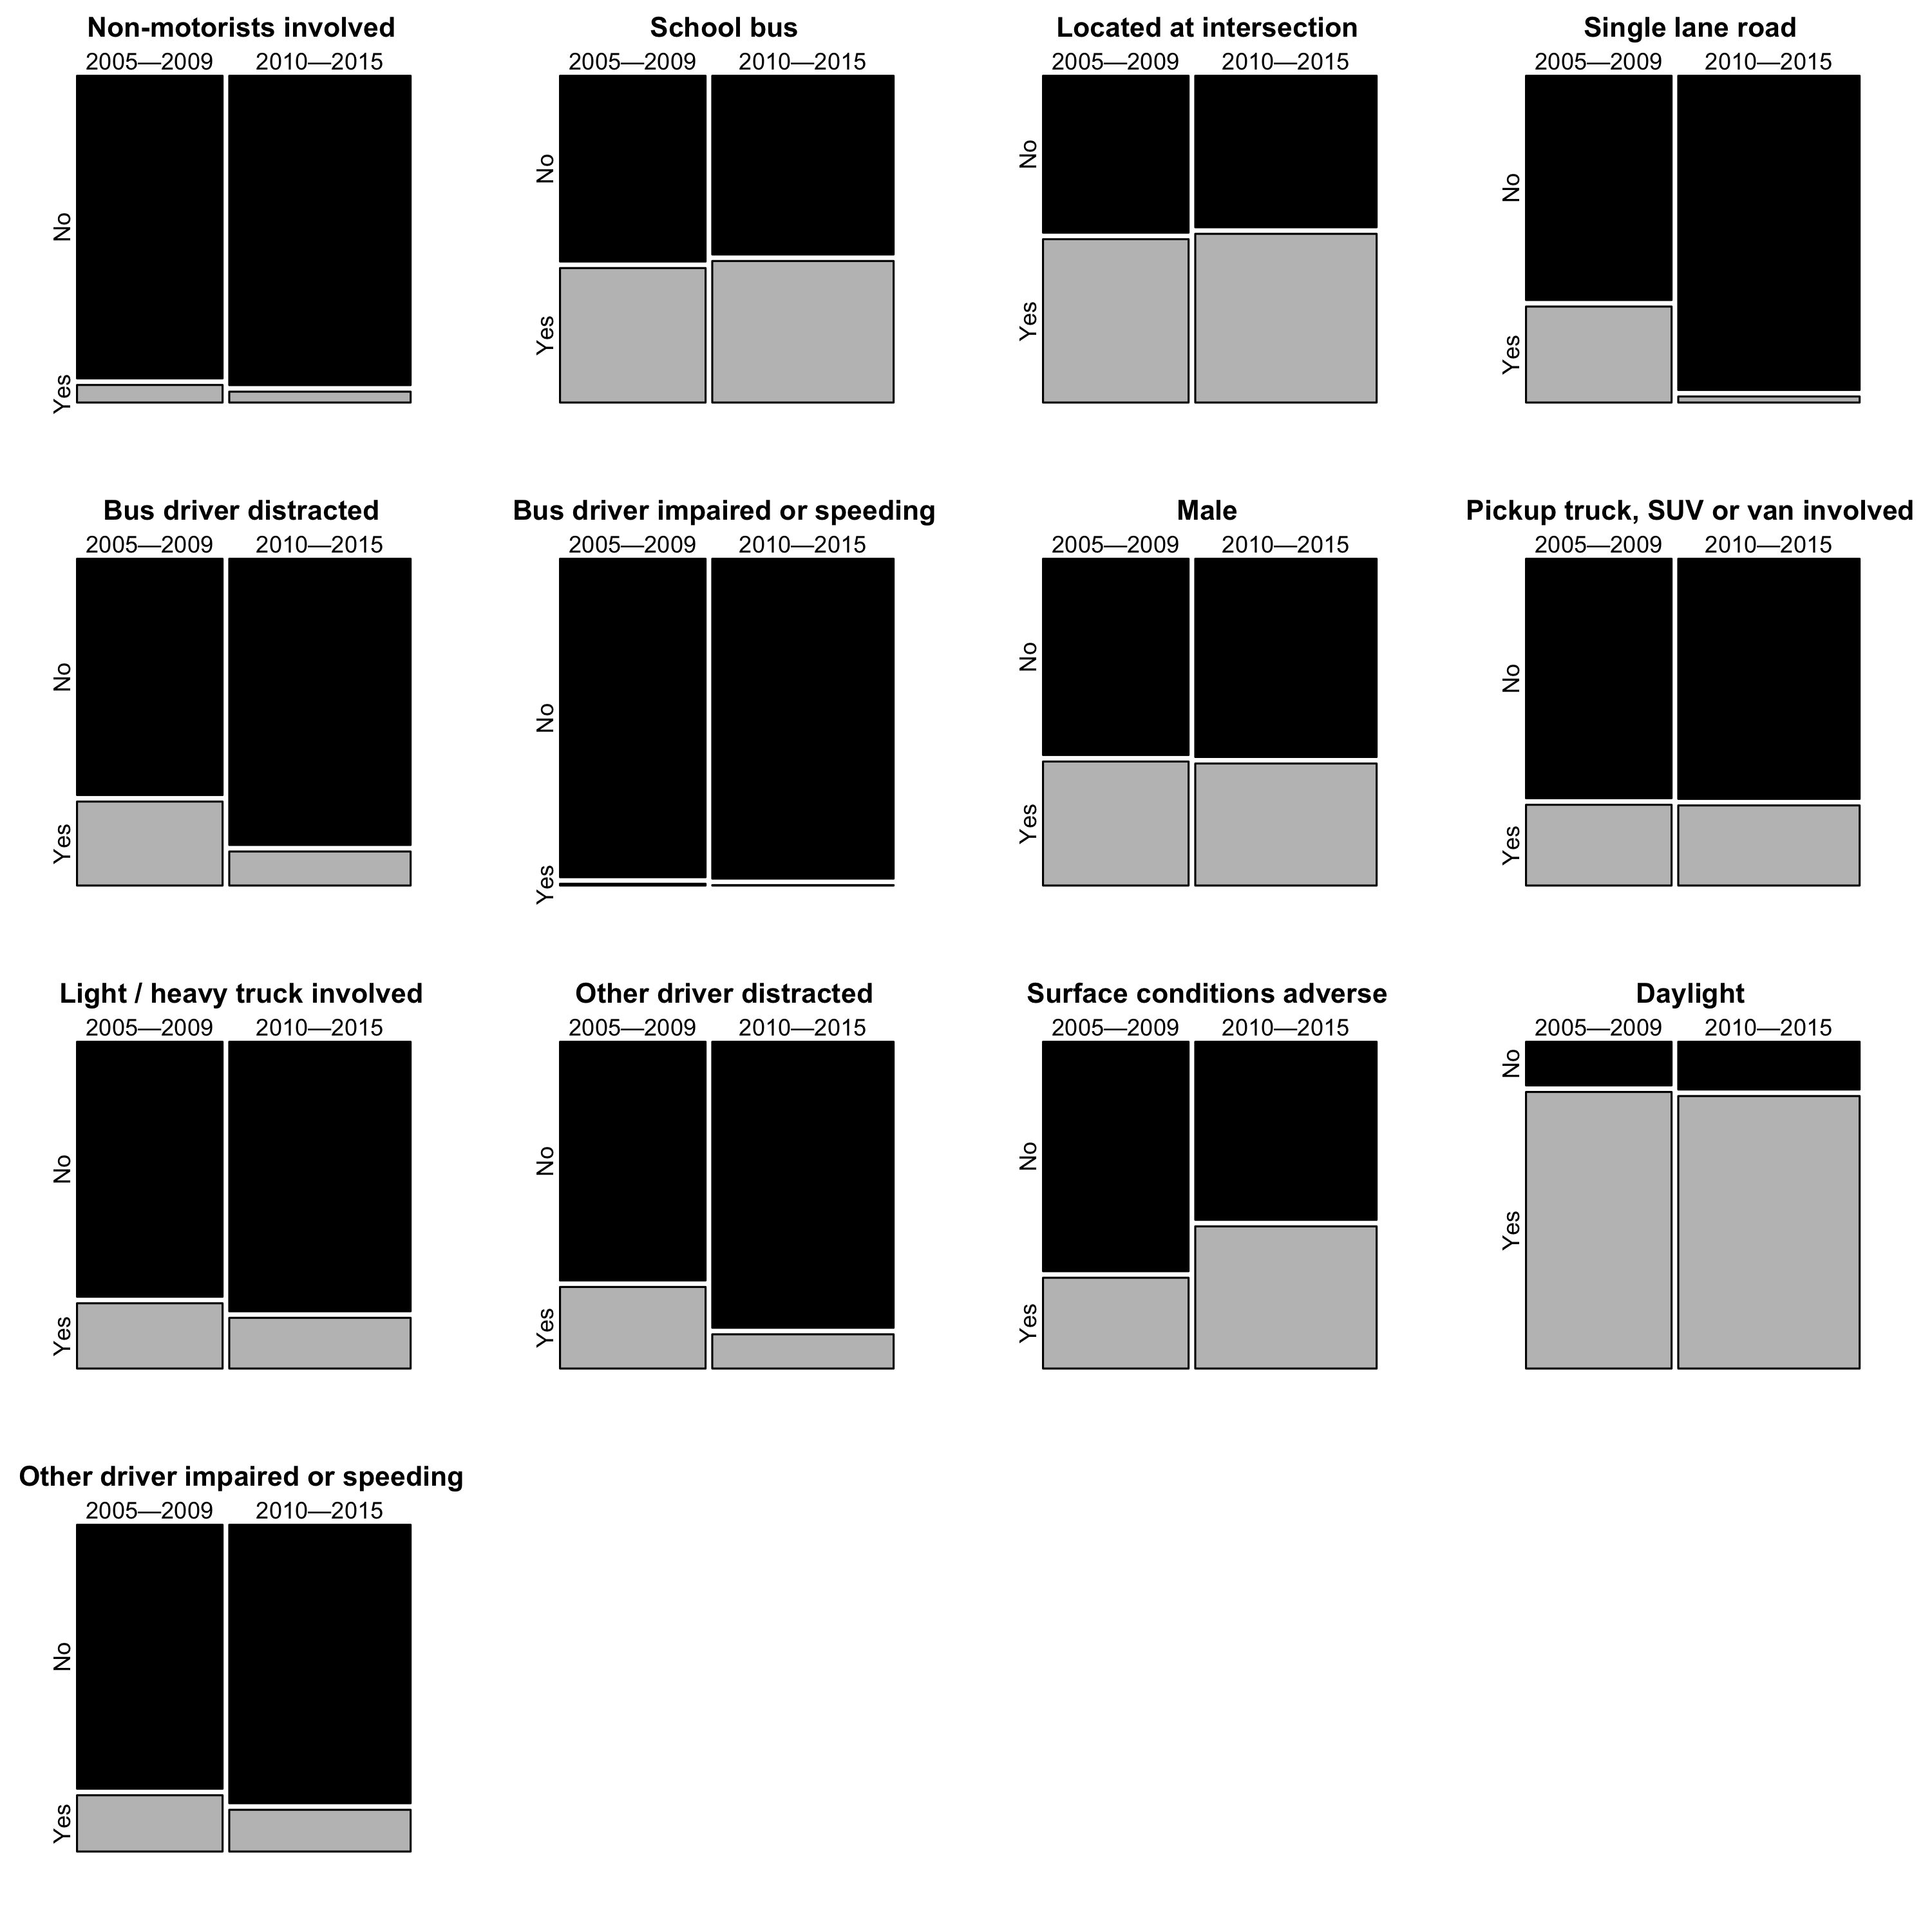
\includegraphics[width=\textwidth]{props.png}
                \caption{Mosaic plots comparing the binary response variables across the 2005--2009 
                and 2010--2015 datasets}
        \label{fig:props1}
\end{figure}
%%%%%%%%%%%%%%%%%%%%%%%%%%%%%%%%%%%%%%%%%%%%%%%%%%%%%%%%%%%%%%%%%%%%%%%%%%%%%%%%%%%%
In the second stage of clustering, we applied the neural gas algorithm of \citet{martinetz1991} to the self-organizing map from the first stage, thereby producing the final clustering.
The neural-gas clustering algorithm was historically inspired by the SOM algorithm and can be viewed a robust version of the sequential $K$-means algorithm \citep{macqueen1967}. In sequential $K$-means, cluster centers are updated by processing individual input vector sequentially. This contrasts with the approach of the traditional $K$-means algorithm, which considers all input vectors simultaneously. In the sequential method, only the cluster center closest to the input vector is adjusted towards it. The neural gas algorithm deviates from this by updating \emph{all} the cluster centers at each new input vector, with centers closer to the input vector adjusting more than those far away. This modification provides robustness to noisy input vectors and stabilizes the algorithm's convergence. \par

As mentioned previously, the SOM algorithm is a clustering algorithm in its own right, and hence could be used to form the taxonomy of bus crashes by itself. However, as mentioned in \citet{prato2013bus}, the neural-gas algorithm has advantages over methods like SOM in terms of convergence speed and accuracy \citep{vesanto2000}. The high computational complexity of the neural-gas algorithm, its main disadvantage, is mitigated by its application to the lower-dimensional SOM neuron grid. This allows more flexibility in dealing with high-dimensional output, without sacrificing the practicality of applying the technique. \par
%%%%%%%%%%%%%%%%%%%%%%%%%%%%%%%%%%%%%%%%%%%%%%%%%%%%%%%%%%%%%%%%%%%%%%%%%%%%%%%%%%%%
\begin{figure}[t]
        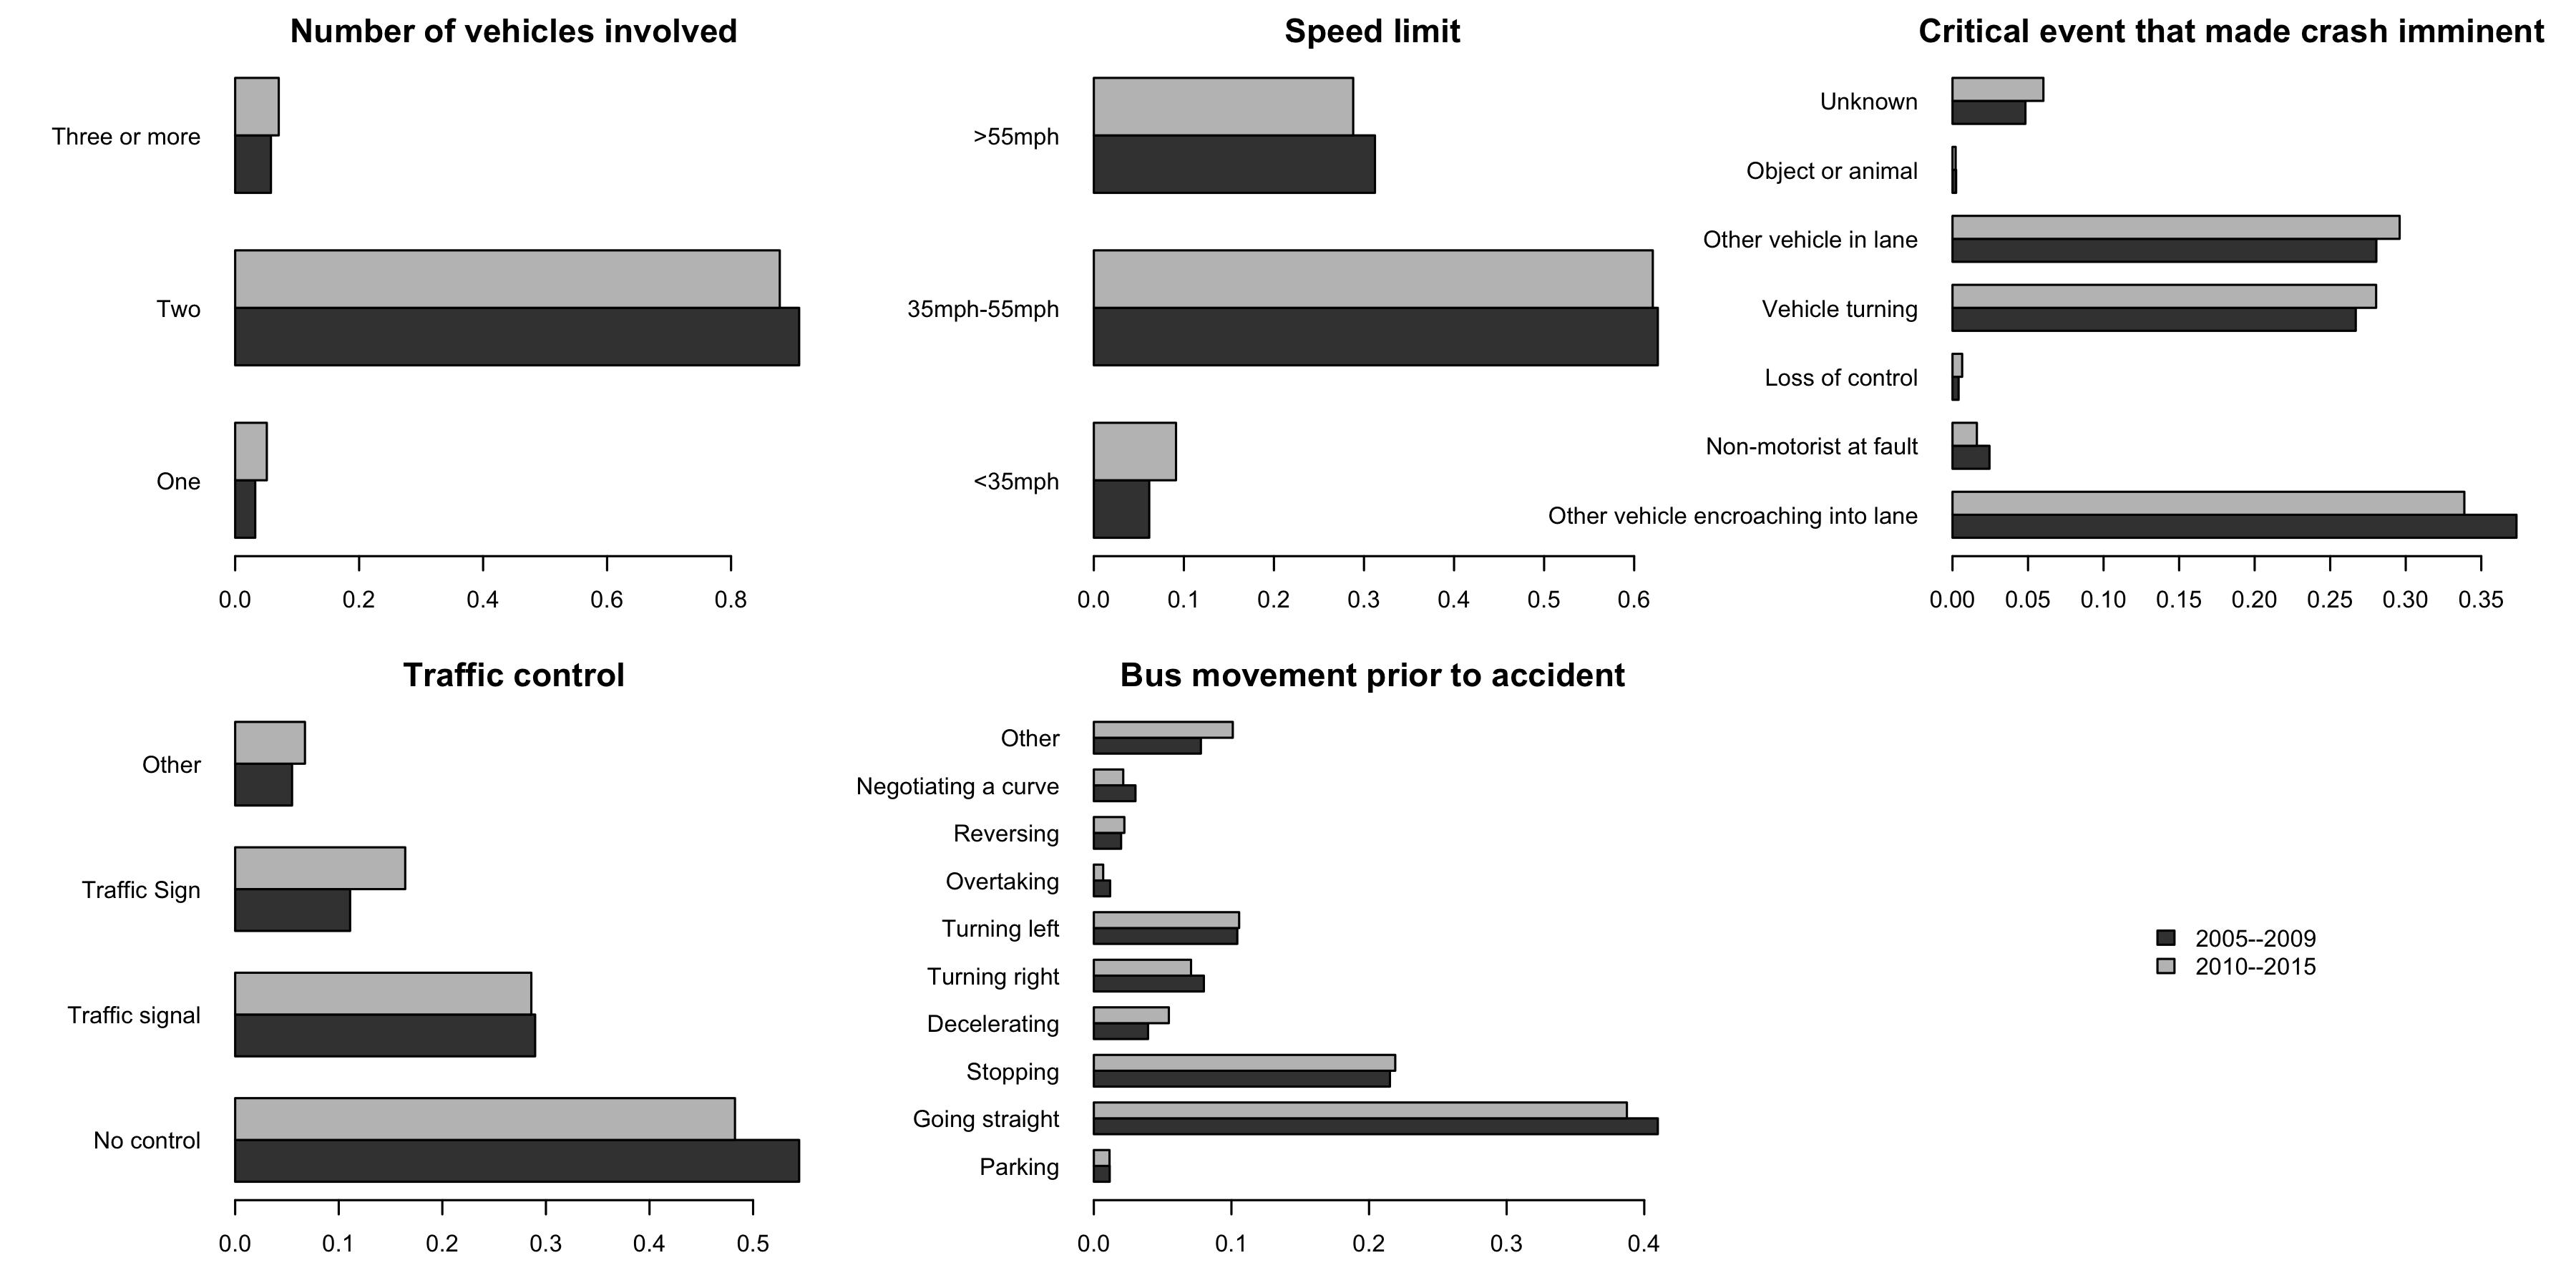
\includegraphics[width=\textwidth]{radar-bar.png}
                \caption{Grouped bar plots comparing the categorical response variables across the 2005--2009 and 2010--2015 datasets.}
        \label{fig:cat1}
\end{figure}
%%%%%%%%%%%%%%%%%%%%%%%%%%%%%%%%%%%%%%%%%%%%%%%%%%%%%%%%%%%%%%%%%%%%%%%%%%%%%%%%%%%%


\section{Results} \label{sec:results}
A total of 4386 bus accidents were reported in the GES data from 2005--2015, representative of an approximate total of 530797 bus accidents. We performed basic exploratory data analysis to identify relevant clustering variables, and to compare the data composition across the two time periods.

Figure \ref{fig:props1} compares the proportion of ``yes'' responses for the binary variables. Generally, the proportions are consistent across the two time periods. We see a decrease in driver distraction in the later dataset, and a proportional increase in the accidents in the presence of adverse surface conditions. Other-driver distraction fell by almost 50\% in the later dataset. Incidents where the other driver was impaired or under the influence of alcohol or drugs also fell in the later years by a comparatively small proportion. We also observe that in both time periods very few incidents involved bus drivers driving while impaired. But, these variables reflect only a small portion of the explanatory variables, so that for the most part, the two datasets are similar in terms of their binary responses.
%%%%%%%%%%%%%%%%%%%%%%%%%%%%%%%%%%%%%%%%%%%%%%%%%%%%%%%%%%%%%%%%%%%%%%%%%%%%%%%%%%%%%
%\begin{figure}[t]
%        \caption{Mosaic plots comparing the binary response variables across the 2005--2009 
%                and 2010--2015 datasets}
%        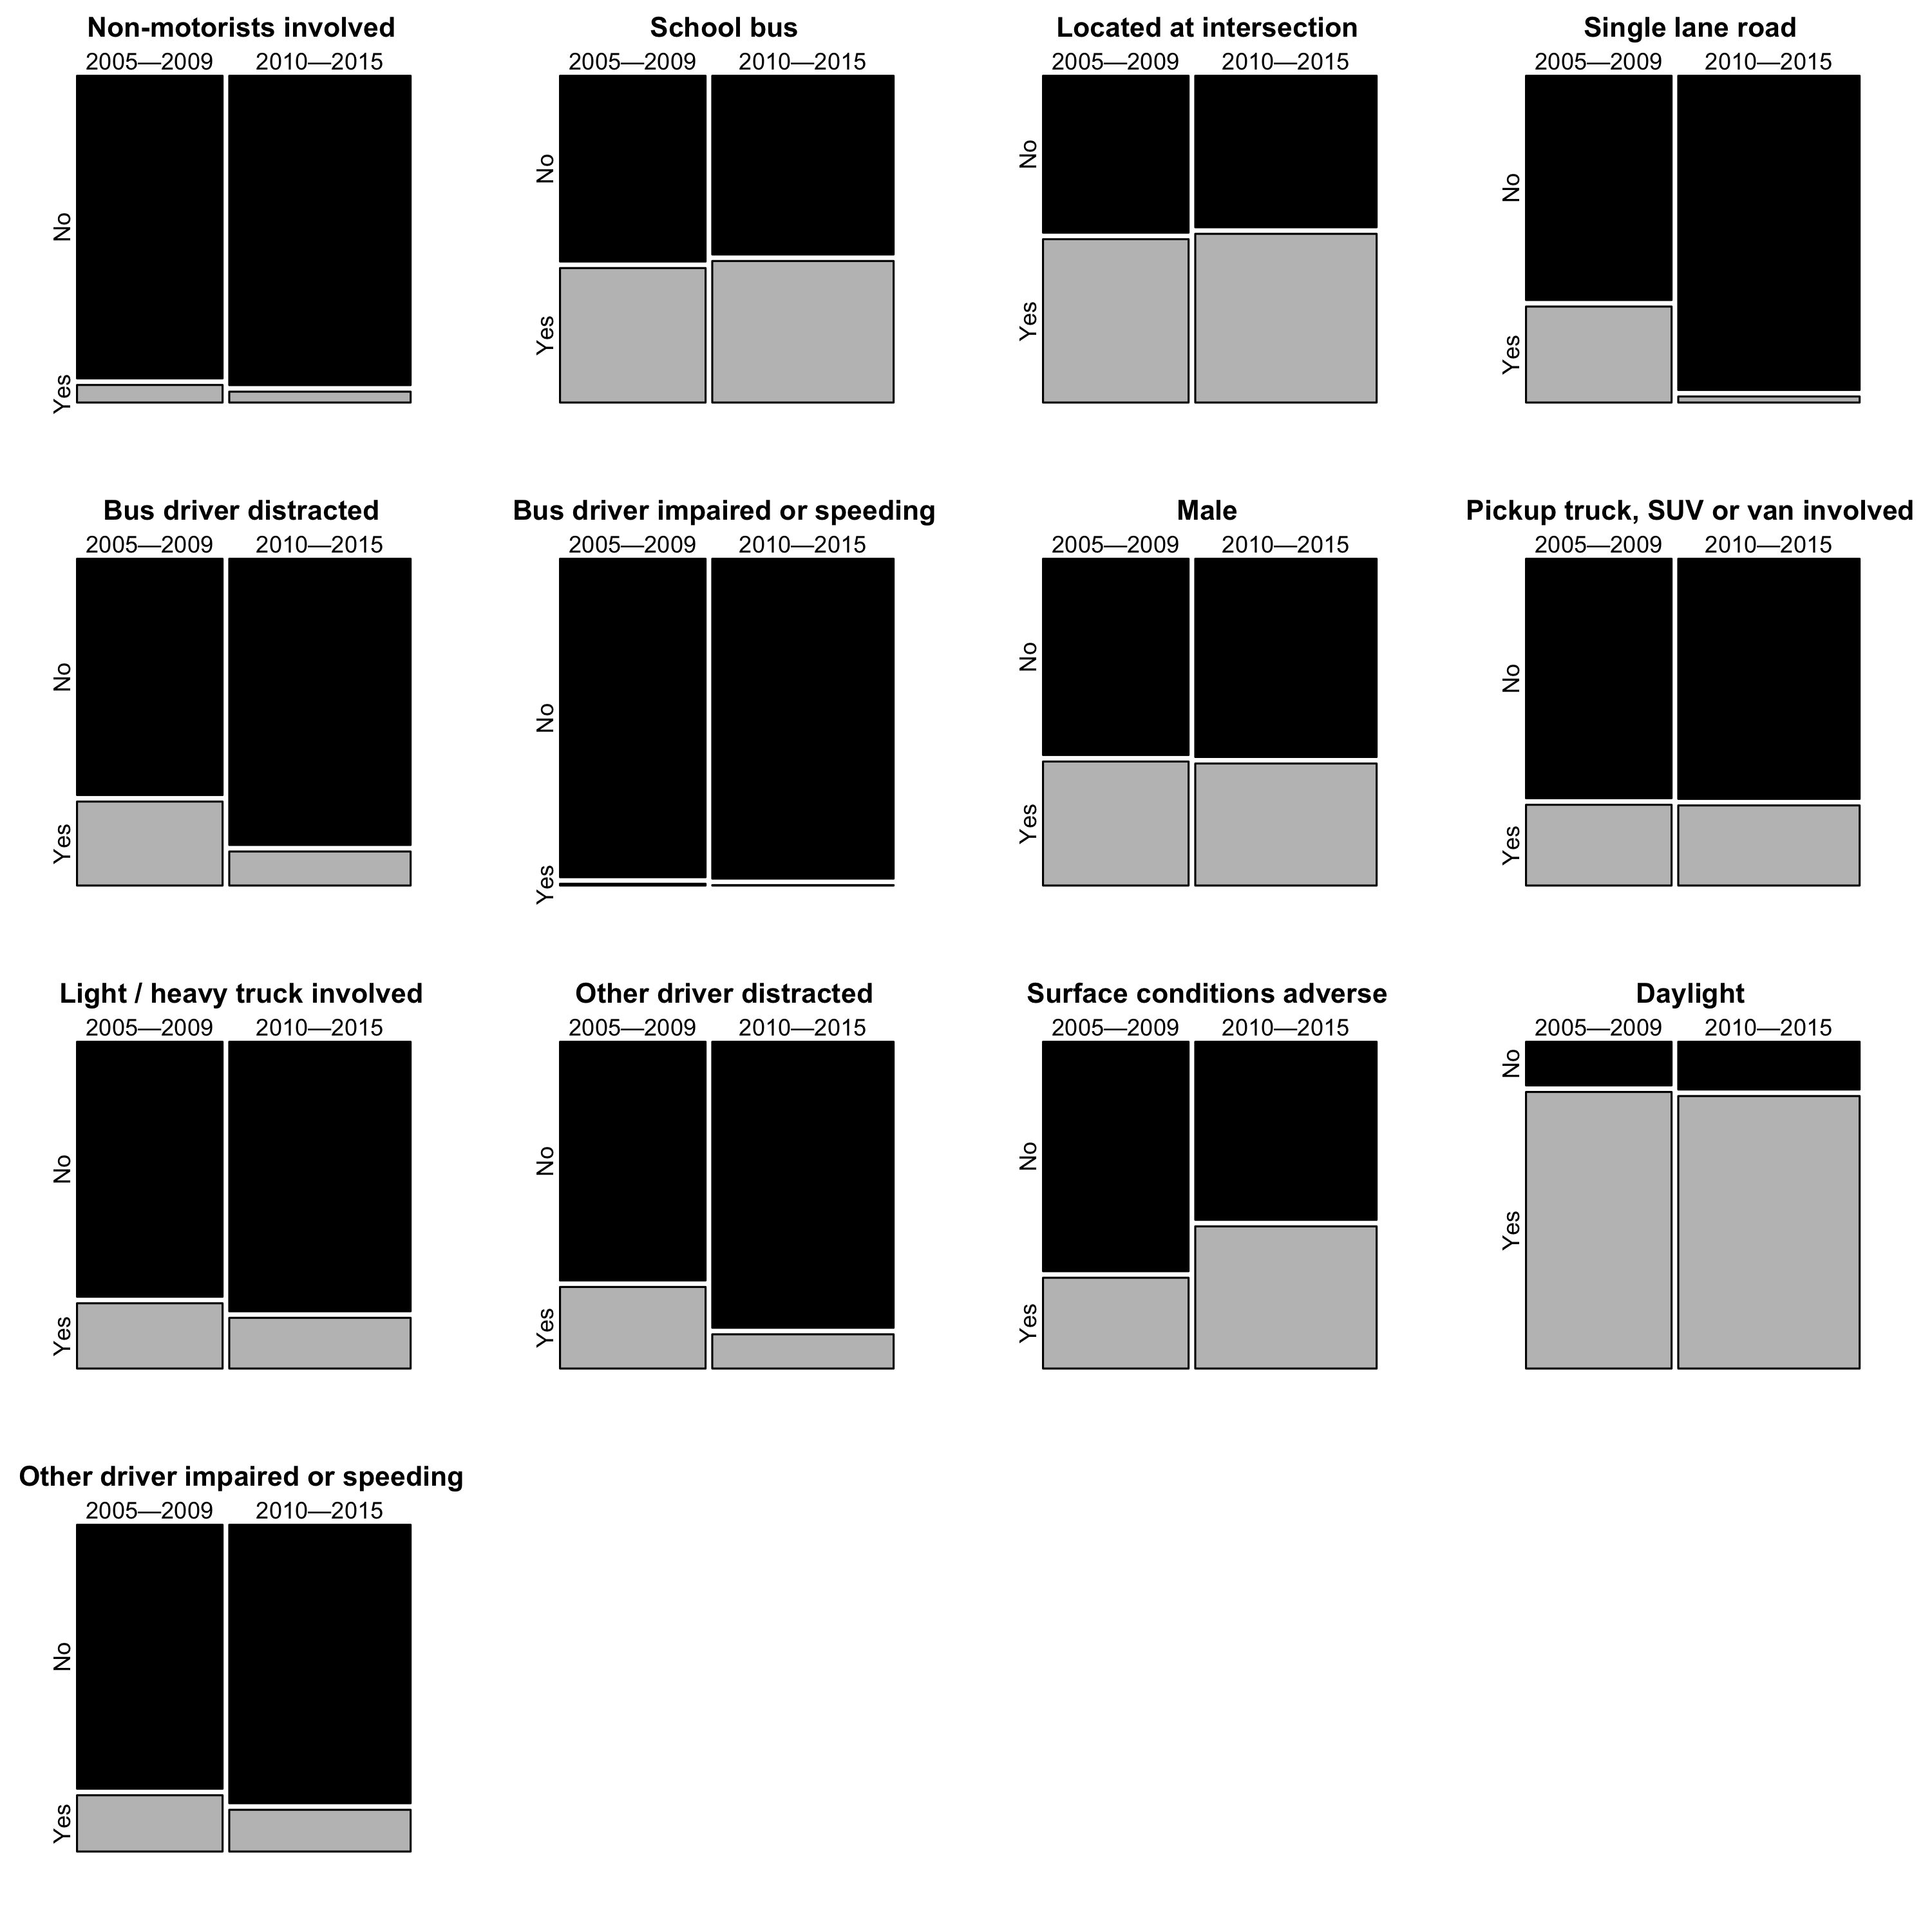
\includegraphics[width=\textwidth]{props.png}
%        \label{fig:props1}
%\end{figure}
%%%%%%%%%%%%%%%%%%%%%%%%%%%%%%%%%%%%%%%%%%%%%%%%%%%%%%%%%%%%%%%%%%%%%%%%%%%%%%%%%%%%%
%
%Figure \ref{fig:cat1} gives grouped bar plots for the categorical variables considered in the analysis. As these plots indicate, there are noticeable differences in the distribution of the variables for traffic control, critical event that made the crash imminent, and bus movement prior to the event. These variables seem to be distributed differently in the two time periods, information which is used in the clustering.
%%%%%%%%%%%%%%%%%%%%%%%%%%%%%%%%%%%%%%%%%%%%%%%%%%%%%%%%%%%%%%%%%%%%%%%%%%%%%%%%%%%%%
%\begin{figure}[t]
%        \caption{Grouped bar plots comparing the categorical response variables across the 2005--2009 and 2010--2015 datasets.}
%        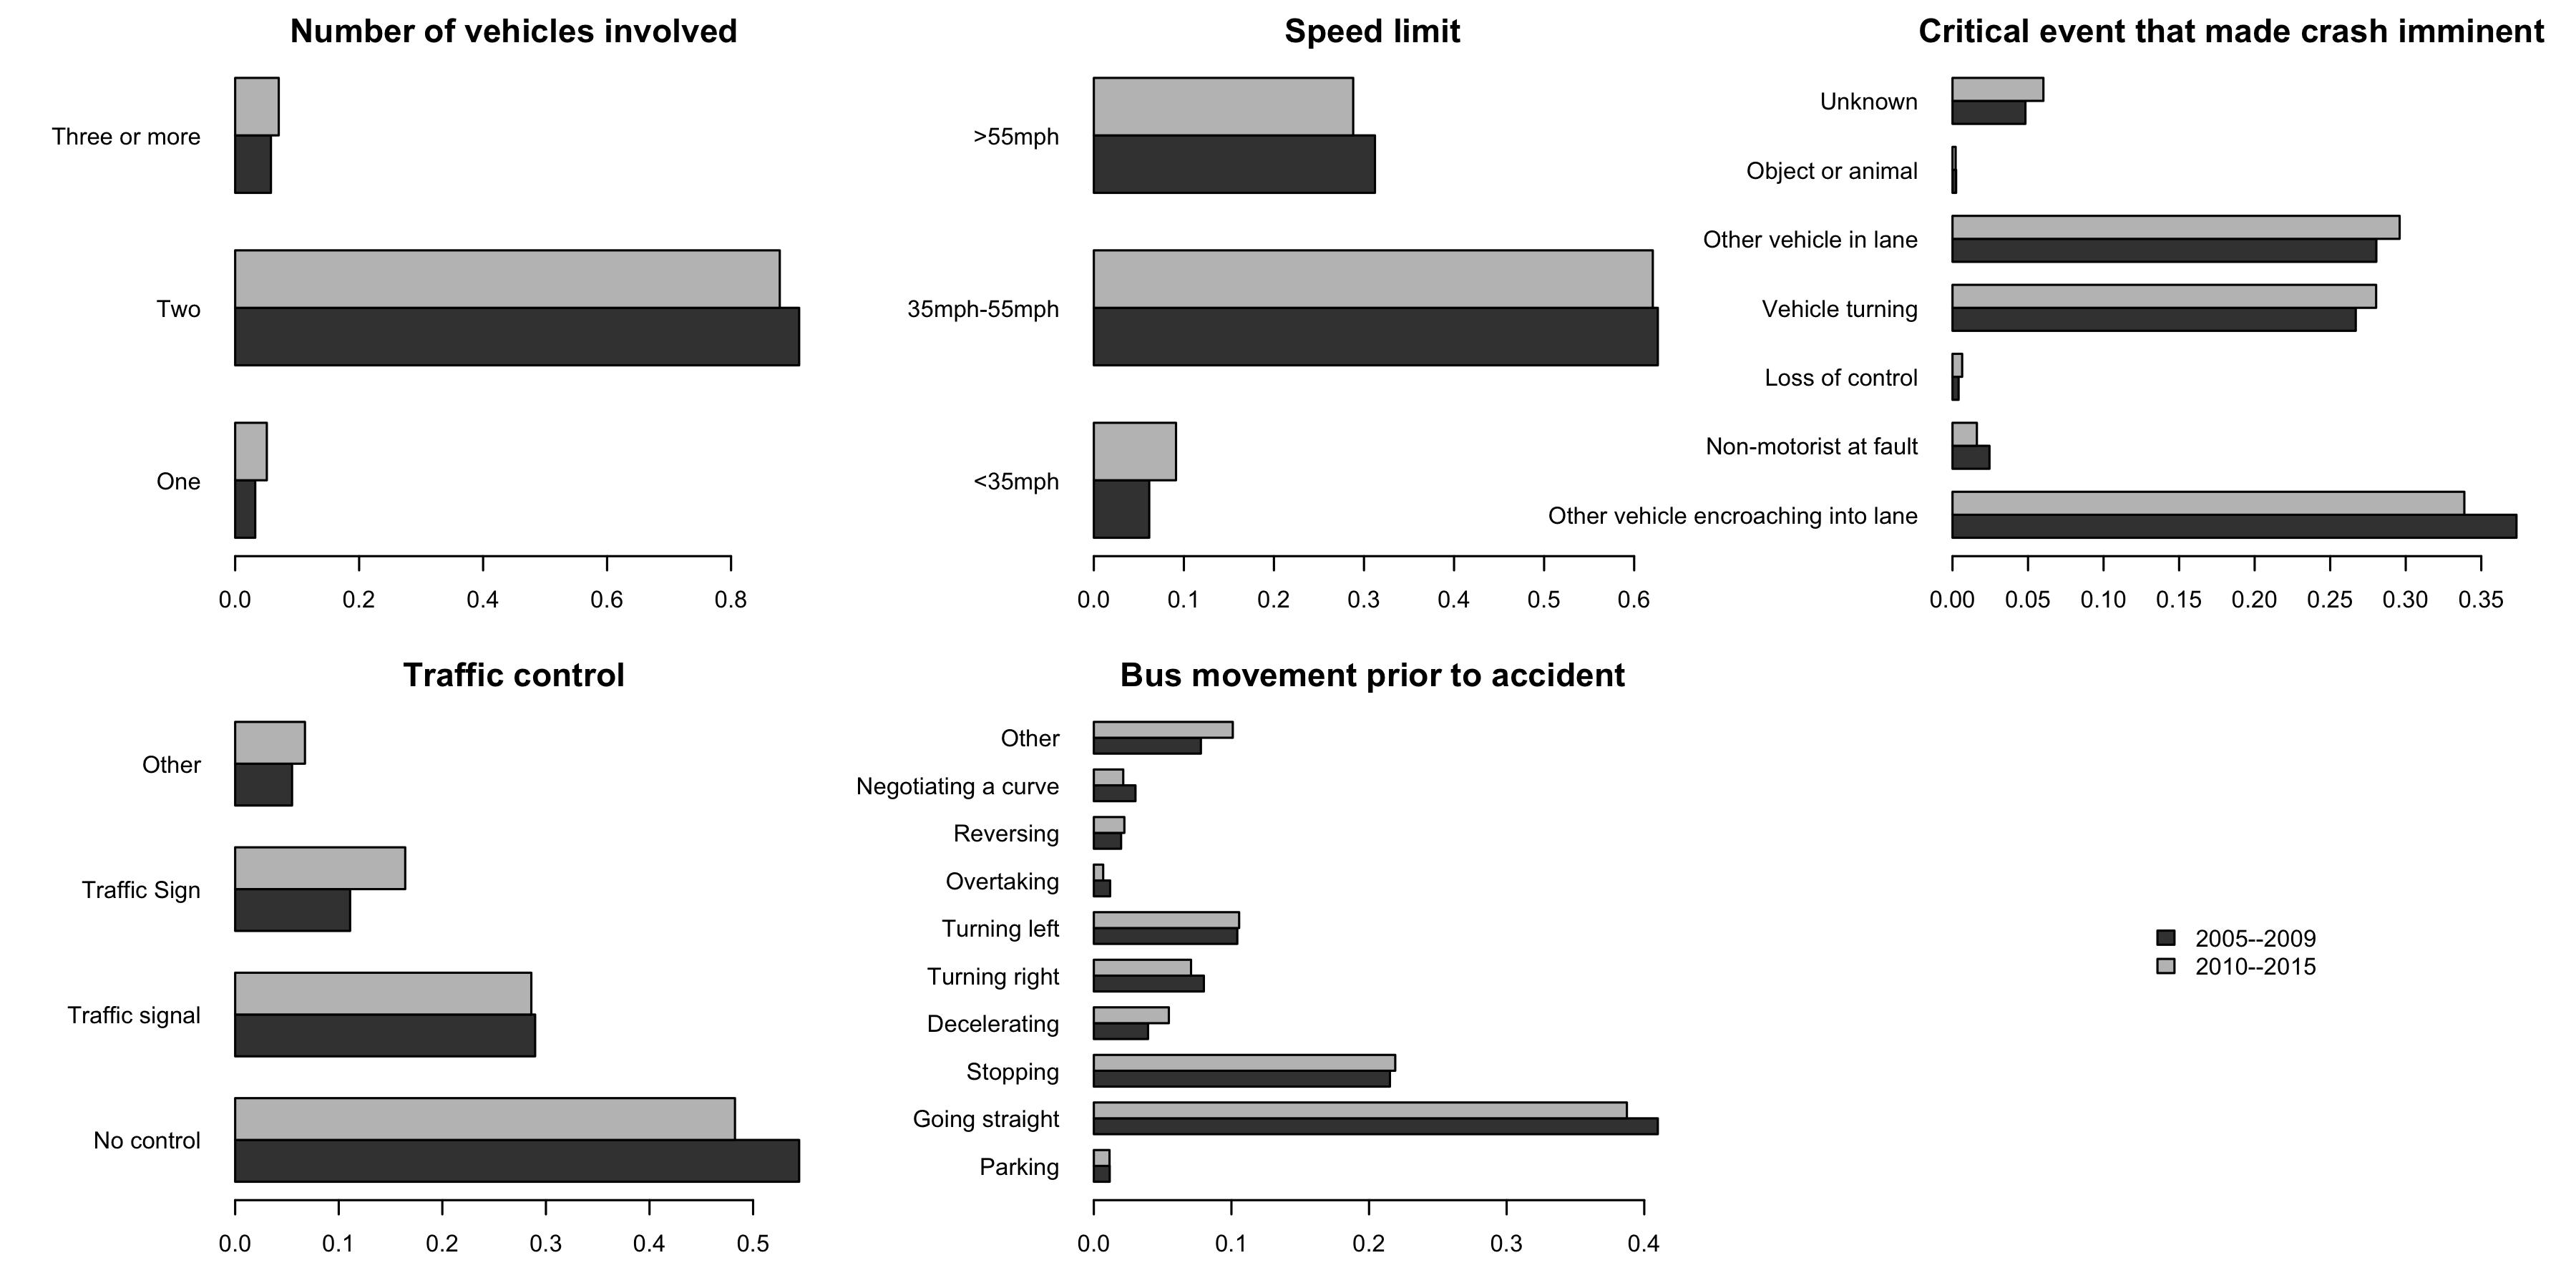
\includegraphics[width=\textwidth]{radar-bar.png}
%        \label{fig:cat1}
%\end{figure}
%%%%%%%%%%%%%%%%%%%%%%%%%%%%%%%%%%%%%%%%%%%%%%%%%%%%%%%%%%%%%%%%%%%%%%%%%%%%%%%%%%%%%

We chose a $20\times 20$ grid of neurons for the SOM clustering method, similar to \citet{prato2013bus}. The neural gas algorithm partitioned the data into four clusters, which we chose to optimally balance cluster homogeneity and differentiation. We used the R programming language \citep{r:r} to implement the two-stage clustering. We performed SOM using the package ``kohonen'' \citep{r:kohonen}, \citep{r:r} and we used ``cclust'' for the neural gas algorithm \citep{r:cclust}, \citep{r:r}.

Based on the results of the analysis, the four clusters in the \textbf{2005--2009 dataset} can be described as follows:

%%%%%%%%%%%%%%%%%%%%%%%%%%%%%%%%%%%%%%%%%%%%%%%%%%%%%%%%%%%%%%%%%%%%%%%%%%%%%%%%%%%%
\begin{figure}[t]
        %\centering
        \begin{subfigure}[t]{.5\textwidth}
%  \centering
                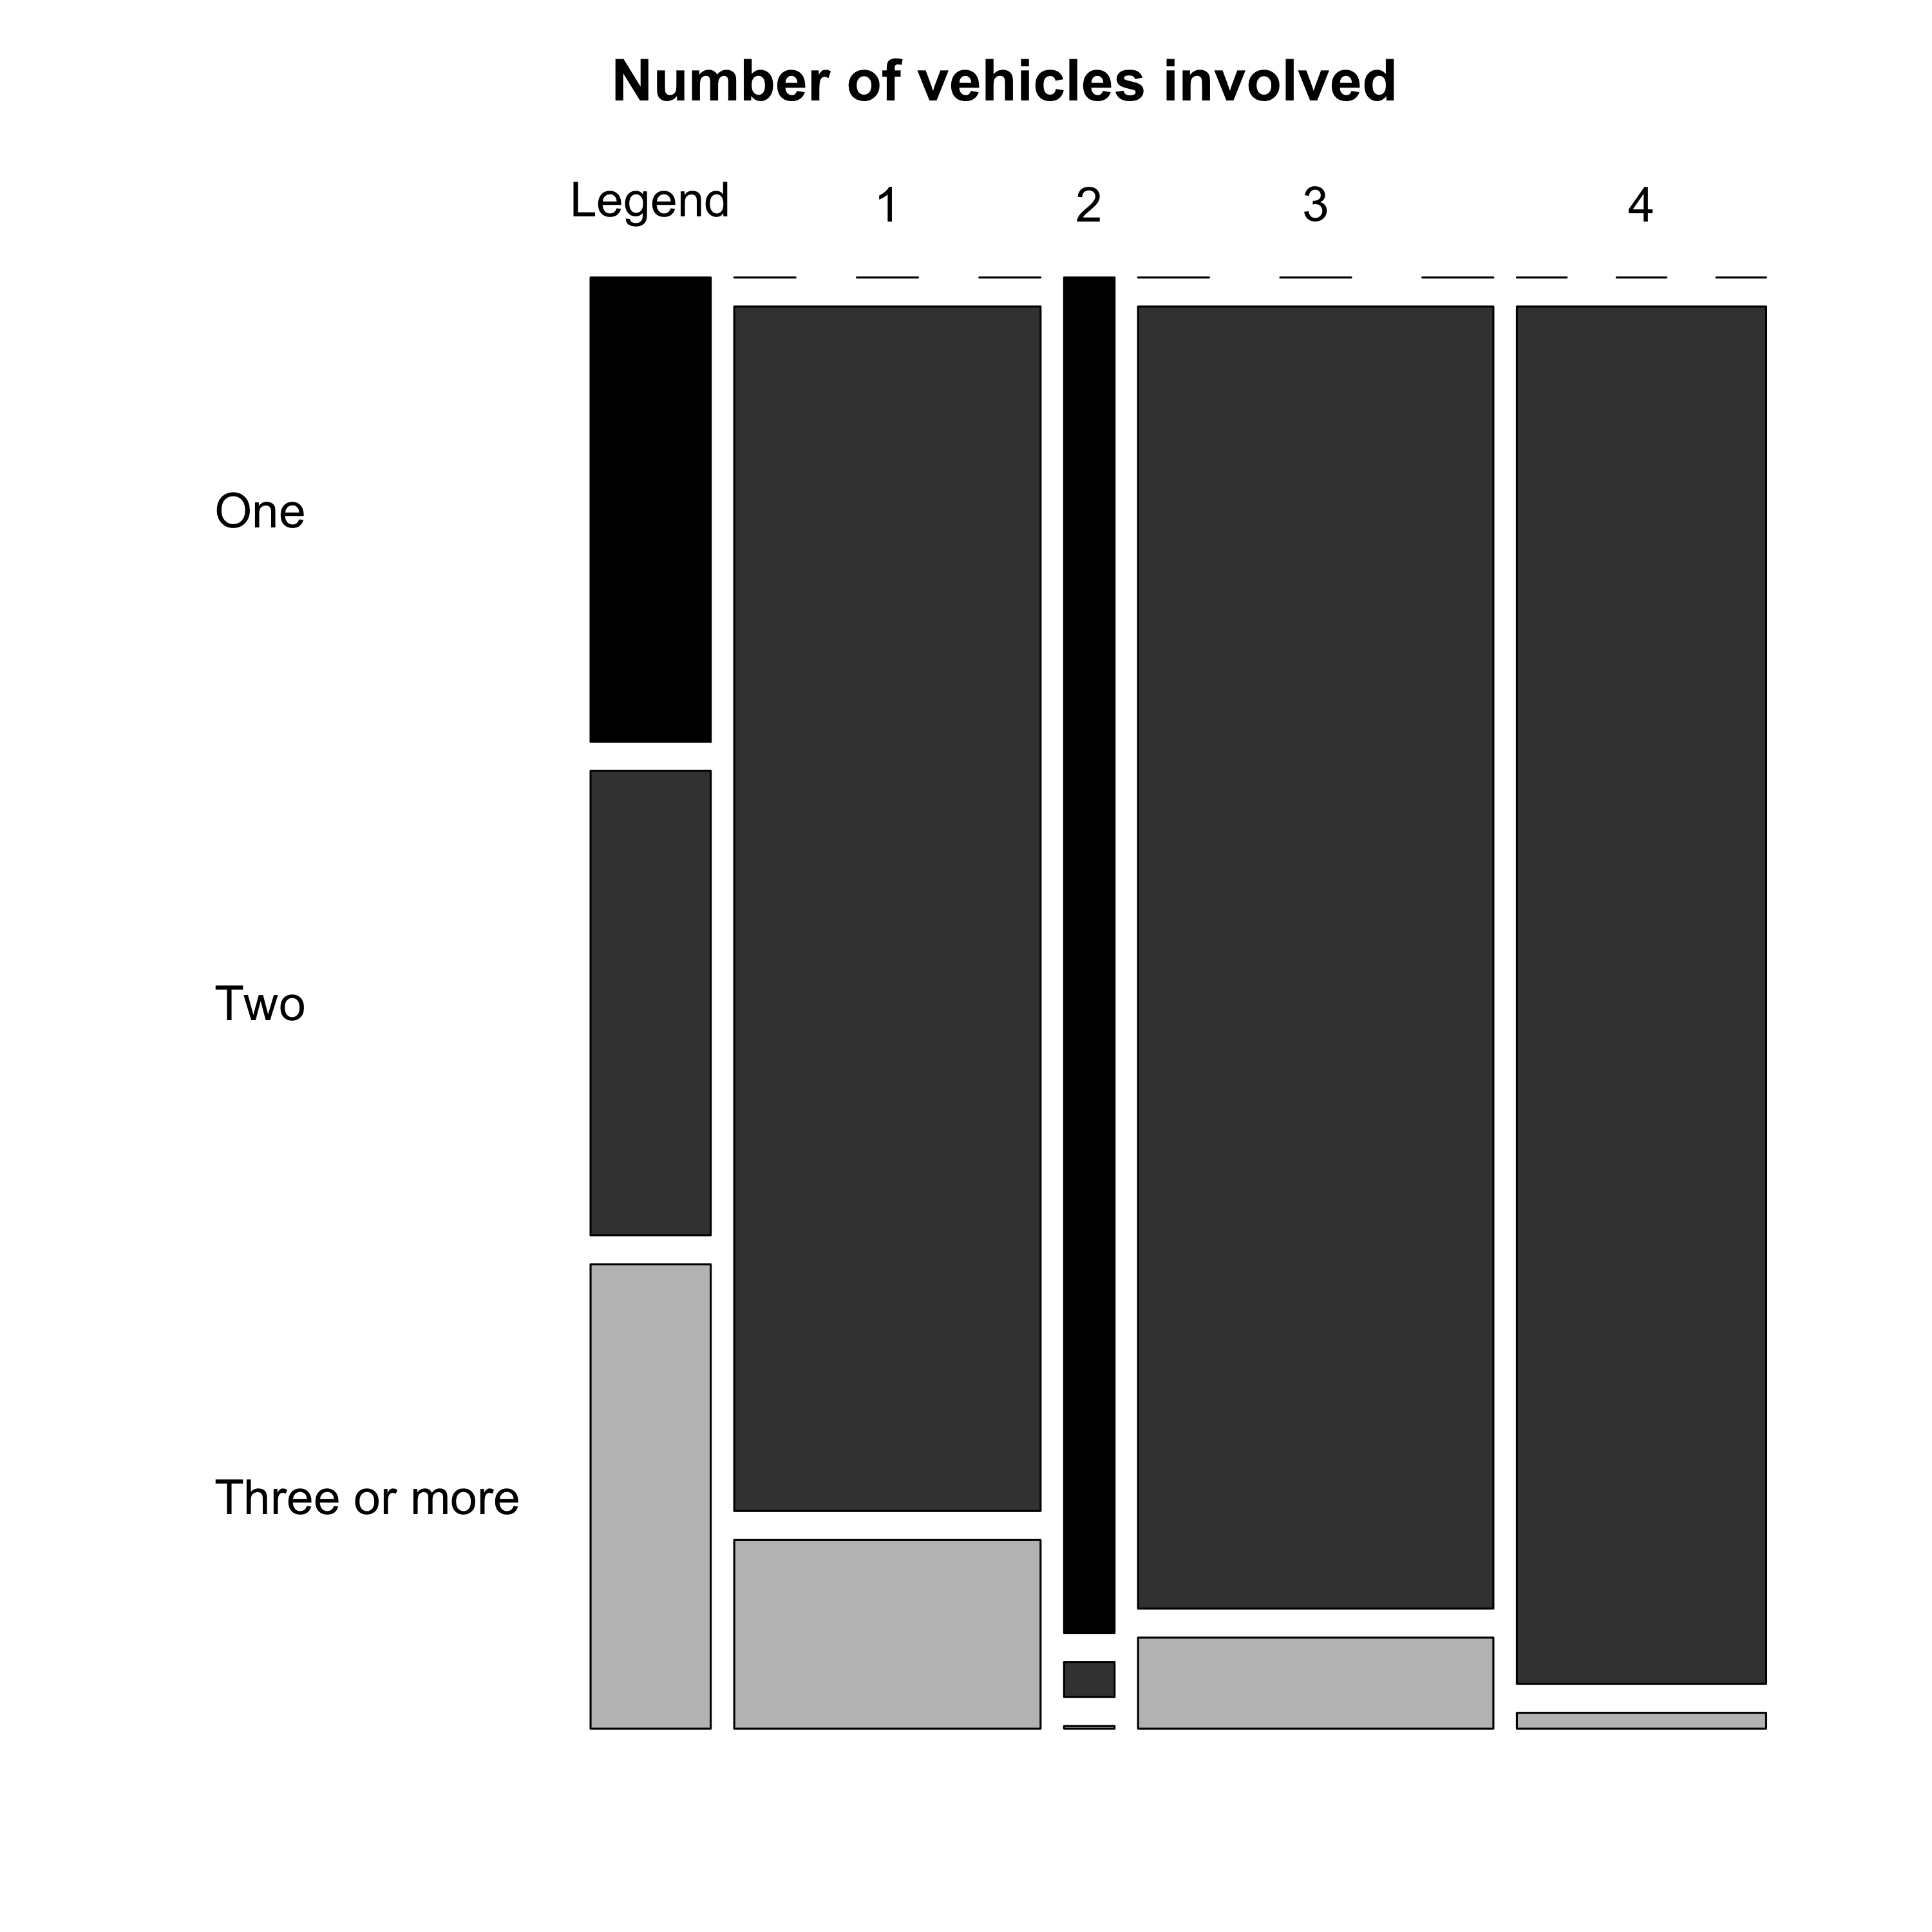
\includegraphics[width=1\linewidth]{veh_invl_0509.png}
                \caption{2005--2009}
        \end{subfigure}%
        \begin{subfigure}[t]{.5\textwidth}
%  \centering
                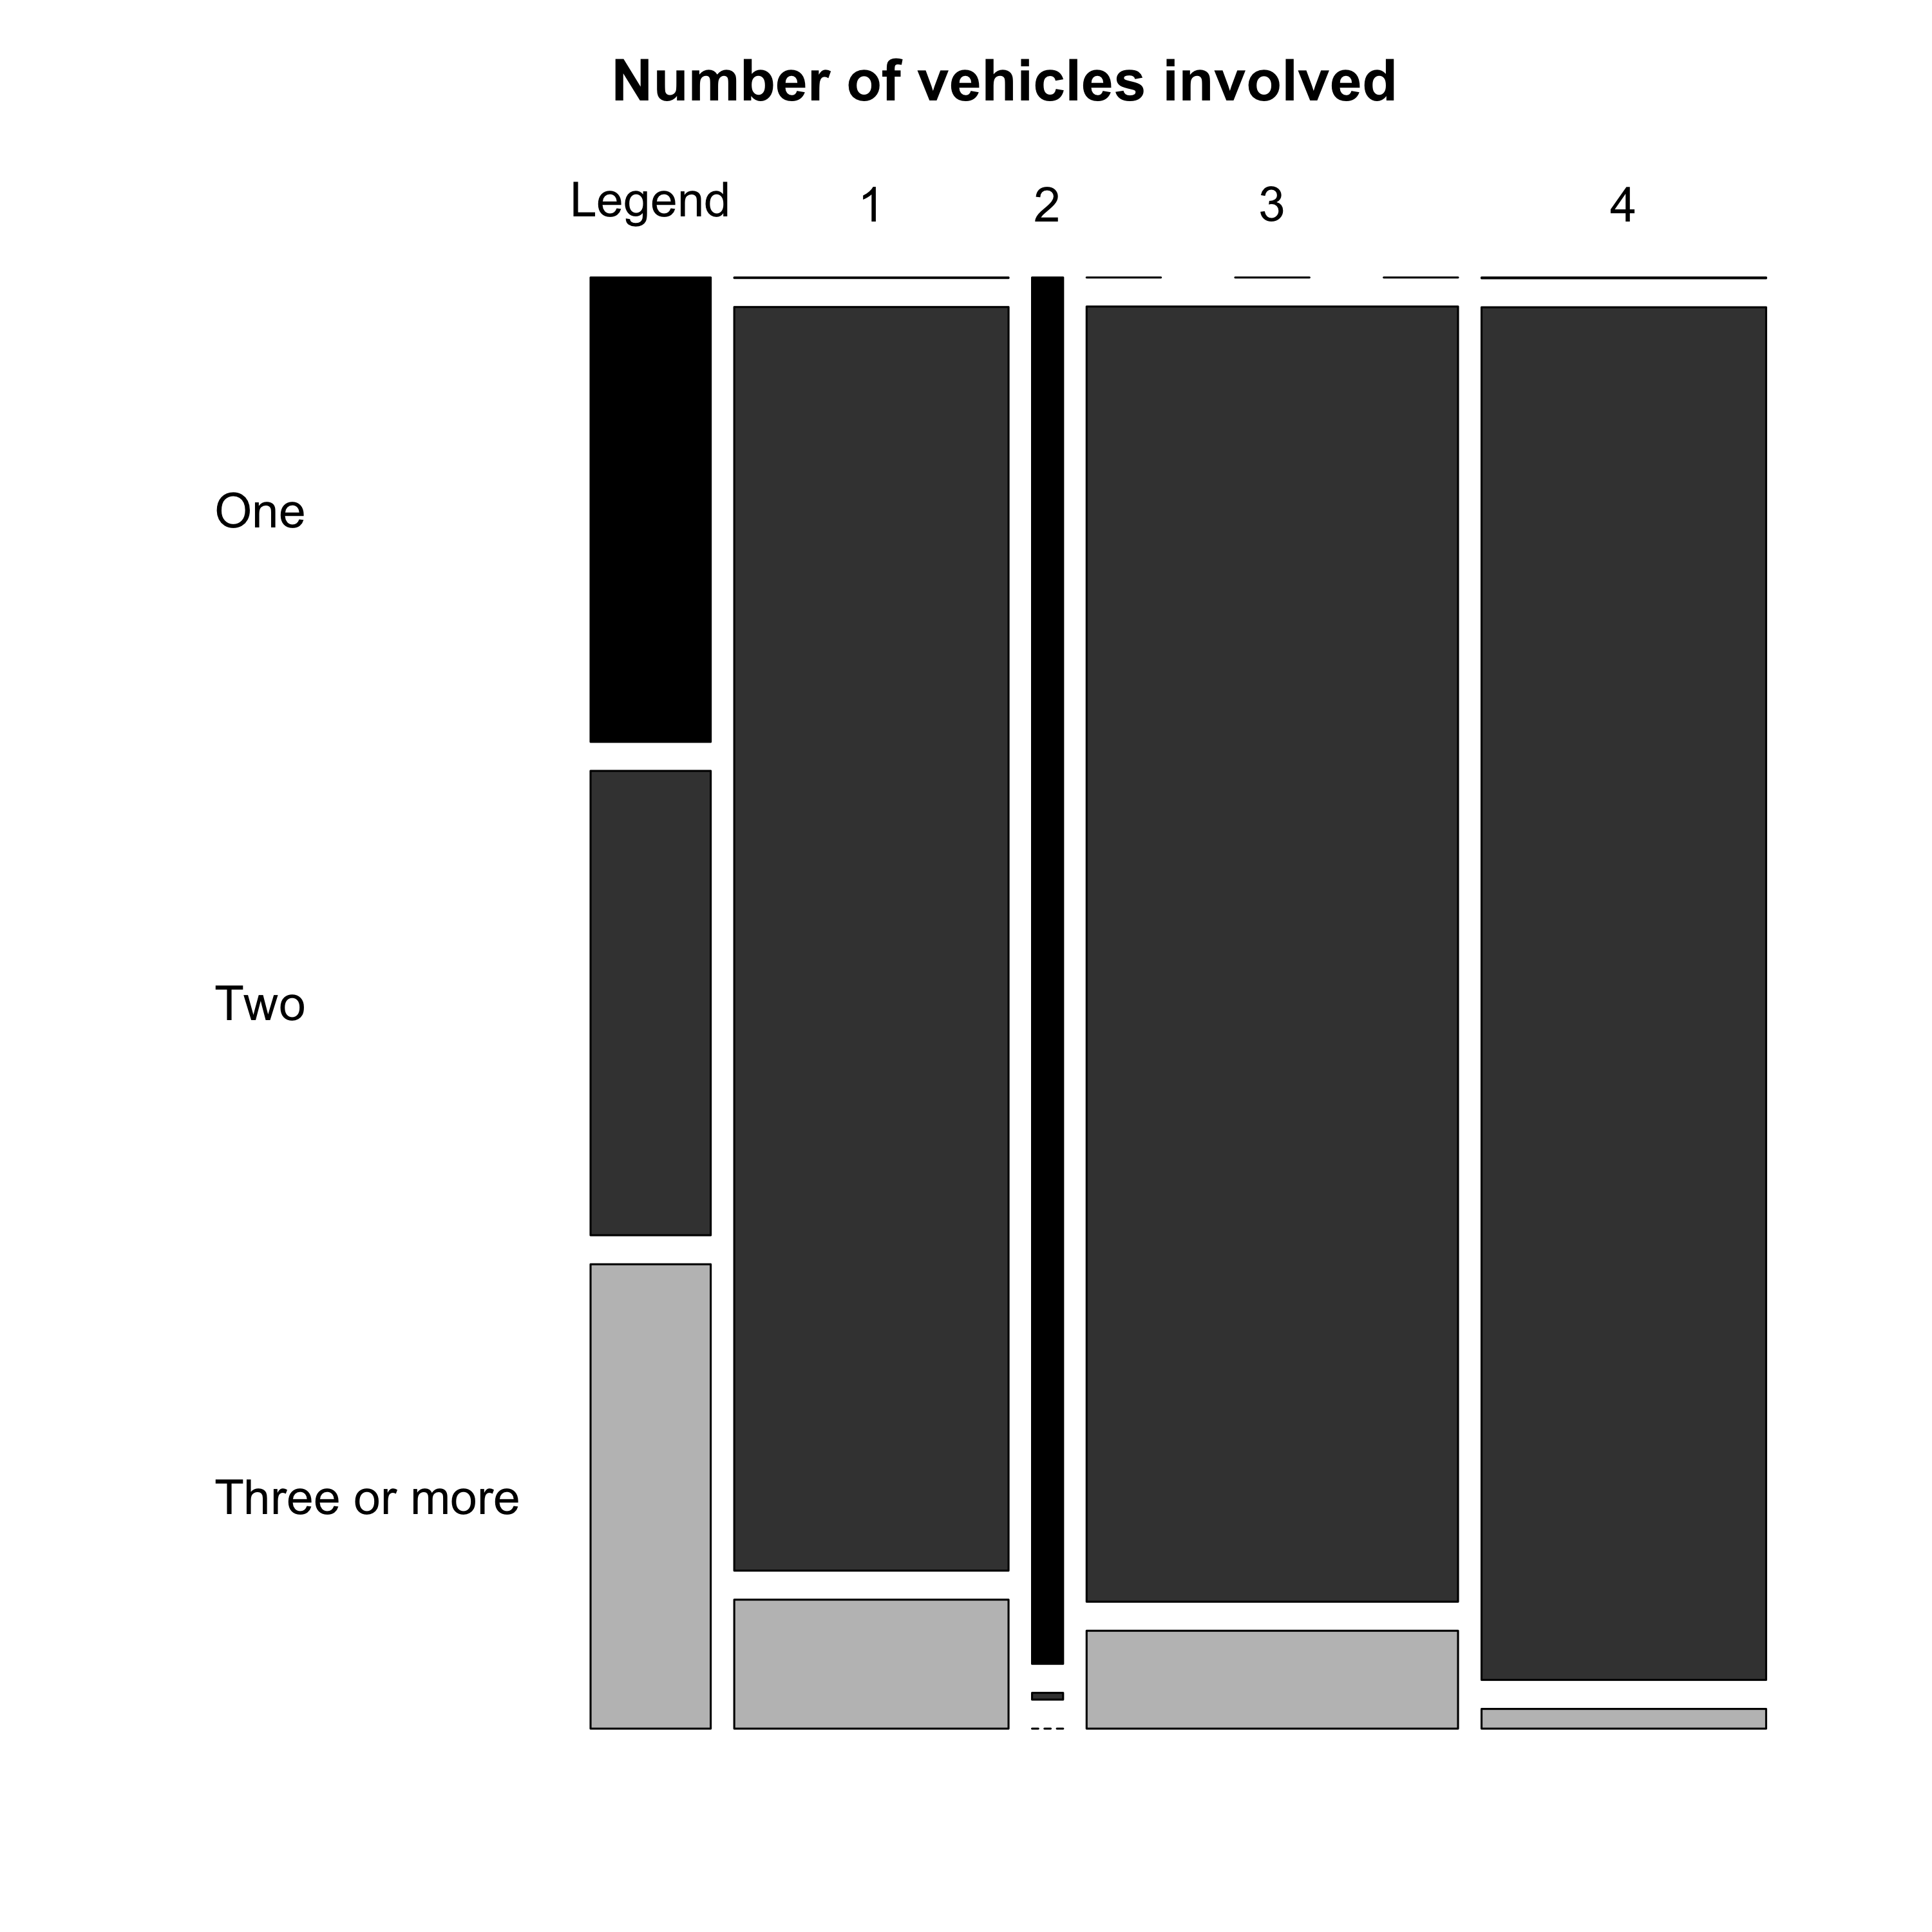
\includegraphics[width=1\linewidth]{veh_invl.png}
                \caption{2010--2015}
        \end{subfigure}
        \caption{Mosaic plots giving the breakdown of the variable ``number of vehicles involved in the accident'' for each of the four clusters.}
 \label{fig:clus10}
\end{figure}
%%%%%%%%%%%%%%%%%%%%%%%%%%%%%%%%%%%%%%%%%%%%%%%%%%%%%%%%%%%%%%%%%%%%%%%%%%%%%%%%%%%%

\noindent
\textbf{Cluster 1}: Single vehicle crashes involving non-motorists (100\%), (Figure \ref{fig:clus10} (a)) that happened when the bus was going straight (37.8\%), turning left (19.4\%) or trying to park (15.1\%) (Figure \ref{fig:clus4} (a)). There were two primary reasons for the crash: the bus turned (49.2\%), or the non-motorist (pedestrians, cyclists, bicyclists, etc.) was at fault (29\%) (Figure \ref{fig:clus12} (a)). In 35.8\% of the cases, the bus driver admitted to have been distracted. 40.8\% of the time, a school bus was involved. 4.7\% of the cases involved the non-motorist being impaired or under the influence. 42.9\% of the crashes happened at an intersection. 71.3\% of the crashes happened where the road had no traffic control, and in 14.3\% of the cases there was a traffic signal (Figure \ref{fig:clus8} (a)). 

\noindent
\textbf{Cluster 2}: Multi-vehicle crashes (93.1\% involving two vehicles) that occurred when the bus was going straight (64.2\%) or stopping (17.3\%). The crash was primarily due to the other vehicle encroaching into the bus' lane (92.1\%), implying that the crash was mainly the other driver's fault. In 19.7\% of the cases, the bus driver admitted to have been distracted, and 39.1\% of the time, a school bus was involved. Most of the crashes happened on roadways with moderate to high speed limits (61.5\% on roads with 35--55 MPH and 29.3\% on roads with greater than 55 MPH, Figure \ref{fig:clus6} (a)). For 25.6\% of the crashes, at least one of the other drivers involved was distracted, and 21.0\% of the cases involved at least one of the other drivers being impaired or under the influence. 50.3\% of the crashes happened at an intersection. 49.9\% of the crashes happened where the road had no traffic control, for 27.2\% of the cases there was a traffic signal, and in 18.1\% of the cases there was a traffic sign. 23.4\% of the cases involved a light or a heavy truck, and 23.1\% of the crashes involved an SUV, pickup truck, or van (Figure \ref{fig:clus2} (a)).

%%%%%%%%%%%%%%%%%%%%%%%%%%%%%%%%%%%%%%%%%%%%%%%%%%%%%%%%%%%%%%%%%%%%%%%%%%%%%%%%%%%%
\begin{figure}[t]
%\centering
        \begin{subfigure}{.5\textwidth}
%  \centering
                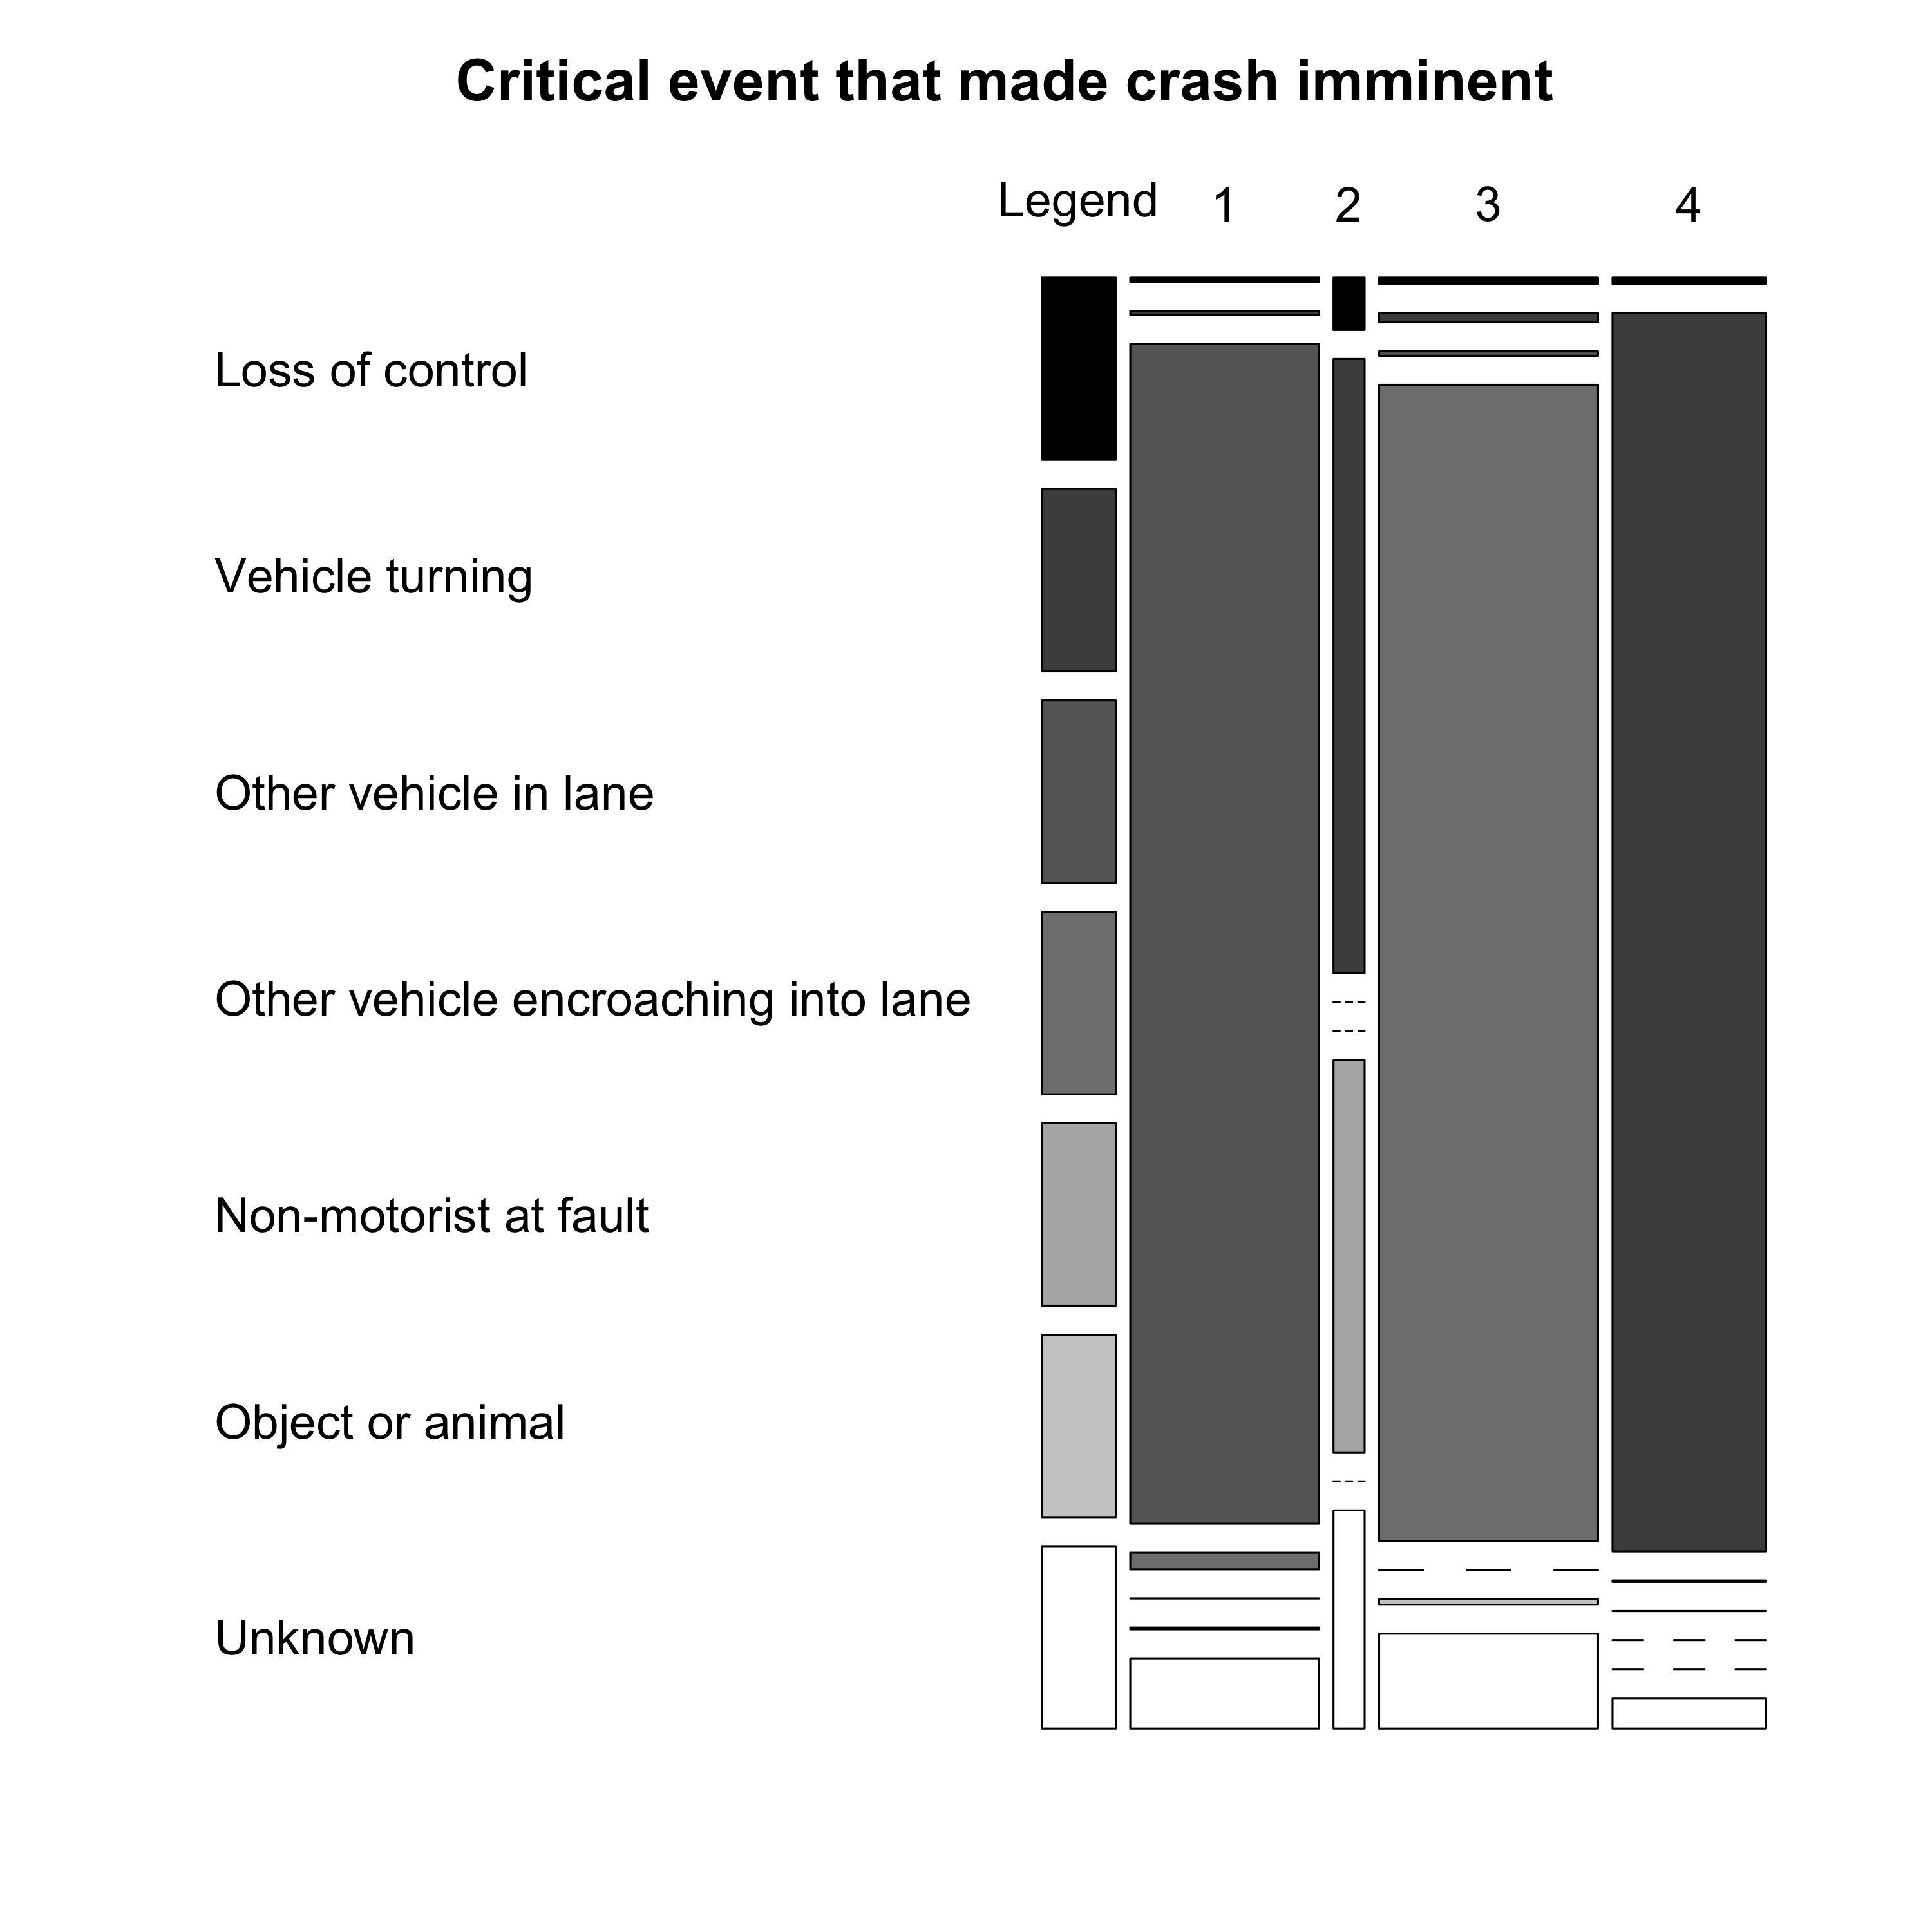
\includegraphics[width=1\linewidth]{crit_event_0509.png}
                \caption{2005--2009}
        \end{subfigure}%
        \begin{subfigure}{.5\textwidth}
%  \centering
                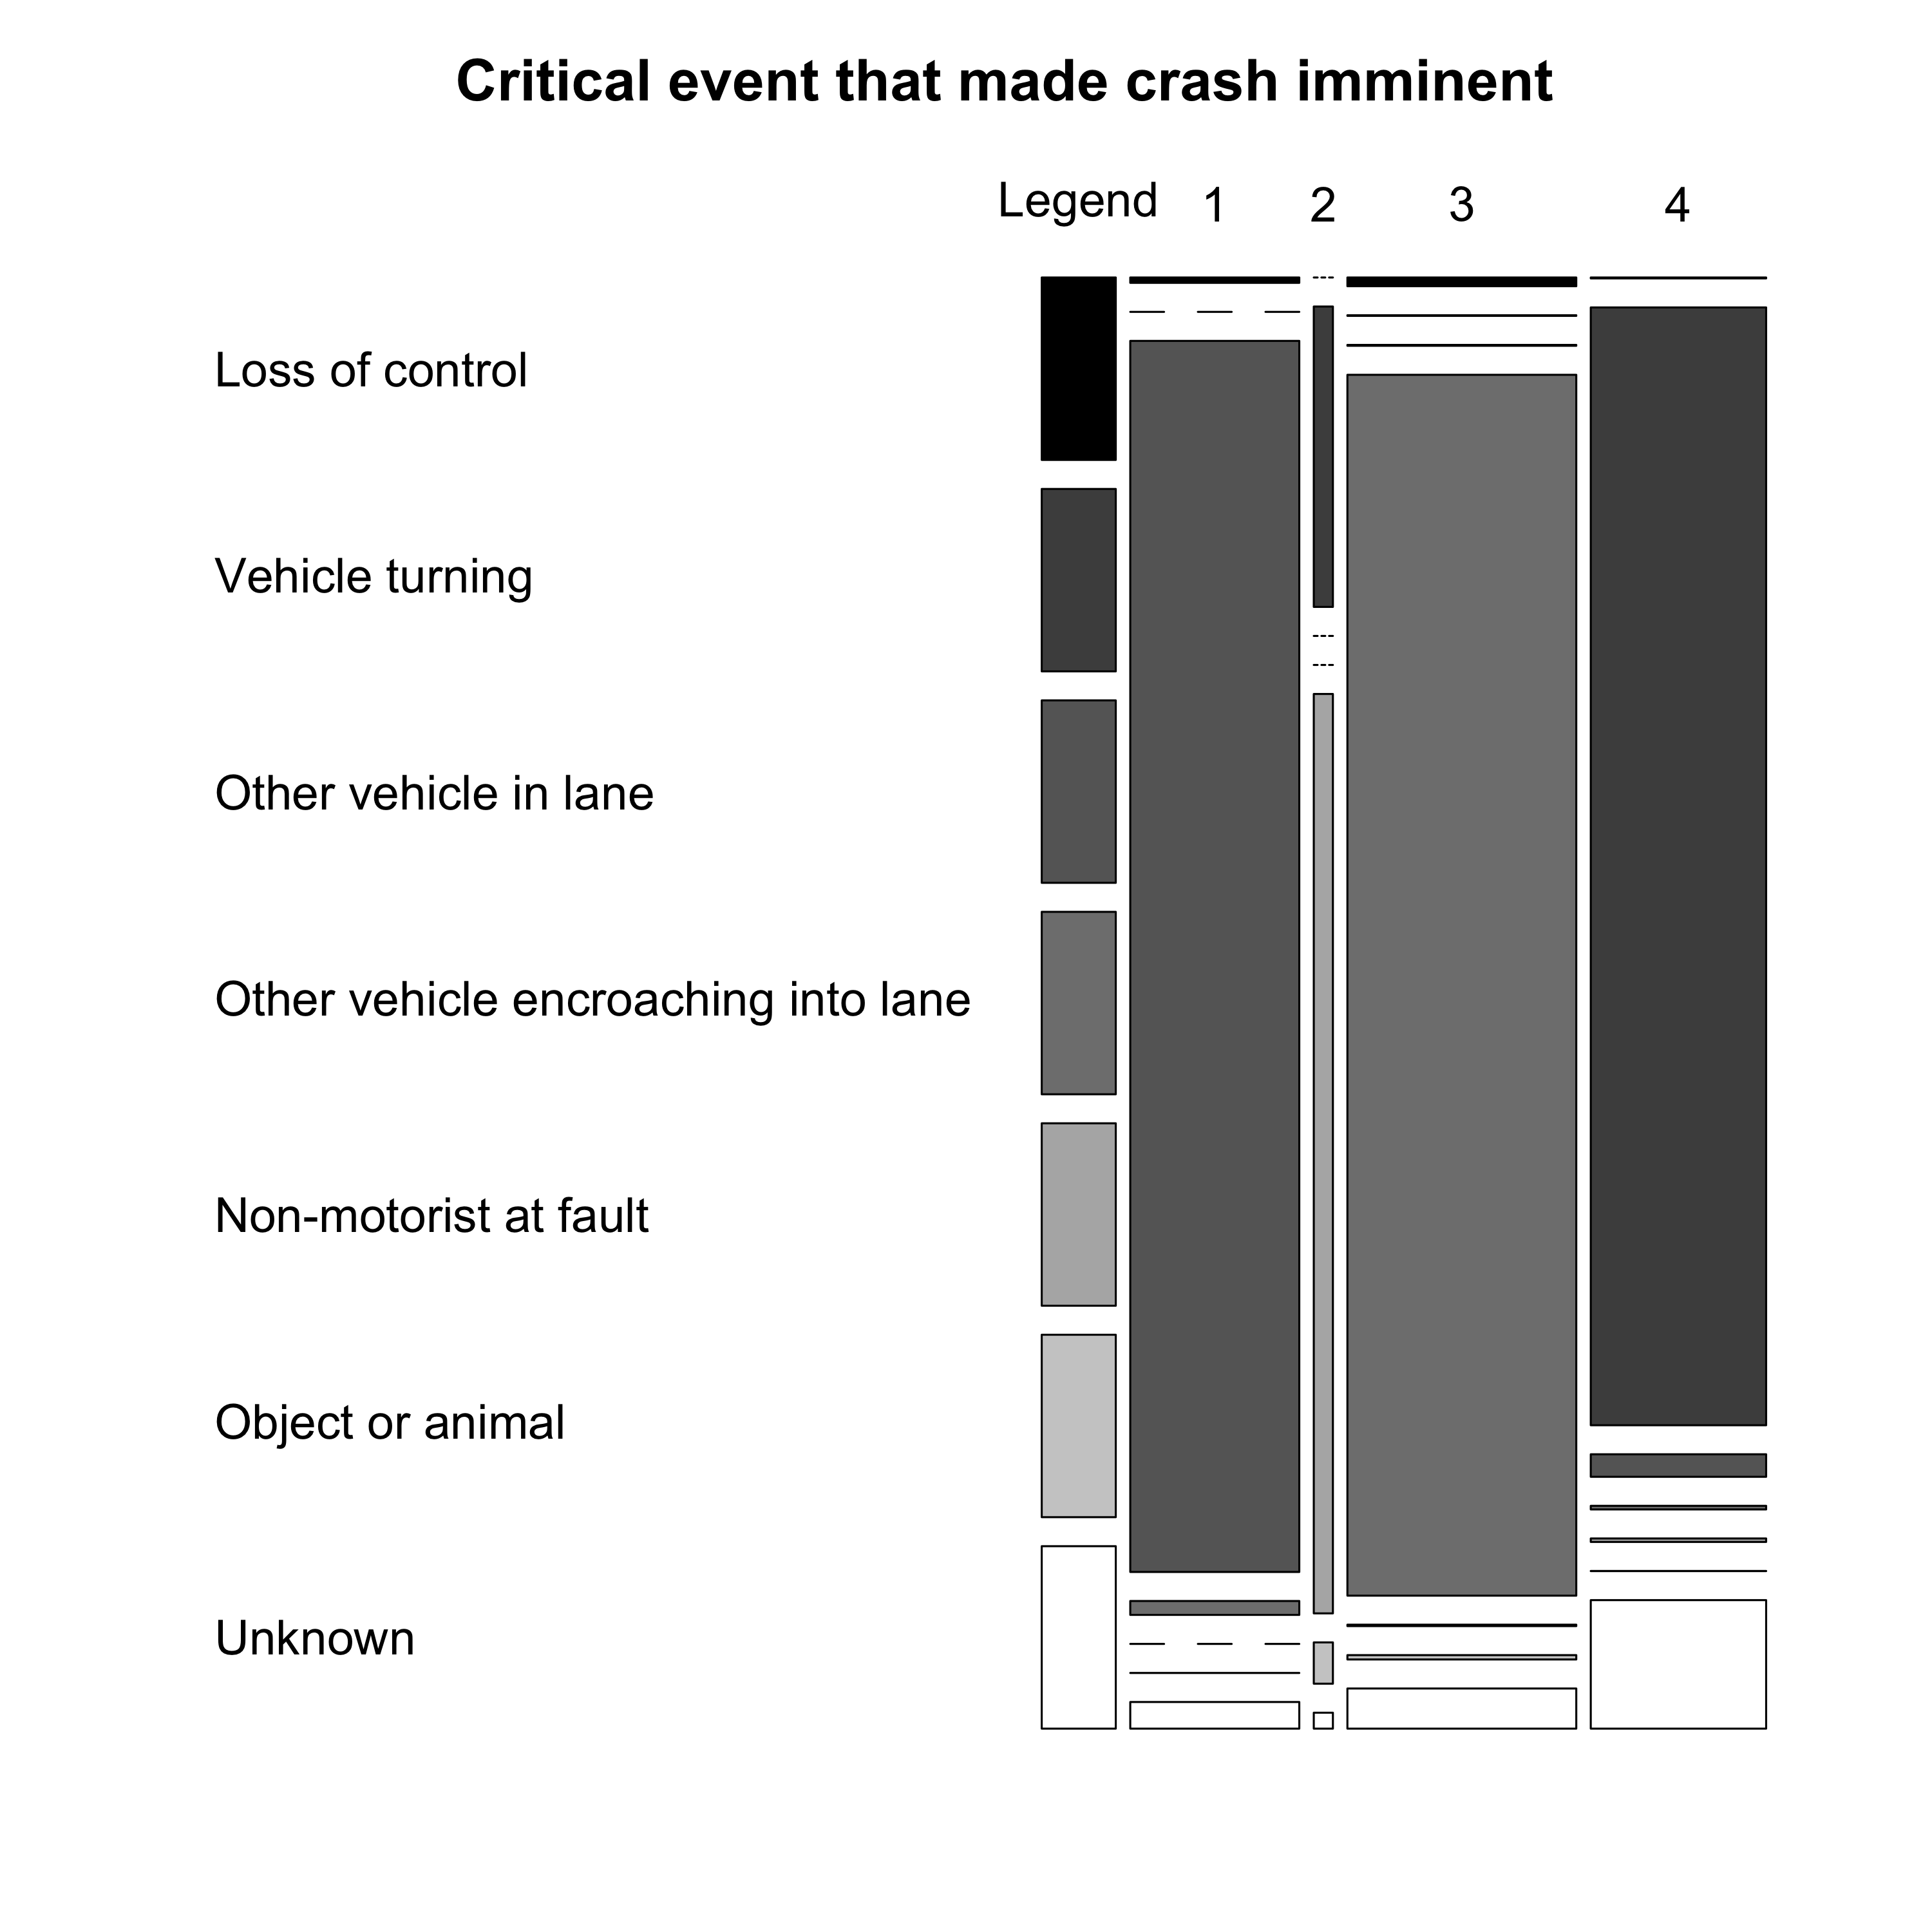
\includegraphics[width=1\linewidth]{crit_event.png}
                \caption{2010--2015}
        \end{subfigure}
        \caption{Mosaic plots giving the breakdown of the variable ``critical event that made the crash imminent'' for each of the four clusters.}
        \label{fig:clus12}
\end{figure}
%%%%%%%%%%%%%%%%%%%%%%%%%%%%%%%%%%%%%%%%%%%%%%%%%%%%%%%%%%%%%%%%%%%%%%%%%%%%%%%%%%%%

\noindent
\textbf{Cluster 3}:  Multi-vehicle crashes (86.1\% involving two vehicles, 13.9\% involving three or more vehicles), which happened largely due to the bus stopping (50.6\%), going straight (26.0\%) or decelerating (10.8\%). The cause of the crash was typically due to another vehicle being in the bus' lane (96.4\%). 27.1\% of the time, the bus driver was distracted. 51.7\% of the time, a school bus was involved. Most of the crashes happened during the daytime (89.9\%).
42.0\% of the time, the crash occurred at an intersection. In 31.0\% of the cases, the police found at least one driver of the other vehicles involved in the crash distracted and in 23.0\% of the cases, at least one of the other drivers was under the influence of alcohol, or drugs, or was impaired in some way. In 21.5\% of the cases, one of the other vehicles was a truck and in another 27.6\%, crashes involved an SUV, pickup truck, or van. 65.9\% of the crashes happened on roads with speed limit between 35--55 MPH, implying that these happened within a city or town and not on the highways.  48.7\% of the crashes happened where the road had no traffic control, and in 28.0\% of the cases, there was a traffic signal.
%%%%%%%%%%%%%%%%%%%%%%%%%%%%%%%%%%%%%%%%%%%%%%%%%%%%%%%%%%%%%%%%%%%%%%%%%%%%%%%%%%%%
\begin{figure}[t]
%\centering
        \begin{subfigure}{.5\textwidth}
%  \centering
                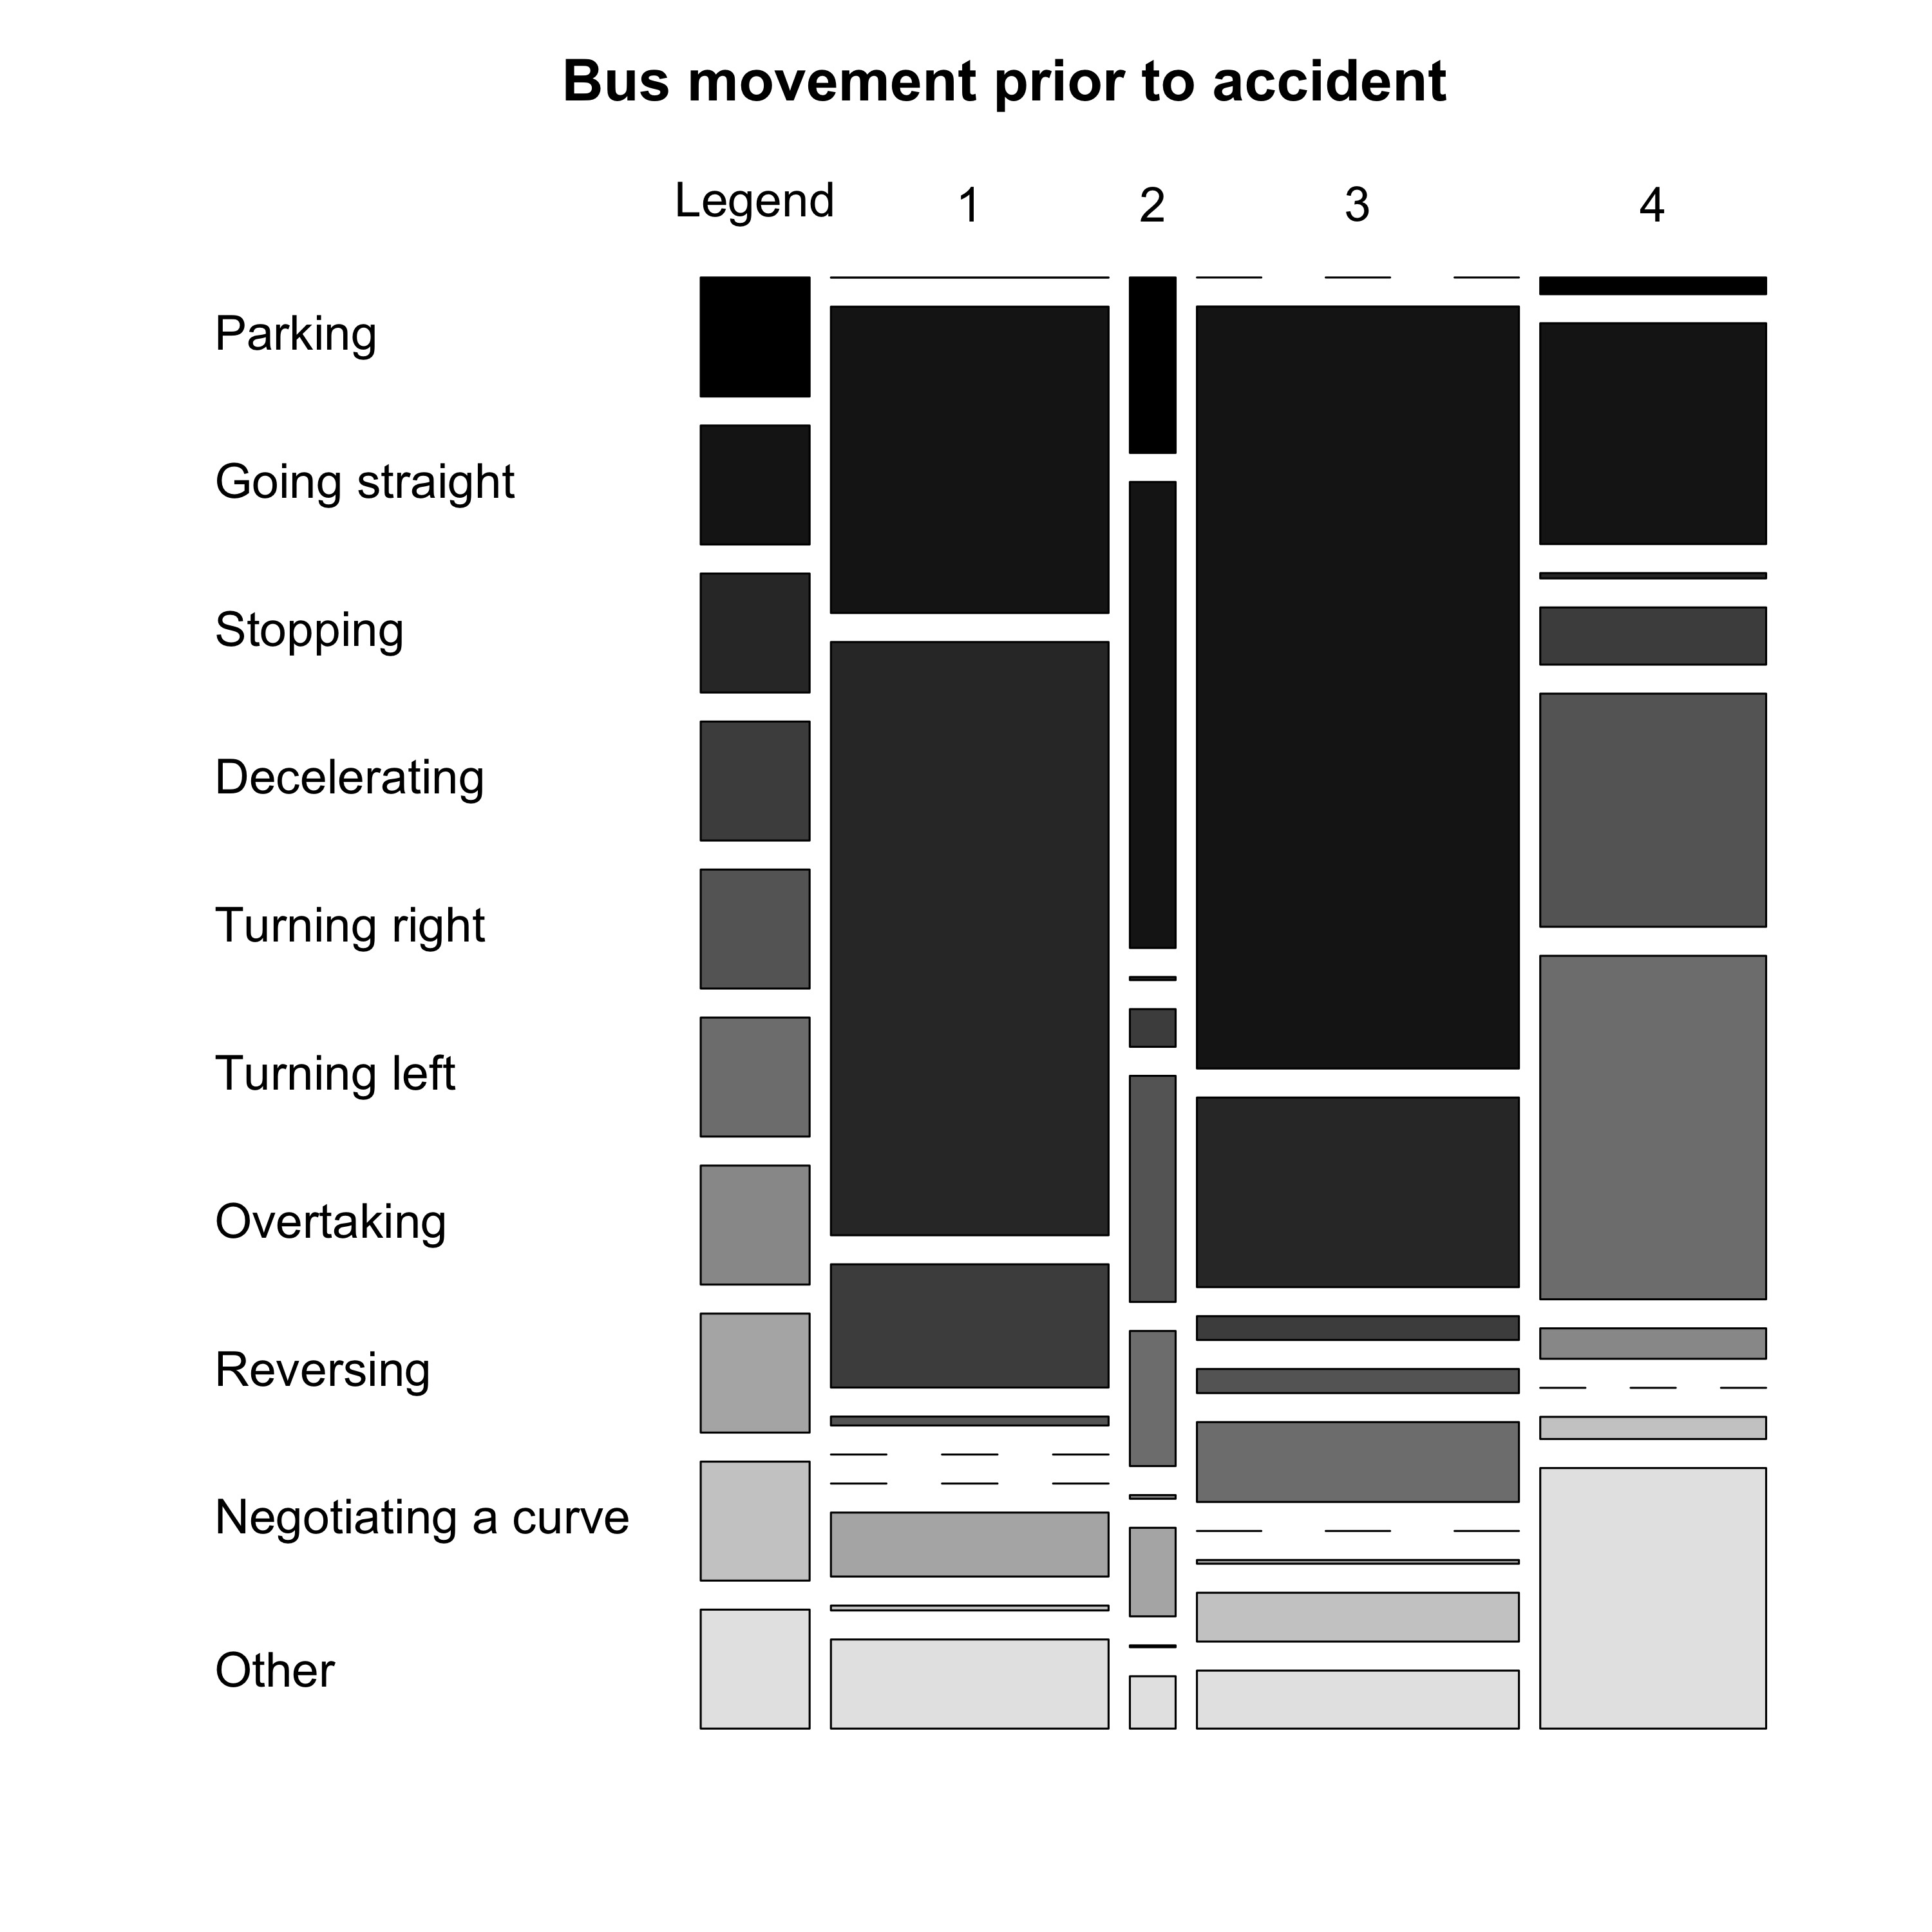
\includegraphics[width=1\linewidth]{bus_mov_0509.png}
                \caption{2005--2009}
        \end{subfigure}%
        \begin{subfigure}{.5\textwidth}
%  \centering
                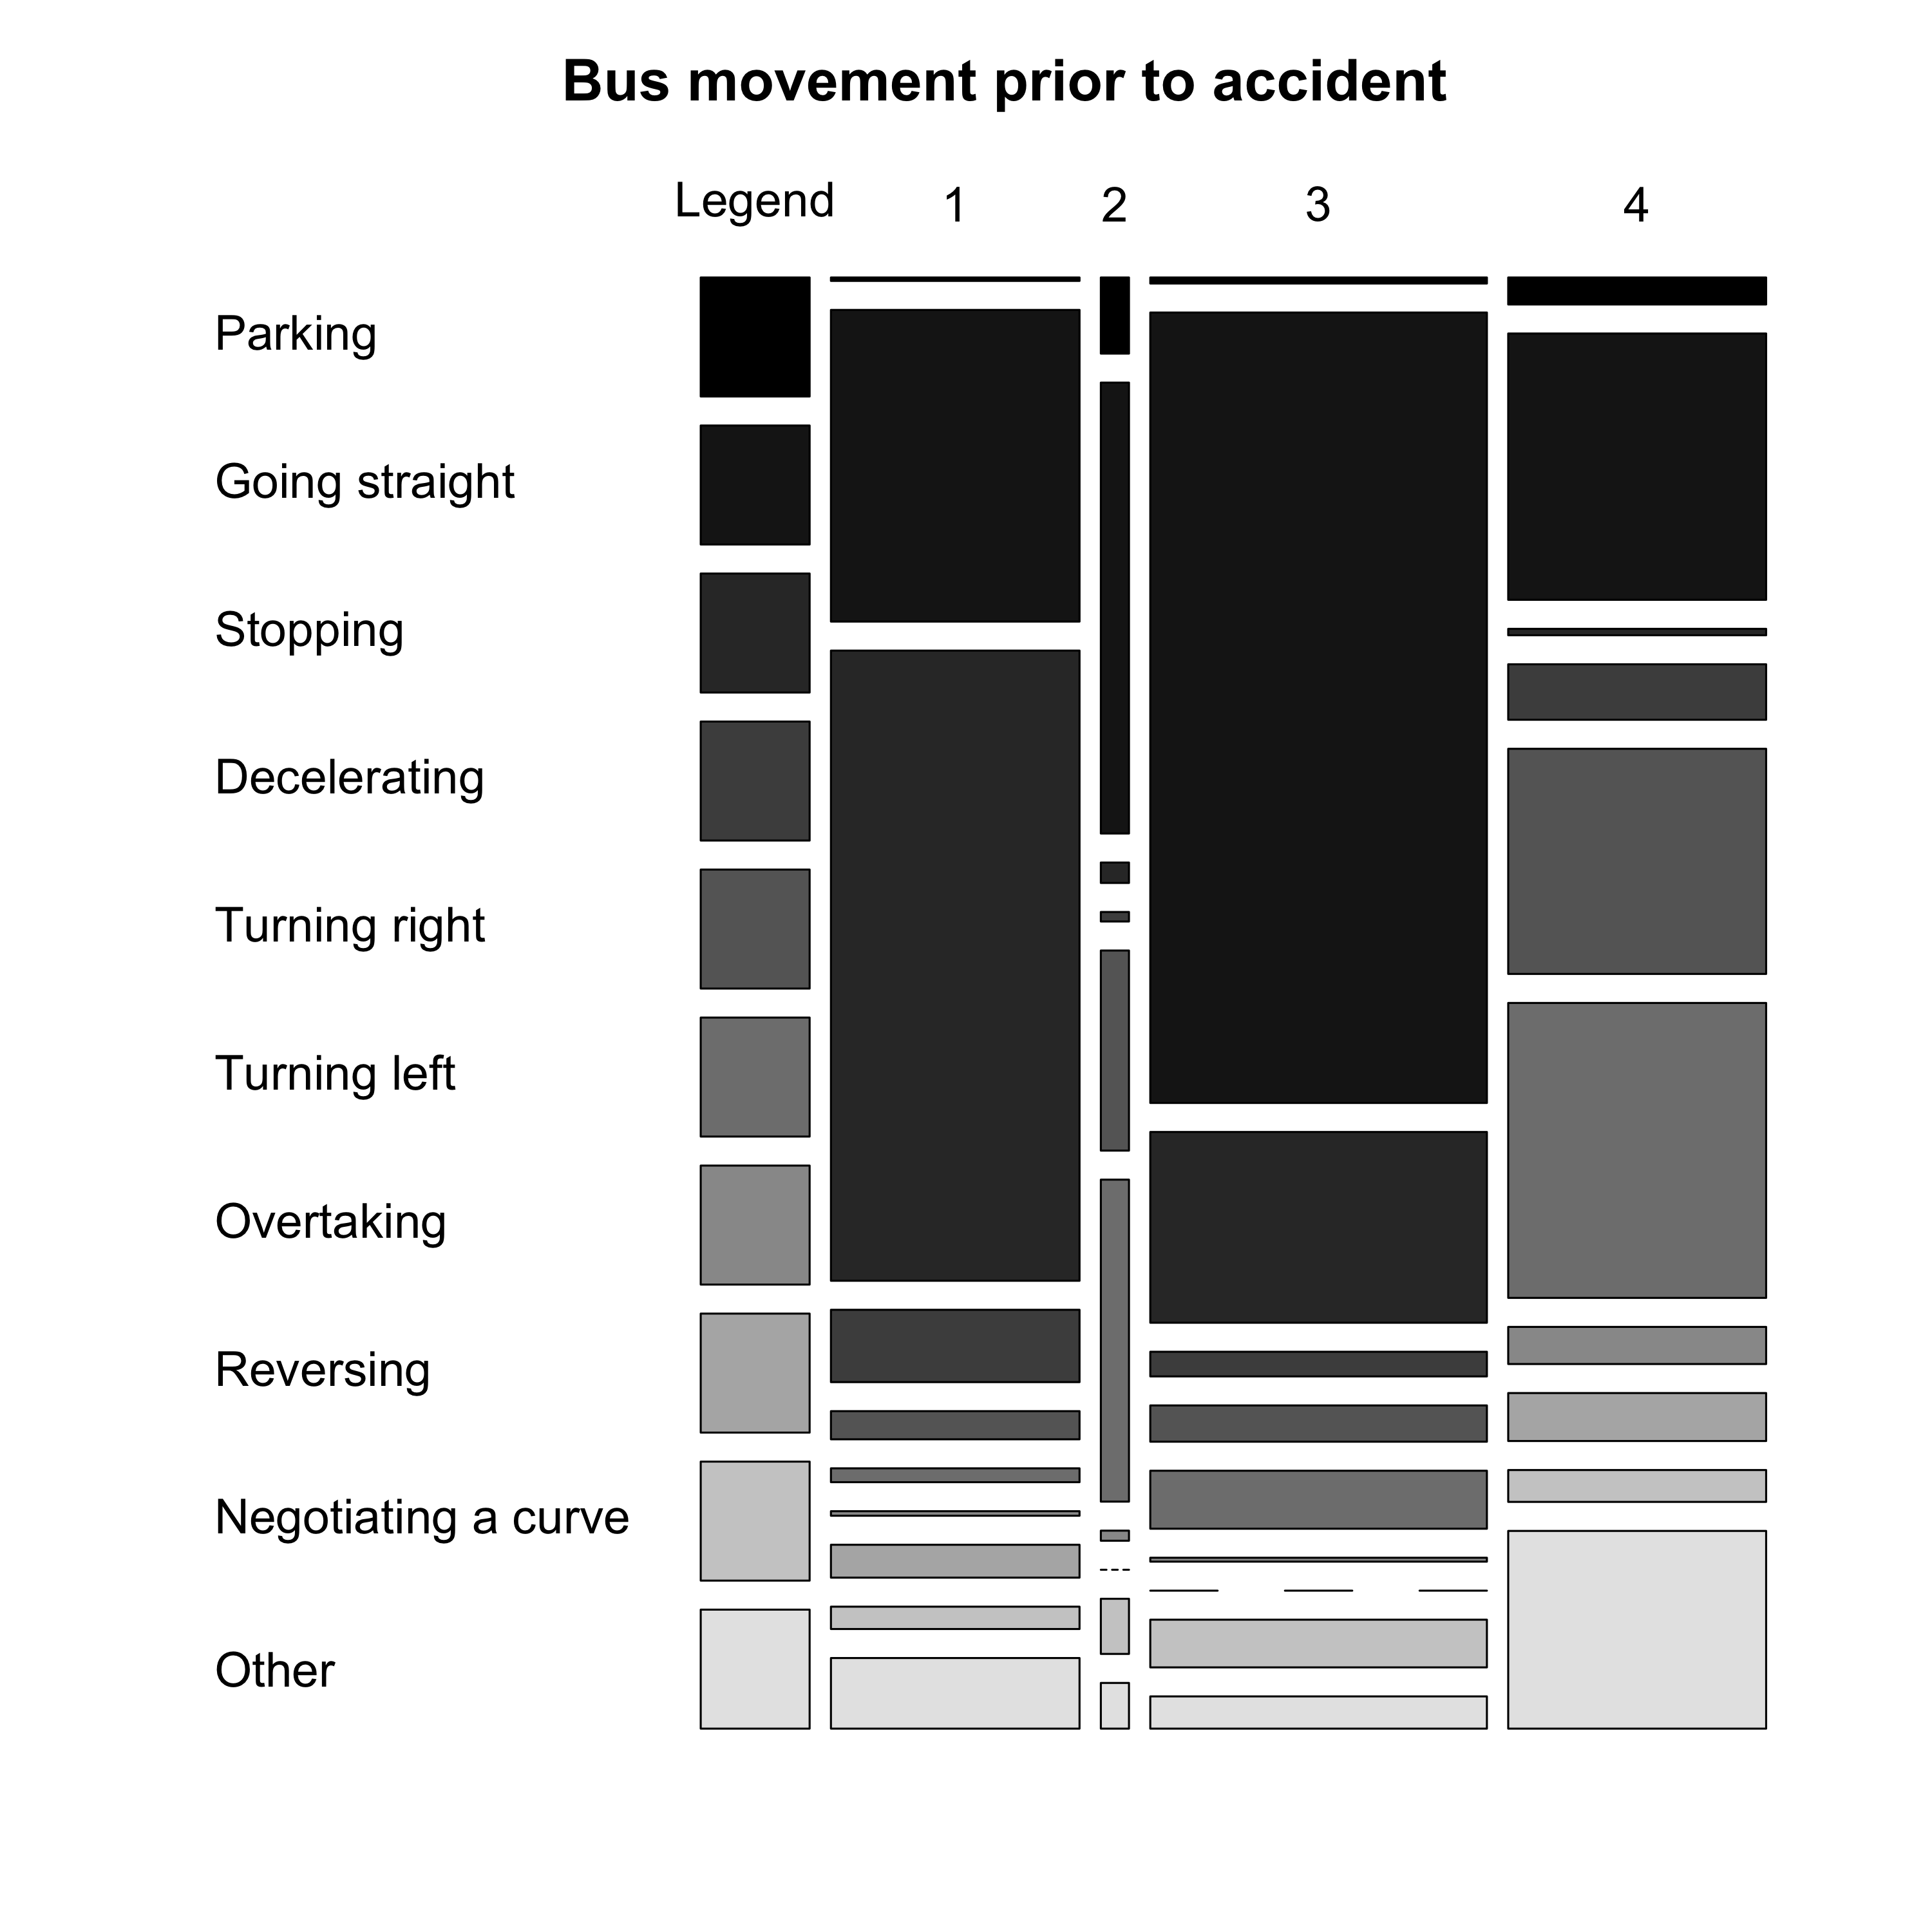
\includegraphics[width=1\linewidth]{bus_mov.png}
                \caption{2010--2015}
        \end{subfigure}
        \caption{Mosaic plots giving the breakdown of the variable ``bus movement prior to the crash'' for each of the four clusters.}
        \label{fig:clus4}
\end{figure} 
%%%%%%%%%%%%%%%%%%%%%%%%%%%%%%%%%%%%%%%%%%%%%%%%%%%%%%%%%%%%%%%%%%%%%%%%%%%%%%%%%%%%

\noindent
\textbf{Cluster 4}: Multi-vehicle crashes (98.9\% involving two vehicles) that happened when the bus was going straight (19.7\%), turning left (27.1\%) or making other movements such as passing/overtaking, merging, making a U-turn etc.   (20.5\%). The crash was primarily due to the bus trying to turn (90.7\%). In 32.1\% of the cases, the bus driver admitted to being distracted, and 35.4\% of the time, a school bus was involved. Most of the crashes happened on roadways with moderate to high speed limits (59.6\% on roads with 35--55 MPH and 33.8\% on roads with greater than 55 MPH). In only 4.9\% of the crashes was at least one of the other drivers involved distracted, and only 10.5\% of the cases involved at least one of the other drivers being impaired or under the influence. 63.0\% of the crashes happened at an intersection. 41.3\% of the crashes happened where the road had no traffic control, and in 33.6\% of the cases there was a traffic signal. 18.9\% of the cases involved a light or a heavy truck, and 29.9\% crashes involved an SUV, pickup truck, or van.

\noindent
Table \ref{table:tax1} summarizes the characteristics of the 2005--2009 bus crash clusters. 
%\begin{table}[H]
%\centering
%\resizebox{\textwidth}{!}{%
%\begin{tabular}{lllll}
%\rowcolor[HTML]{C0C0C0} 
%\multicolumn{1}{c}{\cellcolor[HTML]{C0C0C0}\textbf{Attribute}} & \multicolumn{1}{c}{\cellcolor[HTML]{C0C0C0}\textbf{Cluster 1}} & \multicolumn{1}{c}{\cellcolor[HTML]{C0C0C0}\textbf{Cluster 2}} & \multicolumn{1}{c}{\cellcolor[HTML]{C0C0C0}\textbf{Cluster 3}} & \multicolumn{1}{c}{\cellcolor[HTML]{C0C0C0}\textbf{Cluster 4}} \\
%\begin{tabular}[c]{@{}l@{}}Single vs. Multiple vehicles\\ (\textgreater85\%)\end{tabular} & Multiple & {\color[HTML]{9A0000} Single} & Multiple & Multiple \\
%Non-motorist involvement & 0.1\% & {\color[HTML]{680100} 99.5\%} & 0.4\% & 0\% \\
%Bus movement prior to crash & {\color[HTML]{9A0000} \begin{tabular}[c]{@{}l@{}}Stopping \\ (49.8\%)\end{tabular}} & {\color[HTML]{333333} \begin{tabular}[c]{@{}l@{}}Parking (14.7\%),\\ Going straight \\ (39.2\%), turning \\ left (19\%)\end{tabular}} & \begin{tabular}[c]{@{}l@{}}Going straight\\ (64\%), \\ stopping \\ (15.9\%)\end{tabular} & \begin{tabular}[c]{@{}l@{}}Turning left\\ (19.6\%), \\ overtaking \\ (28.9\%), \\ other (21.9\%)\end{tabular} \\
%\begin{tabular}[c]{@{}l@{}}Critical event that made the \\ crash imminent\end{tabular} & \begin{tabular}[c]{@{}l@{}}In another \\ vehicle's \\ lane (92.3\%)\end{tabular} & \begin{tabular}[c]{@{}l@{}}Vehicle turning\\ (48.1\%), non-\\ motorist \\ encroaching into\\ lane (30.7\%)\end{tabular} & \begin{tabular}[c]{@{}l@{}}Encroaching\\ in another \\ vehicle's \\ lane (90.5\%)\end{tabular} & \begin{tabular}[c]{@{}l@{}}Vehicle \\ turning \\ (96.9\%)\end{tabular} \\ 
%Bus driver distracted & 27.4\% & 33.9\% & 20.2\% & 31.8\% \\ \\
%\begin{tabular}[c]{@{}l@{}}Other vehicle's driver or the \\ non-motorist charged with \\ alcohol/drug/impairment \\ related offense\end{tabular} & 22.1\% & {\color[HTML]{9A0000} 4.7\%} & 20.5\% & 10.5\% \\
%Was a school bus involved? & {\color[HTML]{9A0000} 51.8\%} & 39.8\% & 39.9\% & 32.2\% \\ \\
%\begin{tabular}[c]{@{}l@{}}Daylight condition - was there\\ sufficient light?\end{tabular} & 90.1\% & 89.5\% & 86.1\% & 81.4\% \\ \\
%\begin{tabular}[c]{@{}l@{}}Did the accident happen at an\\ intersection?\end{tabular} & 40.8\% & 44.3\% & 49.6\% & {\color[HTML]{9A0000} 66.9\%} \\ \\
%Bus driver (male)? & 56.9\% & 55.8\% & 62.7\% & 65.7\% \\ \\
%Light/ heavy truck involvement & 21.6\% & {\color[HTML]{9A0000} 0.1\%} & 22.5\% & 19.9\% \\ \\
%\begin{tabular}[c]{@{}l@{}}Was the other driver/ \\ non motorist distracted?\end{tabular} & 30.6\% & {\color[HTML]{9A0000} 100\%} & 24.9\% & {\color[HTML]{9A0000} 4.9\%} \\ \\
%\begin{tabular}[c]{@{}l@{}}Was there a pick-up truck/ van/\\ SUV involved?\end{tabular} & 28.4\% & 24.8\% & 27.1\% & {\color[HTML]{9A0000} 0\%} \\ \\
%Single lane vs. multiple lanes & {\color[HTML]{9A0000} 22.4\%} & 35.3\% & 31.1\% & 36.7\%
%\end{tabular}%
%}
%\caption{Taxonomy of crashes 2005 - 2009}
%\label{table: tax1}
%\end{table}
%%%%%%%%%%%%%%%%%%%%%%%%%%%%%%%%%%%%%%%%%%%%%%%%%%%%%%%%%%%%%%%%%%%%%%%%%%%%%%%%%%%%
\begin{figure}[t]
%\centering
        \begin{subfigure}{.5\textwidth}
%  \centering
                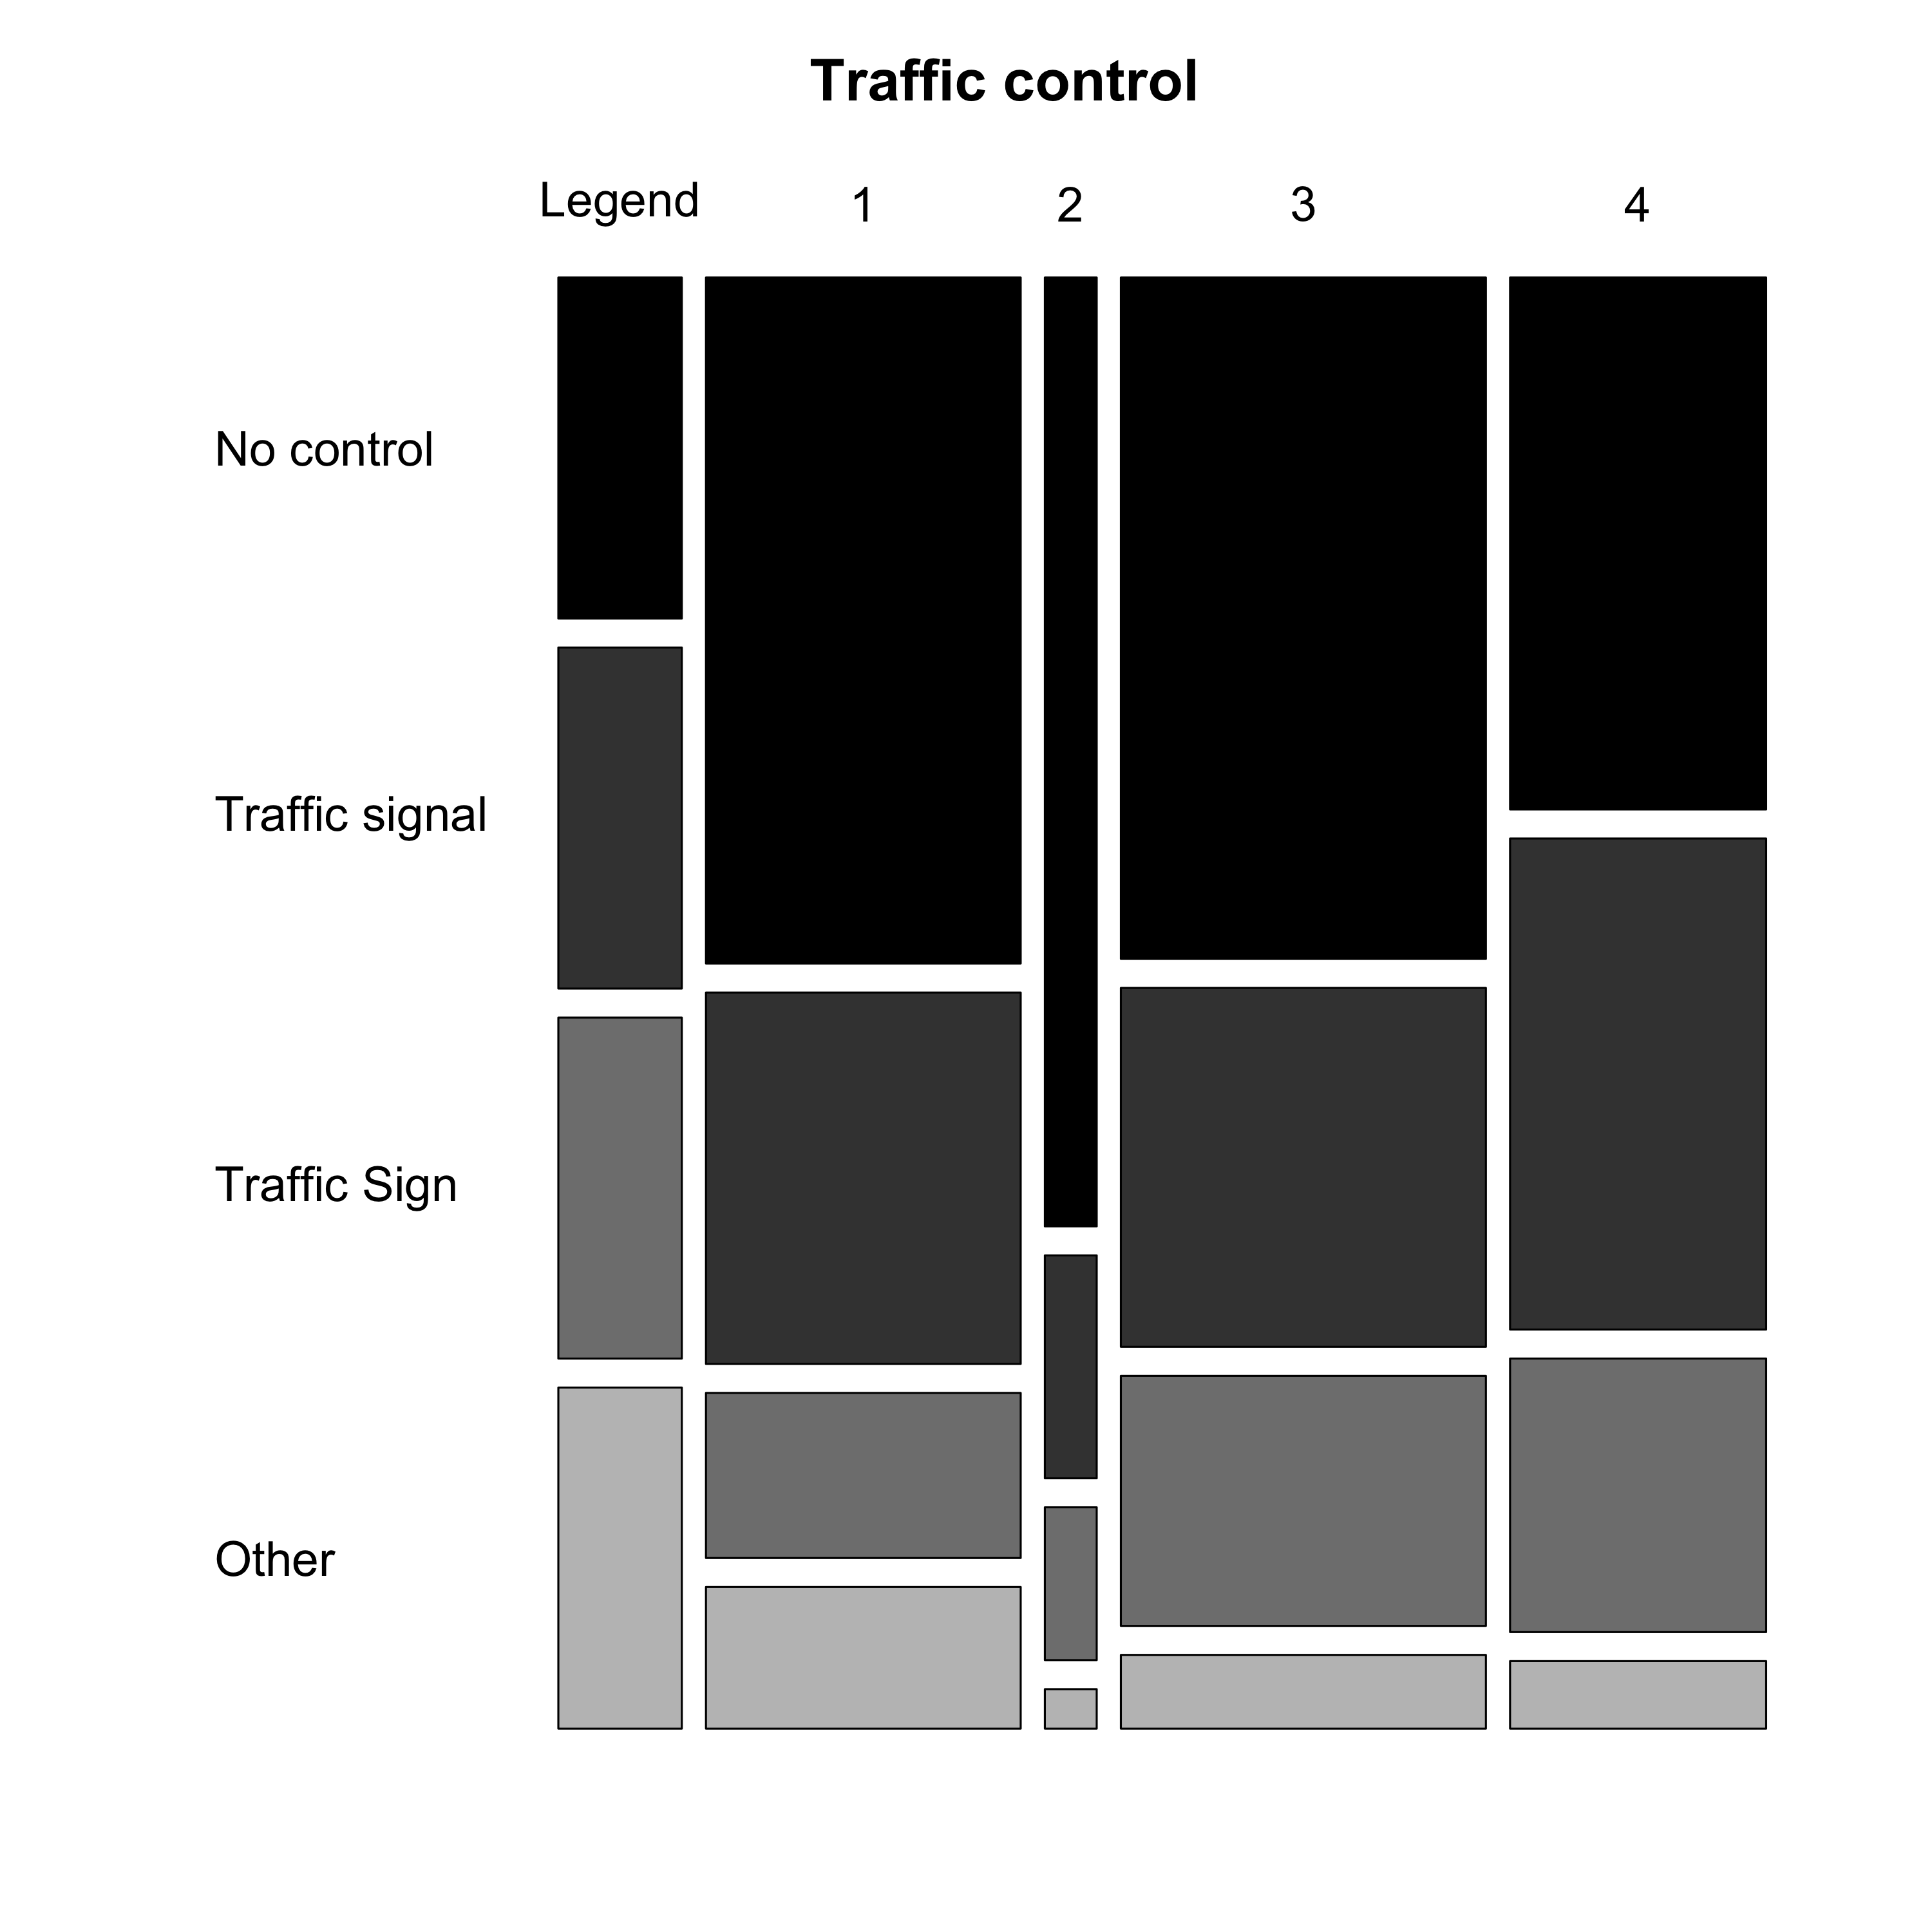
\includegraphics[width=1\linewidth]{traf_control_0509.png}
                \caption{2005--2009}
        \end{subfigure}%
        \begin{subfigure}{.5\textwidth}
%  \centering
                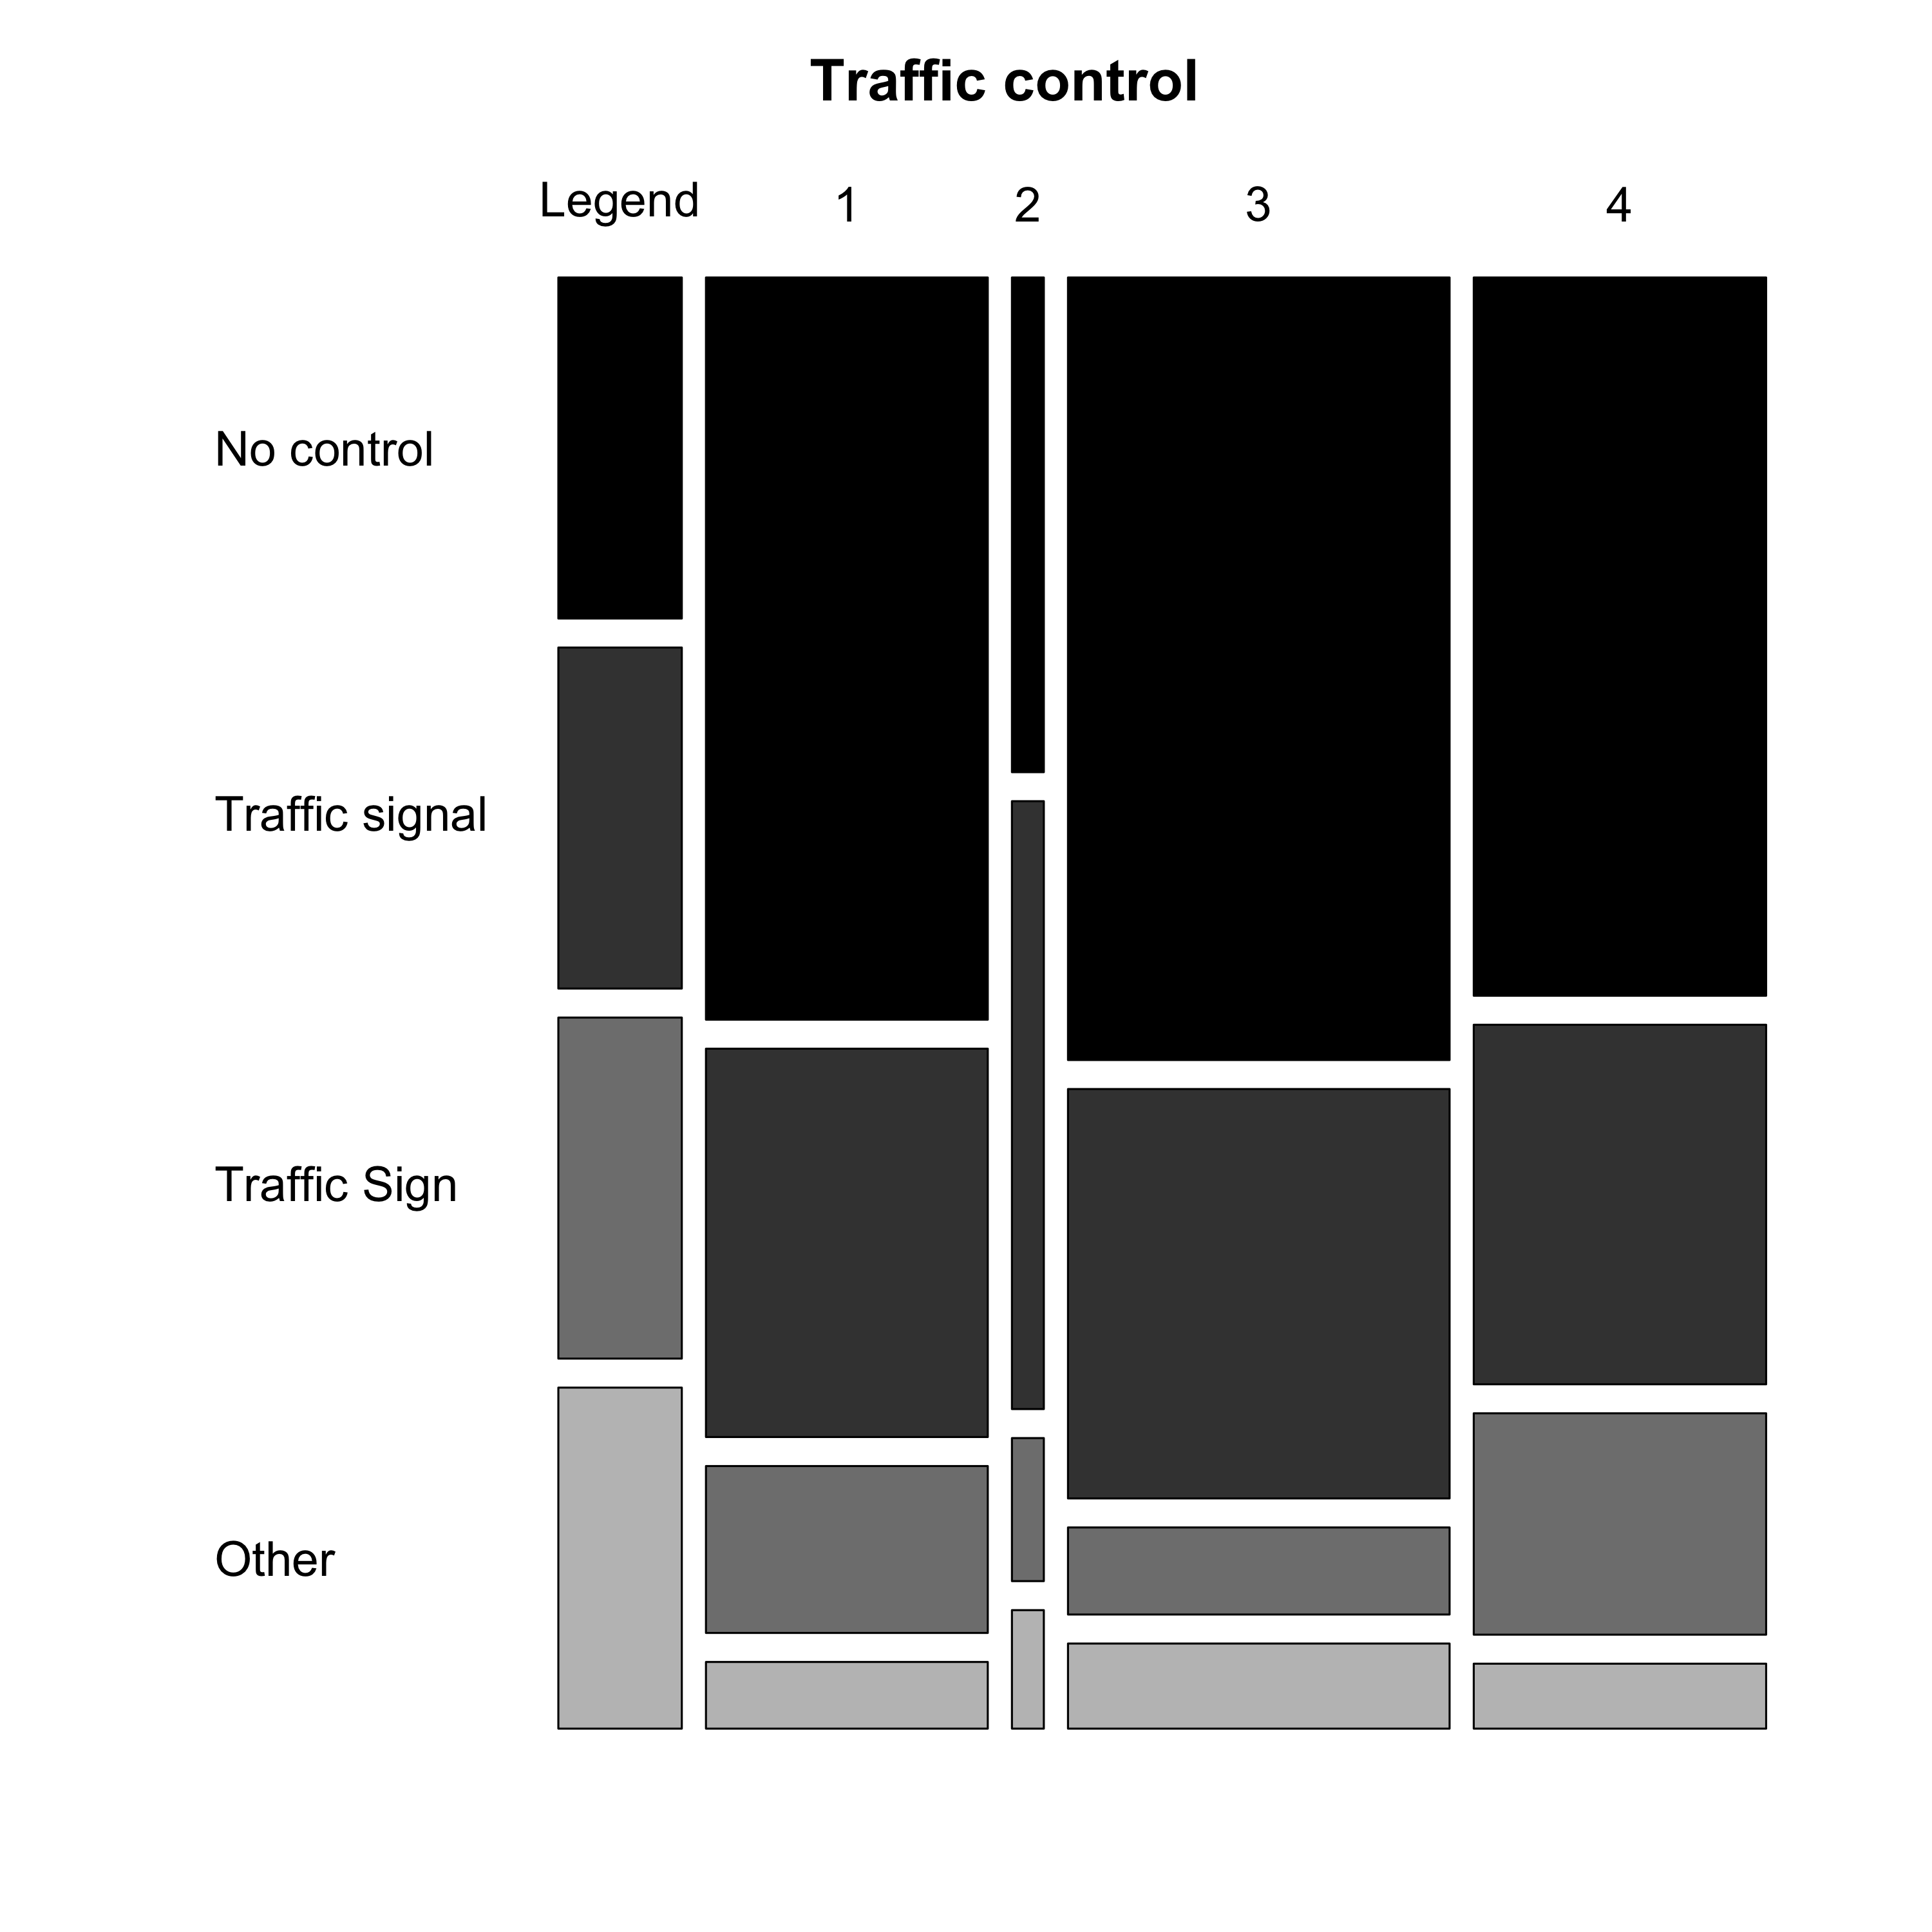
\includegraphics[width=1\linewidth]{traf_control.png}
                \caption{2010--2015}
        \end{subfigure}
        \caption{Mosaic plots giving the breakdown of the variable ``traffic control devices applicable to the bus at the time of the accident'' for each of the four clusters.}
        \label{fig:clus8}
\end{figure}
%%%%%%%%%%%%%%%%%%%%%%%%%%%%%%%%%%%%%%%%%%%%%%%%%%%%%%%%%%%%%%%%%%%%%%%%%%%%%%%%%%%%

%%%%%%%%%%%%%%%%%%%%%%%%%%%%%%%%%%%%%%%%%%%%%%%%%%%%%%%%%%%%%%%%%%%%%%%%%%%%%%%%%%%%
\begin{figure}[t]
%\centering
        \begin{subfigure}{.5\textwidth}
%  \centering
                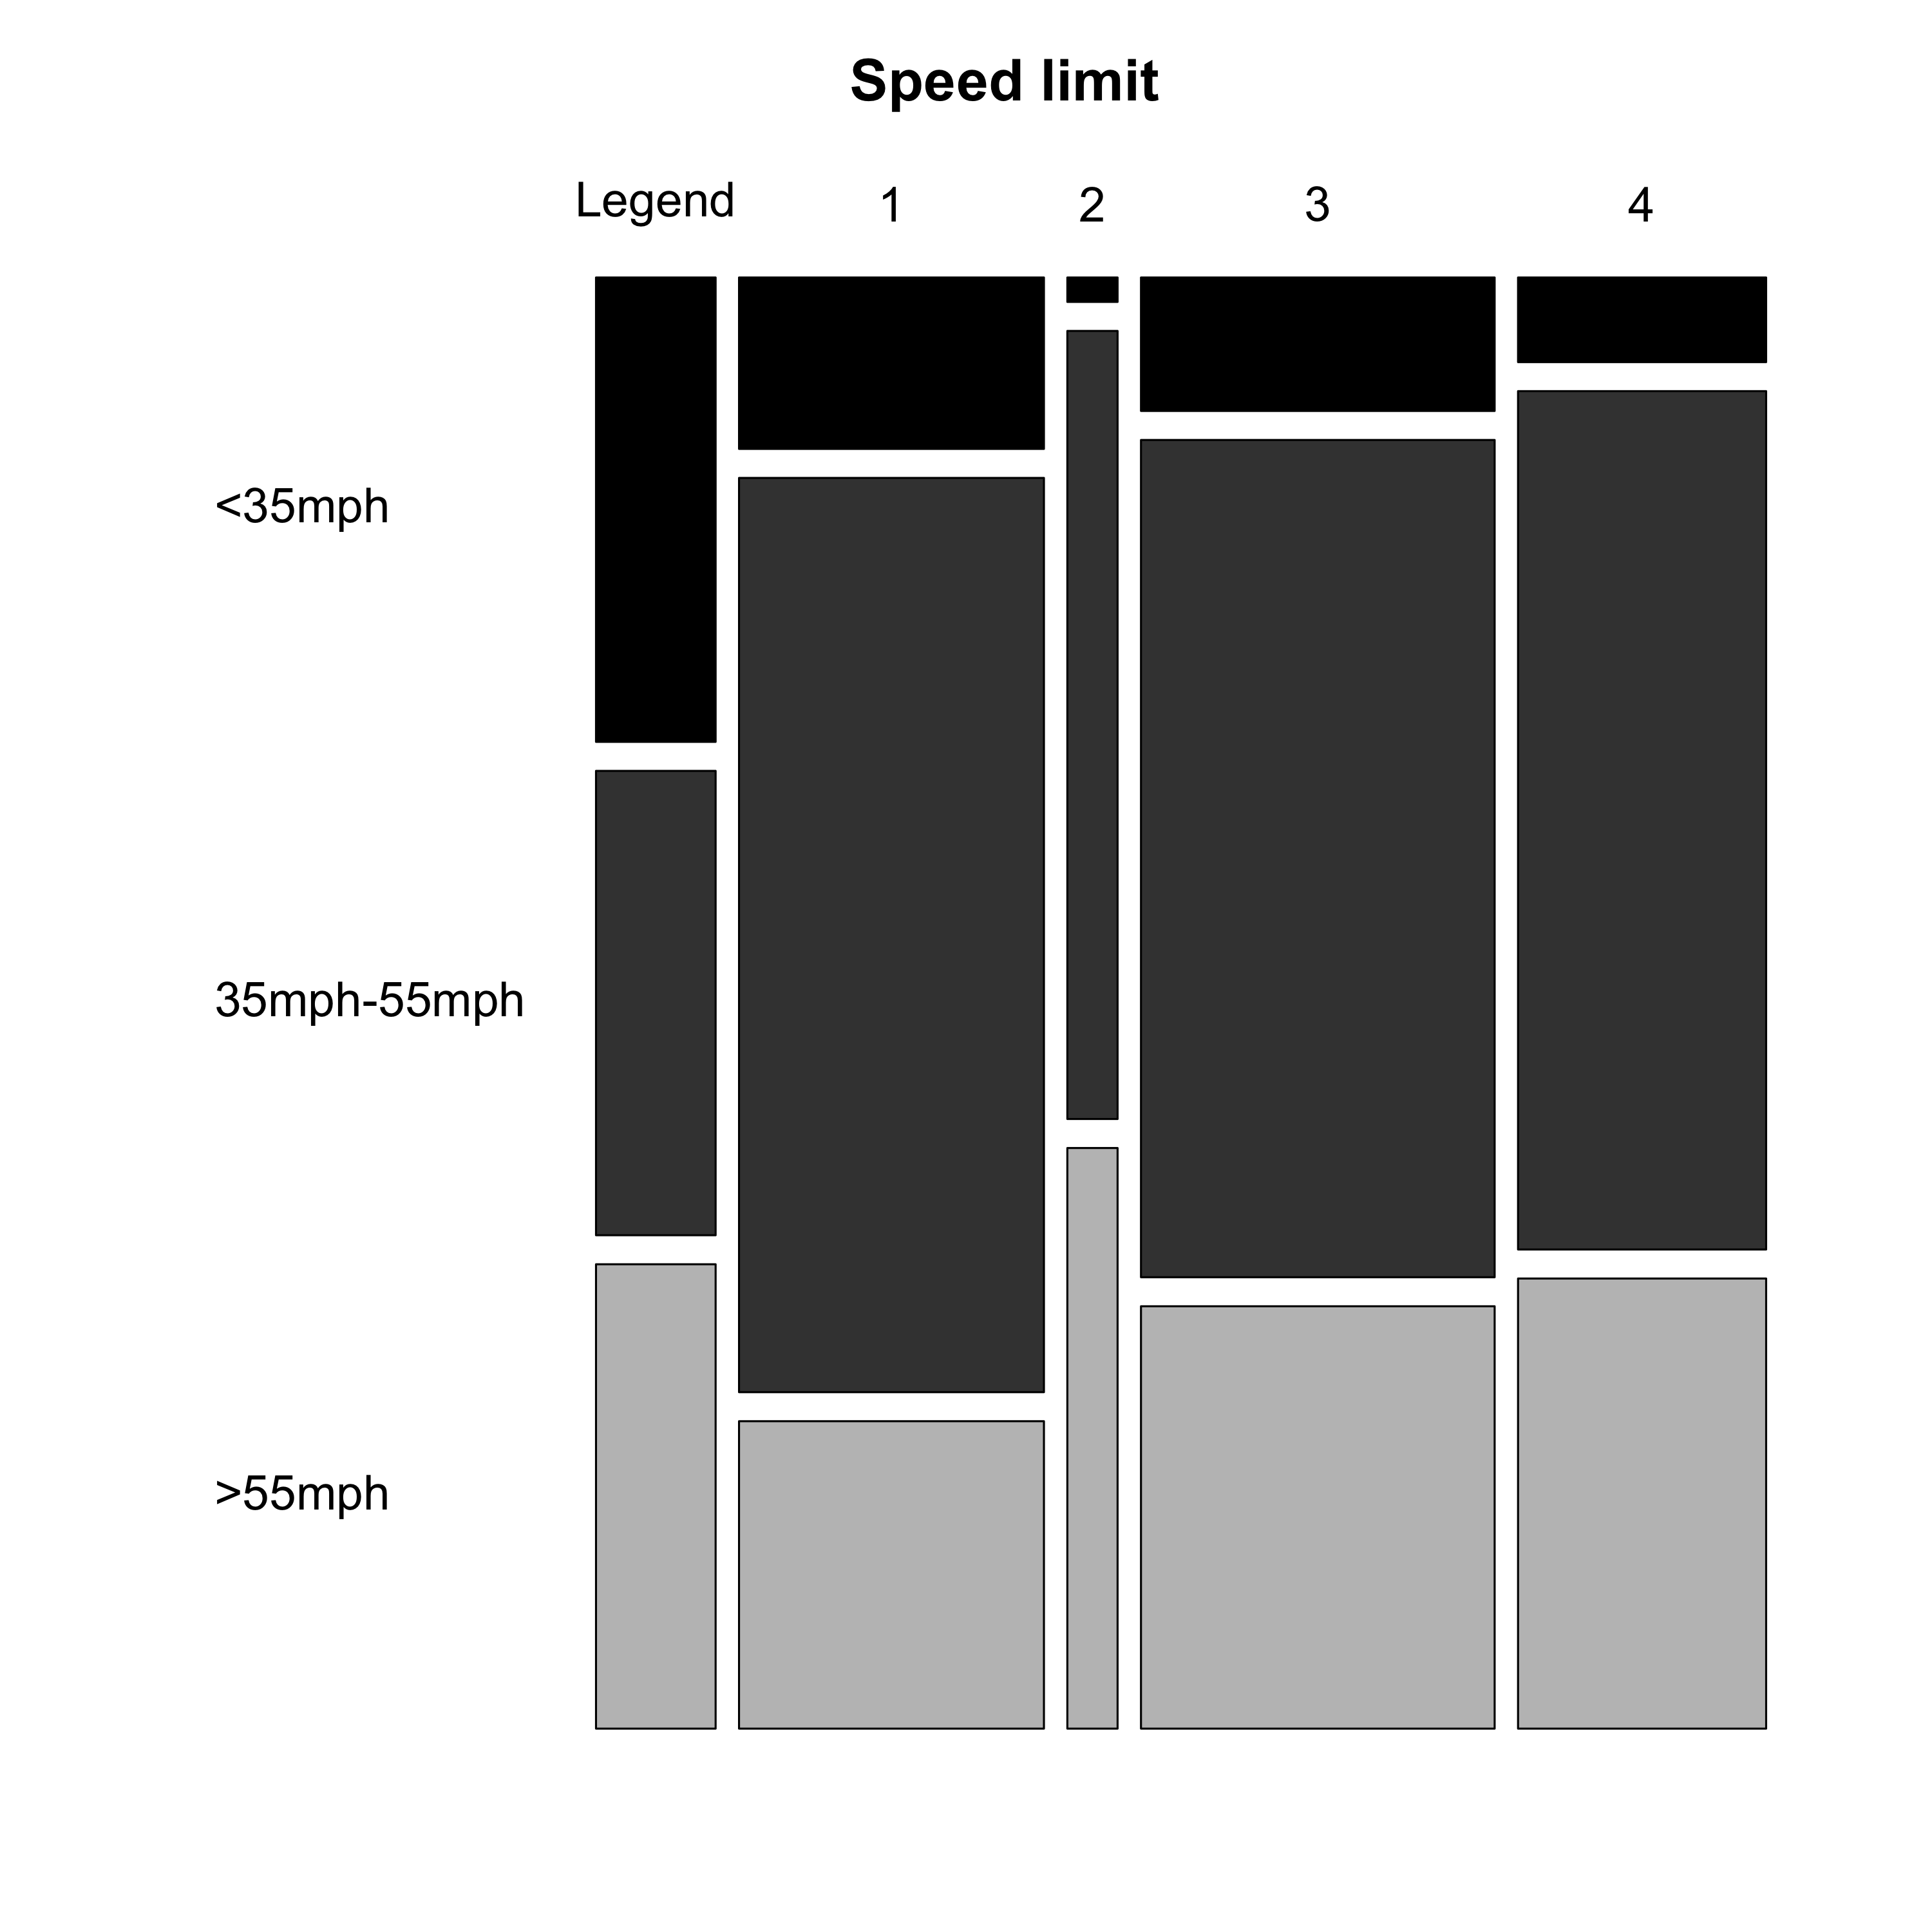
\includegraphics[width=1\linewidth]{spd_lim_0509.png}
                \caption{2005--2009}
        \end{subfigure}%
        \begin{subfigure}{.5\textwidth}
%  \centering
                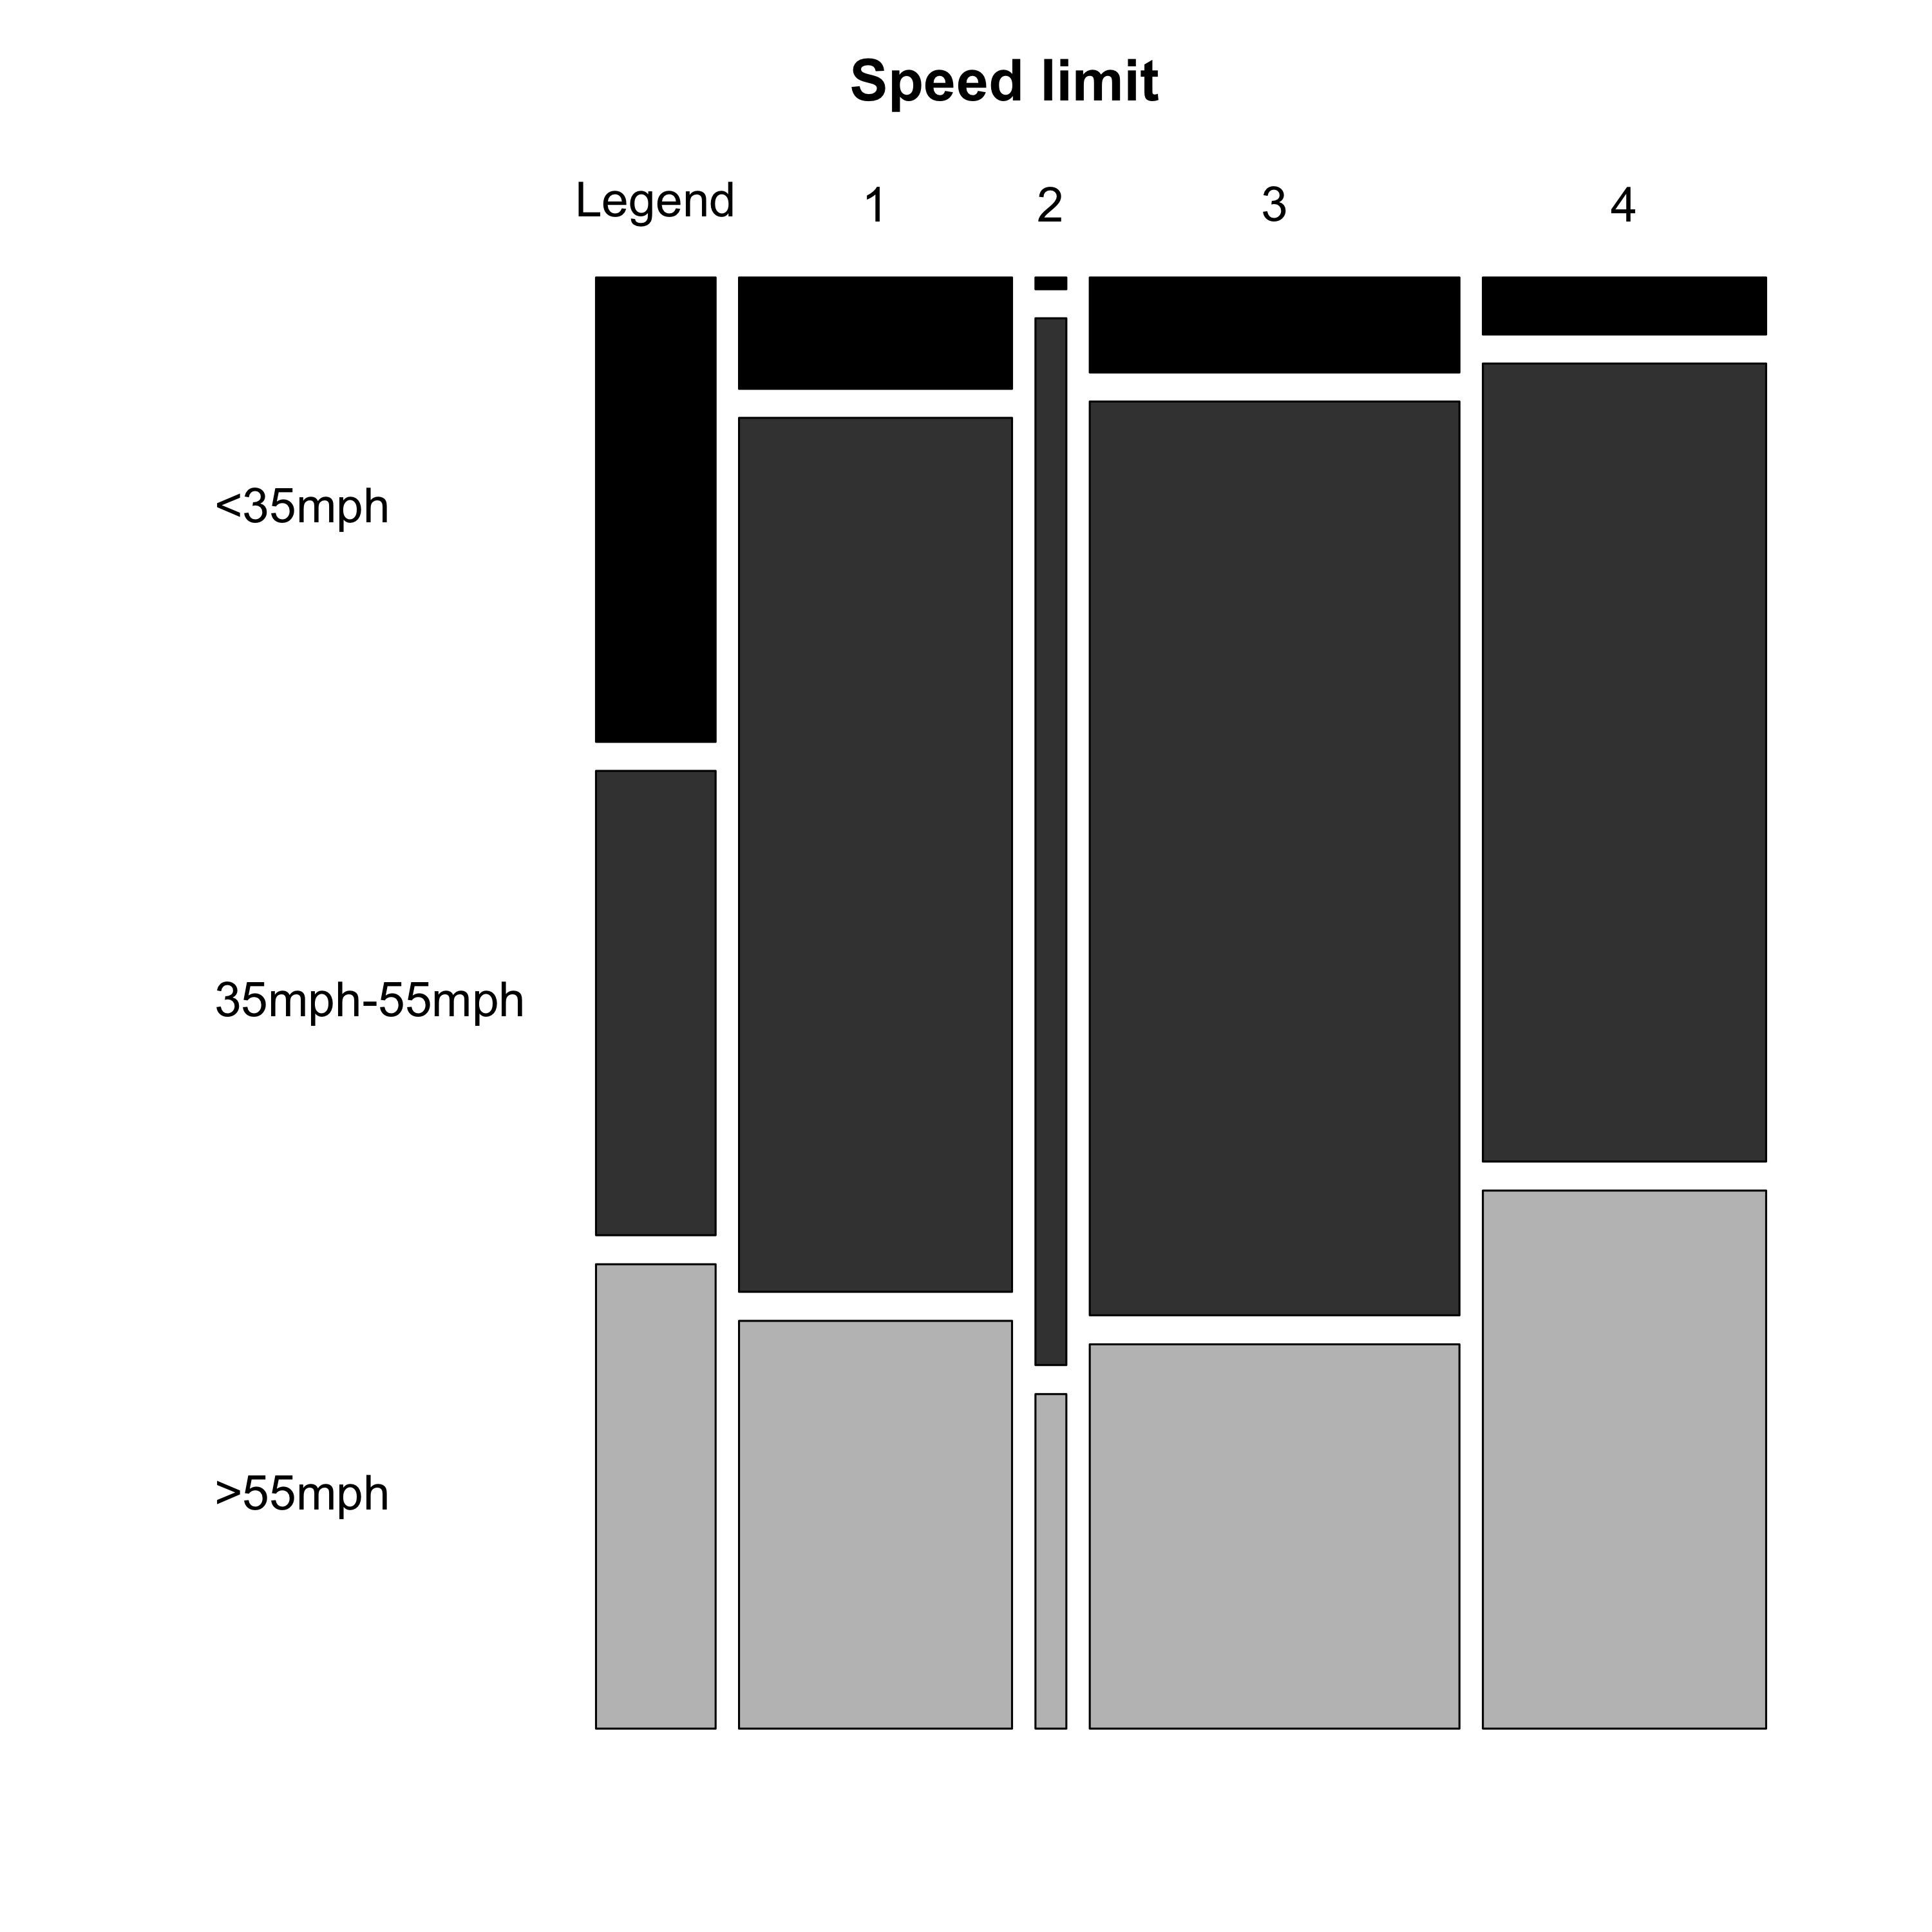
\includegraphics[width=1\linewidth]{spd_lim.png}
                \caption{2010--2015}
        \end{subfigure}
        \caption{Mosaic plots giving the breakdown of the variable ``speed limit of the traffic way where the accident occurred'' for each of the four clusters.}
 \label{fig:clus6}
\end{figure}
%%%%%%%%%%%%%%%%%%%%%%%%%%%%%%%%%%%%%%%%%%%%%%%%%%%%%%%%%%%%%%%%%%%%%%%%%%%%%%%%%%%%

%%%%%%%%%%%%%%%%%%%%%%%%%%%%%%%%%%%%%%%%%%%%%%%%%%%%%%%%%%%%%%%%%%%%%%%%%%%%%%%%%%%%
\begin{figure}[t]
%\centering
        \begin{subfigure}{.5\textwidth}
 \centering
                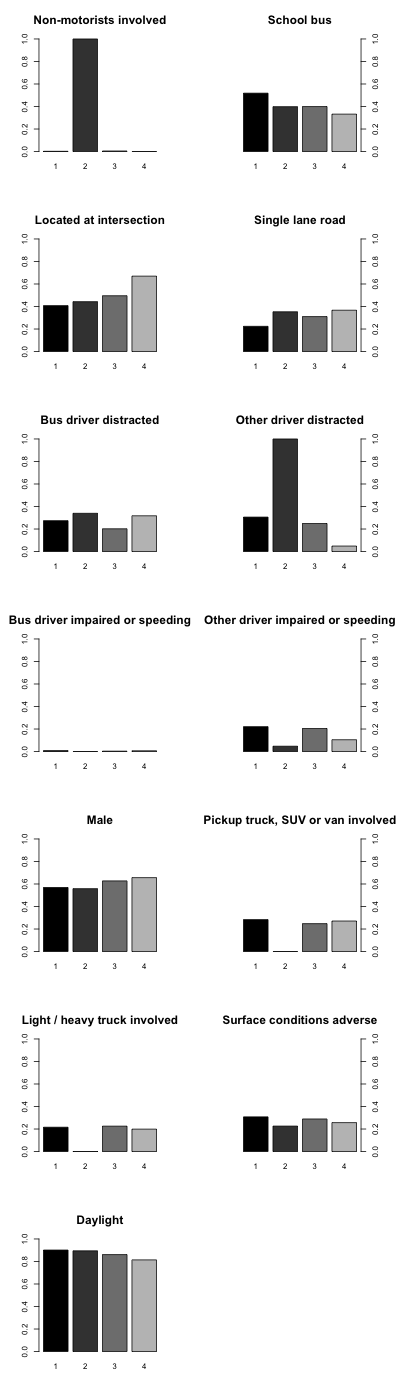
\includegraphics[width=.8\linewidth]{binary_proportions_scaled_0509.png}
                \caption{2005--2009}
        \end{subfigure}%
        \begin{subfigure}{.5\textwidth}
 \centering
                  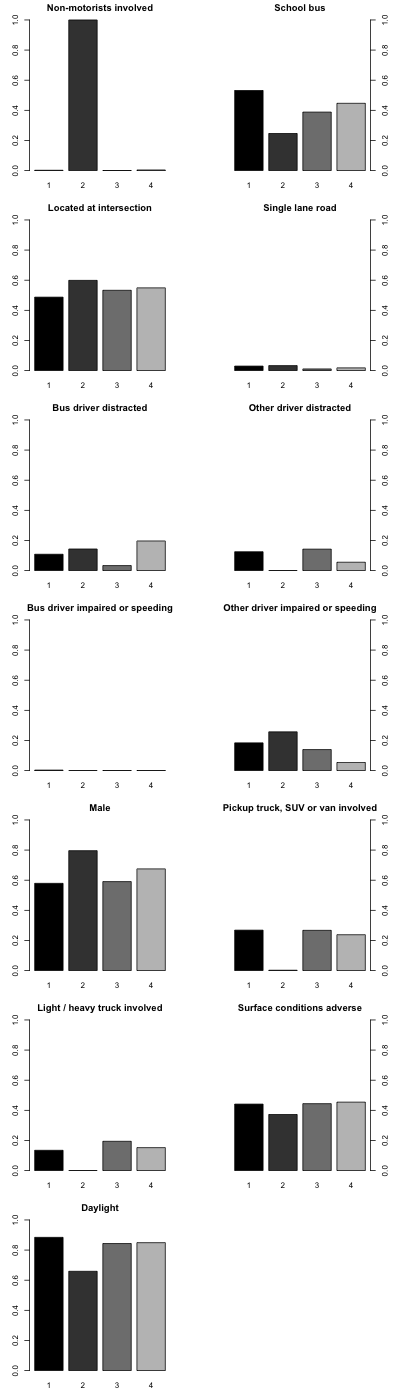
\includegraphics[width=.8\linewidth]{binary_proportions_scaled.png}
                  \caption{2010--2015}
        \end{subfigure}
        \caption{Observed proportions for binary response variables for each of the four clusters.}
 \label{fig:clus2}
\end{figure}
%%%%%%%%%%%%%%%%%%%%%%%%%%%%%%%%%%%%%%%%%%%%%%%%%%%%%%%%%%%%%%%%%%%%%%%%%%%%%%%%%%%%

%%%%%%%%%%%%%%%
\begin{table}[t]
        \centering
        \caption{Taxonomy of crashes, 2005--2009.}
        \label{table:tax1}
        \resizebox{\textwidth}{!}{
        \begin{tabular}{@{}lllll@{}}
        \toprule
Characteristic                    & Cluster 1                       & Cluster 2                     & Cluster 3                    & Cluster 4 \\ \midrule
Single vs. Multiple vehicles      & {\color[HTML]{9A0000} Single}           & Multiple                        & Multiple                     & Multiple \\
(\textgreater85\%)                &                                 &                               &                              & \\ \midrule
Non-motorist involvement    & {\color[HTML]{680100} 100\%} 			  & 0\%                            & 0\%                        & 0\% \\ \midrule
Bus movement prior to crash       & going straight                        & going straight                & stopping              & turning left\\
                                  & (37.8\%)                        & (64.2\%),                     & (50.6\%),                      & (27.1\%),\\
                                  & turning right                   & stopping                  & going straight                    & going straight   \\
                                  &  (19.4\%)                       & (17.3\%),                  & (26\%)                     & (19.7\%),\\
                                  & parking                              &                        &   decelerating                           &other \\ 
                                  & (15.1\%)                            &                      &  (10.8\%)                             & (20.5\%)\\ \midrule
Critical event that made the      & vehicle turning   & other vehicle    & other vehicle         & vehicle  \\ 
crash imminent                    & (49.3\%)                 & encroaching      & in lane                   & turning\\
                                  & Non-motorist                  & into lane                &  (96.4\%)               & (90.7\%)  \\
                                  &  at fault                               & (92.1\%)            &                    &  \\
                                  &  (29\%)                              &                &                              & \\ \midrule
Bus driver distracted             & 35.8\%                  & 19.7\%     & 27.1\%           & 32.1\%  \\ \midrule
Other vehicle's driver or the     & {\color[HTML]{9A0000} 4.7\%}    & 21.0\%   & 23.0\%     & 10.5\% \\
non-motorist charged with         & & & & \\
alcohol/drug/impairment           & & & & \\
related offense                   & & & & \\ \midrule
Was a school bus involved?        &40.8\%  & 39.1\% & {\color[HTML]{9A0000} 51.7\%} & 35.4\%  \\ \midrule
Daylight condition - was          & 89.2\% & 86.6\% & 89.9\% & 81.7\%  \\
there sufficient light?           & & & & \\ \midrule
Did the accident happen           & 42.9\% & 50.3\% & 42.0\% & {\color[HTML]{9A0000} 63.0\%}  \\
at an intersection?               & & & & \\ \midrule
Bus driver gender (male?)         & 54.7\% & 62.8\% & 56.8\% & 65.3\%  \\ \midrule
Light/ heavy truck involvement    & 0.1\% &23.4\% & 21.5\% & 18.9\%  \\ \midrule
Was the other driver             & 0.1\% & 25.6\% & 31.0\% & {\color[HTML]{9A0000} 4.9\%}  \\
distracted?          & & & & \\ \midrule
Was there a pick-up truck/        & 0.0\% & 23.1\% & 27.6\% & 29.9\%  \\
van/ SUV involved?                & & & & \\ \midrule
Single lane vs. multiple lanes    &  2.5\% & 0.5\% & 1.6\% & 0.9\% \\ \bottomrule
        \end{tabular}
        }
\end{table}
%%%%%%%%%%%%%%%

The four clusters from the \textbf{2010--2015 dataset} can be
described as follows. Note that we have rearranged the arbitrary
ordering, so that the cluster number matches the corresponding cluster
from the 2005--2009 results. 

\noindent
\textbf{Cluster 1}: Single vehicle crashes involving non-motorists (100\%), (Figure \ref{fig:clus10} (b)), which mostly happened when the bus was going straight (37.7\%) or turning left/right (43.8\%) (Figure \ref{fig:clus6} (b)). There were two primary reasons for the crash: the bus was turning (23.5\%), or  the non-motorist was at fault (71.7\%) (Figure \ref{fig:clus12} (b)). In 14.3\% of the cases, the bus driver admitted to have been distracted, and 24.6\% of the time, a school bus was involved. 25.7\% of the incidents involved the non-motorist being impaired or under the influence. 59.8\% of the crashes happened at an intersection. 36.3\% of the crashes happened where the road had no traffic control, and in 44.4\% of the cases, there was a traffic signal (Figure \ref{fig:clus8} (b)). This was the cluster with the highest percentage of male drivers (79.3\%). 66.0\% of the crashes happened during the daytime.

\noindent
\textbf{Cluster 2}: Multi-vehicle crashes (93.3\% involving two vehicles) which mostly happened when the bus was going straight (66.8\%) or stopping (15.3\%). The crash was primarily due to the another vehicle trying to encroach into the bus' lane (96.3\%), implying that the crash was mainly the other driver's fault. In only  2.5\% of the cases did the bus driver admit to have been distracted, and 39.3\% of the time, a school bus was involved. Most of the crashes happened on roadways with moderate to high speed limits (64.8\% on roads with 35--55 MPH and 28.0\% on roads with greater than 55 MPH) (Figure \ref{fig:clus6} (b)). For 13.8\% of the crashes, at least one of the other drivers involved was distracted, and 13.9\% of the cases involved at least one of the other drivers being impaired or under the influence. 53.4\% of the crashes happened at an intersection. 57.8\% of the crashes happened where the road had no traffic control, in 30.2\% of the cases there was a traffic signal and in 6.0\% of the cases there was a traffic sign. 22.9\% of the cases involved a light or a heavy truck, and 26.6\% crashes involved an SUV, pickup truck, or van (Figure \ref{fig:clus2} (b)).

\noindent
\textbf{Cluster 3}:  Multi-vehicle crashes (90.0\% involving two vehicles, 10\% involving three or more vehicles), which happened largely due to the bus stopping (54.2\%) or going straight (25.6\%). The reason of the crash was mostly due to another vehicle being in the bus' lane (96.7\%), as observed in in the earlier dataset. 12.2\% of the time, the bus driver was distracted. In more than half the cases (55.1\%), a school bus was involved. Most of the crashes happened during the daytime (89.0\%). 50.0\% of the time, the crash happened when the bus was at an intersection. In 13.2\% of the cases, one of the other drivers were distracted, in 19.1\% of the cases, one of the other drivers were impaired or under the influence of alcohol or drugs. 15.7\% of the crashes involved a truck, but another 27.9\% of the crashes involved an SUV, pickup truck, or van. 63.2\% of the crashes happened on roads with speed limit between 35 and 55 MPH, and another 28.8\% happened on roads with speed limits greater than 55 MPH.  53.0\% of the crashes happened where the road had no traffic control, and in 29.2\% of the cases there was a traffic signal.\\
%%%%%%%%%%%%%%%%%%%%%%%%%%%%%%%%%%%%%%%%%%%%%%%%%%%%%%%%%%%%%%%%%%%%%%%%%%%%%%%%%%%%
\noindent
\textbf{Cluster 4}: Multi-vehicle crashes (98.7\% involving two vehicles) which mostly happened when the bus was going straight (23.2\%) or turning (43.0\%). The crash was primarily due to the bus trying to turn (85.5\%). In 19.0\% of the cases, the bus driver admitted to have been distracted, and 42.1\% of the time, a school bus was involved. Most of the crashes happened on roadways with moderate to high speed limits (57.9\% on roads with 35--55 MPH and 37.6\% on roads with greater than 55 MPH). In 5.5\% of the crashes, at least one of the other drivers involved was distracted, and only 5.0\% of the cases involved at least one of the other drivers being impaired or under the influence. 53.6\% of the crashes happened at an intersection. 53.2\% crashes happened where the road had no traffic control, and in 25.4\% of the cases, there was a traffic signal. 17.6\% cases involved a light or a heavy truck, and 22.9\% of the crashes involved an SUV, pickup truck, or van.\par
%%%%%%%%%%%%%%%%%%%%%%%%%%%%%%%%%%%%%%%%%%%%%%%%%%%%%%%%%%%%%%%%%%%%%%%%%%%%%%%%%%%%
\noindent
Table \ref{table:tax2} summarizes the characteristics of the 2010--2015 bus crash clusters.\par 
%\begin{table}[H]
%\centering
%\resizebox{\textwidth}{!}{%
%\begin{tabular}{lllll}
%\rowcolor[HTML]{C0C0C0} 
%\multicolumn{1}{c}{\cellcolor[HTML]{C0C0C0}\textbf{Attribute}} & \multicolumn{1}{c}{\cellcolor[HTML]{C0C0C0}\textbf{Cluster 1}} & \multicolumn{1}{c}{\cellcolor[HTML]{C0C0C0}\textbf{Cluster 2}} & \multicolumn{1}{c}{\cellcolor[HTML]{C0C0C0}\textbf{Cluster 3}} & \multicolumn{1}{c}{\cellcolor[HTML]{C0C0C0}\textbf{Cluster 4}} \\
%\begin{tabular}[c]{@{}l@{}}Single vs. Multiple vehicles\\ (\textgreater85\%)\end{tabular} & Multiple & {\color[HTML]{9A0000} Single} & Multiple & Multiple \\
%Non-motorist involvement & 0.1\% & {\color[HTML]{680100} 100\%} & 0.02\% & 0.3\% \\
%Bus movement prior to crash & {\color[HTML]{333333} \begin{tabular}[c]{@{}l@{}}Going straight\\ (66.4\%),\\ Stopping \\ (16\%)\end{tabular}} & {\color[HTML]{333333} \begin{tabular}[c]{@{}l@{}}Going straight \\ (37.9\%), overtaking\\  (27.1\%)\end{tabular}} & \begin{tabular}[c]{@{}l@{}}Going straight\\ (22.4\%), \\ Overtaking\\ (24.8\%)\end{tabular} & \begin{tabular}[c]{@{}l@{}}Stopping\\ (52.9\%), \\ going straight \\ (26.2\%)\end{tabular} \\
%\begin{tabular}[c]{@{}l@{}}Critical event that made the \\ crash imminent\end{tabular} & \begin{tabular}[c]{@{}l@{}}Encroaching in \\ another vehicle's \\ lane (95.6\%)\end{tabular} & \begin{tabular}[c]{@{}l@{}}Vehicle turning\\ (23.5\%), non-\\ motorist \\ encroaching into\\ lane (71.9\%)\end{tabular} & \begin{tabular}[c]{@{}l@{}}Vehicle \\ turning\\ (87.5\%)\end{tabular} & \begin{tabular}[c]{@{}l@{}}In another \\ vehicle's \\ lane (96.4\%)\end{tabular} \\
%Bus driver distracted & 10.8\% & 14.3\% & {\color[HTML]{9A0000} 3.2\%} & 19.6\% \\ \\
%\begin{tabular}[c]{@{}l@{}}Other vehicle's driver or the \\ non-motorist charged with \\ alcohol/drug/impairment \\ related offense\end{tabular} & 18.4\% & {\color[HTML]{9A0000} 25.7\%} & 13.9\% & 5.4\% \\
%Was a school bus involved? & {\color[HTML]{9A0000} 53.2\%} & 24.6\% & 38.8\% & 44.6\% \\ \\
%\begin{tabular}[c]{@{}l@{}}Daylight condition - was there\\ sufficient light?\end{tabular} & 88.4\% & {\color[HTML]{9A0000} 65.9\%} & 84.3\% & 84.9\% \\ \\
%\begin{tabular}[c]{@{}l@{}}Did the accident happen at an\\ intersection?\end{tabular} & 48.7\% & {\color[HTML]{9A0000} 59.9\%} & 53.3\% & {\color[HTML]{333333} 54.9\%} \\ \\
%Bus driver (male)? & 57.9\% & {\color[HTML]{9A0000} 79.6\%} & 59.1\% & 67.5\% \\ \\
%Light/ heavy truck involvement & {\color[HTML]{9A0000} 0\%} & {\color[HTML]{9A0000} 15.2\%} & 19.4\% & 13.4\% \\ \\
%\begin{tabular}[c]{@{}l@{}}Was the other driver/ \\ non motorist distracted?\end{tabular} & 0\% & {\color[HTML]{9A0000} 5.5\%} & 14.2\% & {\color[HTML]{333333} 12.5\%} \\ \\
%\begin{tabular}[c]{@{}l@{}}Was there a pick-up truck/ van/\\ SUV involved?\end{tabular} & 26.8\% & {\color[HTML]{9A0000} 0.2\%} & 26.7\% & {\color[HTML]{9A0000} 23.7\%} \\ \\
%Single lane vs. multiple lanes & {\color[HTML]{333333} 2.9\%} & 3.2\% & 1.6\% & 1.7\%
%\end{tabular}%
%}
%\caption{Taxonomy of crashes 2010 - 2015}
%\label{table:tax2}
%\end{table}

%%%%%%%%%%%%%%%
\begin{table}[t]
        \centering
        \caption{Taxonomy of crashes, 2010--2015.}
        \label{table:tax2}
        \resizebox{\textwidth}{!}{
        \begin{tabular}{@{}lllll@{}}
        \toprule
Characteristic                       & Cluster 1        & Cluster 2        & Cluster 3         & Cluster 4 \\ \midrule
Single vs. Multiple vehicles  & {\color[HTML]{9A0000} Single}     & Multiple  & Multiple   & Multiple \\
(\textgreater85\%)                &                   &                               &                              & \\ \midrule
Non-motorist involvement    & {\color[HTML]{680100} 100\%}   &0.3\%   & 0.3\%               & 11.2\% \\ \midrule
Bus movement prior to crash       & going straight        & going straight    & stopping                & turning left\\
                                                     & (37.7\%),               & (66.8\%),           & (54.2\%),                  & (24.4\%),\\
                                                     & turning left                & stopping         & going straight           & going straight    \\
                                                     & (27.0\%)                   & (15.3\%)          & (25.6\%)                   & (23.2\%)\\
                                                     &  turning right             &                         &                                  & turning right\\ 
                                                     & (16.8\%)                    &                         &                                  & (18.6\%)\\ \midrule
Critical event that made the      & non-motorist        & other vehicle                 & other vehicle         & vehicle  \\ 
crash imminent                         & at fault                  & encroaching into           & in lane                   & turning\\
                                                  & (71.7\%)               & lane (96.3\%),               &   (96.7\%)              & (85.5\%)  \\
                                                  &  vehicle turning     &                                      &                                &  \\
                                                  &  (23.5\%)               &                                      &                                   & \\ \midrule
Bus driver distracted                 & 14.3\%              & {\color[HTML]{9A0000} 2.5\%}         & 12.2\% & 19.0\%  \\ \midrule
Other vehicle's driver or the     & {\color[HTML]{9A0000} 25.7\%}        &13.9\%   & 19.1\%                       & 5.0\% \\
non-motorist charged with         & & & & \\
alcohol/drug/impairment           & & & & \\
related offense                   & & & & \\ \midrule
Was a school bus involved?      &24.6\%  & 39.3\% & {\color[HTML]{9A0000} 55.1\%} & 42.1\%  \\ \midrule
Daylight condition - was          & {\color[HTML]{9A0000} 66.0\%} & 84.2\%  & 89.0\% & 84.6\%  \\
there sufficient light?           & & & & \\ \midrule
Did the accident happen           & 59.8\% & 53.4\% & 50.0\% &  53.6\%  \\
at an intersection?               & & & & \\ \midrule
Bus driver gender (male?)         & 79.3\% & 58.2\% & 57.8\% & 68.6\%  \\ \midrule
Light/ heavy truck involvement    &  0.0\% &  22.9\% & 15.7\% & 17.6\%  \\ \midrule
Was the other driver            & 0.0\% &  13.8\% & 13.2\% & 5.5\%  \\
distracted?                           & & & & \\ \midrule
Was there a pick-up truck/        &0.2\%  & 26.6\%  & 27.9\% &  22.9\%  \\
van/ SUV involved?                & & & & \\ \midrule
Single lane vs. multiple lanes    &1.0\% & 1.0\% & 2.5\% & 1.3\% \\ \bottomrule
        \end{tabular}
        }
\end{table}
%%%%%%%%%%%%%%%

\section{Discussion} \label{sec:discussion}

The cluster compositions described above are strikingly stable across
the two datasets. The clusters represent distinct subpopulations of
bus accidents, with clear interpretations and policy implications.

All four clusters represent distinct types of bus accidents. First,
cluster 1 depicts accidents involving non-motorists, such as
pedestrians, cyclists, bicyclists etc. This cluster has a high proportion of accidents at
intersections (59.8\%), which is a reasonable result. Most
pedestrian/cyclist-automobile interactions occur at intersections, due often
to pedestrians/cyclists crossing at cross-walks. To reduce collisions with
non-motorists, then, bus driver training programs can emphasize
particular focus and attention to pedestrians at
intersections. Furthermore, boundaries between automobiles and
sidewalks, like lane lines and curbs, can be accentuated in order to
reduce accidental bus-pedestrian interaction. This cluster also has a high proportion of non-motorists at fault. 

Second, cluster 2 features crashes which happened due to another vehicle encroaching into the bus' lane. Most of
these accidents (57.8\%) occurred in the absence of traffic controls,
and nearly half involved larger vehicles. This may mean that 
these accidents occur on larger roads, and points to accidents that
involve other large vehicles. There are also many school buses in this
cluster, which may be transporting school-children on highways. Also,
13.8\%  of the other drivers were distracted. Taken together, this
cluster indicates the need for increased penalties for distracted
driving, better local awareness by bus drivers, and perhaps mechanical
upgrades to the buses. Proximity sensors that notify drivers of other
cars in their blind spot, or generally adjacent to the vehicle, are
becoming increasingly common in consumer automobiles, and could
prevent lane-changing accidents in this cluster. A less costly,
similar method would be improving visibility of bus turn signals, and
additional mirrors to increase the driver's field of vision.

Third, cluster 3 represents multi-vehicle accidents which happened due to the other vehicle being in the bus' lane. Most of these crashes (54.2\%) occurred when the bus was stopping. This cluster was also the one which involved the highest proportion of school buses (55.1\%). The crashes often involved bigger vehicles (44\%) and in 19.1\% of the cases at least one of the other drivers was caught intoxicated or otherwise impaired. 

Fourth, cluster 4 contains accidents that occur when buses are
turning. This type of accident is unsurprising, given the large
physical profile of buses, which can limit movement. This type of
accident can be discouraged by improving bus driver precision and
driving skill. Also, 19.0\% of these accidents occurred while the bus
driver was distracted, suggesting that driver attentiveness is
important in preventing accidents.


Other than cluster 1, the proportion of accidents in the absence of
traffic controls is roughly 50\%. This initially suggests that bus
accidents might be reduced simply by installing additional traffic
controls. However, this number may simply represent those accidents
that occur on straight roads, and not at a location where more traffic
signals would be useful. A simple categorical variable cannot account
for this nuance, and we hope to clarify these subtypes by
considering conditional combinations of variables---e.g., accidents at
intersections, classified by the presence of traffic controls.

The characteristics of the clusters which change across the two time
periods are highlighted in Table \ref{table:diff}. One of the major
changes for cluster 1---which broadly represents single vehicle
crashes involving non-motorists---is the critical event that caused
the accident. The percentage of crashes due to ``
non-motorist at fault'' increased from 29.0\% to 71.7\%. At the same
time, the proportion of crashes
due to ``other driver under influence'' increased from 4.7\% to
25.7\%. This suggests that non-motorists, possibly pedestrians or cyclists, are
more likely to be intoxicated. The proportion of school buses involved in the accidents included in cluster 1, dropped significantly. More accidents happened at intersections in the later period. This may imply the need for stricter traffic controls at intersections.

We note, too, that the proportion of accidents in cluster 1 occurring in
the absence of traffic controls significantly dropped by half (71.3\% to 36.3\%). We interpret this to indicate that
fewer non-motorists  stray from sidewalks into the street.

For cluster 4---which broadly represents multi-vehicle crashes that
occurred when the bus was turning---the proportion of crashes which
occurred at intersections decreased from 63\% to 53.6\%. At the same
time, the proportion of crashes which occurred in the absence of
traffic controls increased from 41.3\% to 53.3\%, which suggests that
traffic safety officials should examine the presence of traffic
controls at intersections on common bus routes. One encouraging change
that occurred in all clusters is the decrease in the proportion of crashes
due to the bus driver being distracted.

\begin{table}[t]
        \centering
        \caption{Key differences between 2005-2009 and 2010-2015 clusters. Figures are rounded to nearest percentage point.}
        \label{table:diff}
        \resizebox{\textwidth}{!}{
        \begin{tabular}{@{}llll@{}}
                \toprule
                Characteristic               & Cluster         & 2005-2009                                       & 2010-2015 \\  \midrule
                Non-motorist                & 4				 & 0.0\%											& 11.2\% \\
                Bus movement             & 1                  & Parking (15\%)                                  & Parking (2.0\%) \\
                prior to crash                &                     &                          								&  \\  \midrule
                Critical event                & 1                  & Vehicle turning (49.3\%)                          & Vehicle turning (23.5\%) \\ 
                that made the               &                    & Non-motorist                                       & Non-motorist \\
                crash imminent             &                    &  at fault (29\%)                                    & at fault (71.7\%) \\  \midrule
                Speed limit                    & 1                 & 35--55 MPH (54.5\%)                                & 35--55 MPH (74.8\%)   \\
                of the road                     &                   & \textgreater55 MPH (42.7\%)                     &  \textgreater55 MPH (24.3\%) \\ \midrule
                Traffic control                 & 1       & No control (71.3\%)                               & No control (36.3\%)  \\
                devices                           &         & Traffic signal (14.3\%)                           & Traffic signal (44.5\%) \\
                                                       & 4       & No control (41.3\%)                               & No control (53.3\%)  \\   \midrule
                School bus                      & 1       & 40.8\%                                            & 24.6\% \\
                involved?                        &        &                                            &  \\                                              \midrule
                Located at                       & 1       & 42.9\%                                            & 59.8\%  \\
                intersection?                   & 4       & 63.0\%                                            & 53.6\% \\                     \midrule
                Bus driver                        & all     & \multicolumn{2}{l}{Decreased for all clusters by more than 10\%}  \\ 
                distracted?                      &         & \\ \midrule
                Other driver                     & 2       & 25.6\% & 13.8\% \\
                distracted?                       & 3        & 31.0\% & 13.0\%  \\ \midrule
                Other driver                     & 1       & 4.7\% & 25.7\%  \\ 
                under influence?              &         & \\ \midrule
                Daylight?                         & 1       & 89.2\% & 66.0\%  \\\bottomrule
        \end{tabular}
        }
\end{table}
%% limitations: weights in clustering method. COnfounded effect of clustering and changes in population. 

A primary limitation of our analysis is the lack of model-based use of
the sampling weights. Summary statistics and exploratory data analysis
indicate that for many of our variables, the composition remains
consistent between the weighted and unweighted datasets. Although our
exploratory data analysis and visualization of the clusters account
for the sampling weights, our literature search did not indicate
methods for incorporating survey weights in complex clustering methods
such as SOM or neural gas. Consequently, in order to improve the
validity of our assumptions, one avenue for further work is to develop
methods to directly incorporate the weights into both stages of the
clustering approach.

Another limitation is the uncertainty introduced by the GES data
revision in 2009. The differences we observe above between the
2010--2015 and 2005--2009 datasets may reflect a true change in the
taxonomy of bus accidents, but it may also be due to changes in
variable definitions or non-determinism in the clustering
algorithm. However, because the cluster results are so compatible
across the two populations, we are confident that our findings reflect
a stable taxonomy of bus accidents. Furthermore, the stability of the
cluster composition indicates real, latent structure in the data: bus
accidents can be typified by a cluster-based taxonomy, and the
differences between the types are distinct and informative.

Finally, these cluster results are preliminary, and as discussed
above, the simplicity of the clustering features limited the extent to
which we can interpret the clusters for practical use. This indicates
that more detailed and fine-grained analysis of bus taxonomy will
provide yet further understanding of the causes of bus accidents.

In this paper, we constructed a data-driven taxonomy of bus accidents
in the United States using a two-stage clustering method. We
investigated the stability of the cluster composition by assembling
independent taxonomies for two datasets from different time
periods. As anticipated, clearly distinguished accident subtypes are
evident in the data. Furthermore, accompanying these subtypes is a
better picture of the nature and causes of bus accidents. These
results can be used by policy-makers to increase safety regulations
targeted to specific accidents, and allocate funds for improved
traffic controls. These results can also be used to improve training
for bus drivers, inform pedestrians, and influence bus design and
manufacturing. Finally, these results can be used by the researcher as
a base for understanding and taxonomizing bus accident types.



\section{Supplementary Materials}
R code used to generate the figures and the tables in the paper can be 
found at the paper's GitHub repository: \url{https://github.com/COSTDataChallenge2016/Taxon-omyOfBusCrashes-}.
\FloatBarrier
\bibliographystyle{apalike}
\bibliography{refs}

%%%%%%%%%%%%%%%%%%%%%%%%%%%%%%%%%%%%%%%%%%%%%%%%%%%%%%%%%%%%%%%%%%%%%%%%%%%%%%%
%%
%%                          APPENDIX                                         %%
%%
%% Put additional figures, tables, code etc below
%%%%%%%%%%%%%%%%%%%%%%%%%%%%%%%%%%%%%%%%%%%%%%%%%%%%%%%%%%%%%%%%%%%%%%%%%%%%%%%
%\input{appendix}
\end{document}
